% =============================================================
%  RAPPORT DE FIN D'ÉTUDES — Telnet Test Manager
%  Étudiant : Adem Hmercha | Sagemcom Ezzahra | 2024–2025
% =============================================================
\documentclass[a4paper,12pt,oneside]{report}

%%% ── Encodage & langue ──────────────────────────────────────
\usepackage[utf8]{inputenc}
\usepackage[T1]{fontenc}
\usepackage[french]{babel}

%%% ── Mise en page ───────────────────────────────────────────
\usepackage[top=2.5cm,bottom=2.5cm,left=3cm,right=2.5cm]{geometry}
\usepackage{setspace}
\onehalfspacing
\raggedbottom

%%% ── Typographie ────────────────────────────────────────────
\usepackage{mathptmx}          % Times New Roman — plus épais en impression
\usepackage{microtype}         % Optimisation micro-typographique
\usepackage{emptypage}         % Pages de fin de chapitre sans en-tête

%% Espacement entre paragraphes (pas d'indentation, aéré)
\setlength{\parindent}{0pt}
\setlength{\parskip}{4pt plus 1pt minus 1pt}

%%% ── Couleurs ───────────────────────────────────────────────
\usepackage[dvipsnames,svgnames,x11names]{xcolor}
\definecolor{mainblue}{RGB}{20,20,20}
\definecolor{lightblue}{RGB}{232,232,232}
\definecolor{codegray}{RGB}{248,248,248}
\definecolor{codegreen}{RGB}{0,120,0}
\definecolor{bleuPFE}{RGB}{0,82,165}
\definecolor{vertCode}{RGB}{0,128,0}

%%% ── Formatage des titres ───────────────────────────────────
\usepackage{titlesec}

%% Chapitre : numéro gris 70pt à droite + deux filets noirs
\titleformat{\chapter}[display]
  {\normalfont\Huge\bfseries\color{black}}
  {\hfill\textcolor{gray!30}{\fontsize{70}{70}\selectfont\thechapter}}
  {4pt}
  {{\color{black}\rule{\textwidth}{2pt}}\\[2pt]}
  [{\color{black}\rule{\textwidth}{2pt}}]
\titlespacing*{\chapter}{0pt}{0pt}{18pt}

%% Section : noir gras
\titleformat{\section}
  {\normalfont\large\bfseries\color{black}}
  {\thesection}{1em}{}
\titlespacing*{\section}{0pt}{12pt}{4pt}

%% Sous-section : noir gras
\titleformat{\subsection}
  {\normalfont\normalsize\bfseries\color{black}}
  {\thesubsection}{1em}{}
\titlespacing*{\subsection}{0pt}{8pt}{3pt}

%% Sous-sous-section : noir gras
\titleformat{\subsubsection}
  {\normalfont\small\bfseries\color{black}}
  {\thesubsubsection}{1em}{}
\titlespacing*{\subsubsection}{0pt}{6pt}{2pt}

%% Paragraph (titre inline)
\titleformat{\paragraph}[runin]
  {\normalfont\normalsize\bfseries}
  {}{0pt}{}[~~]

%%% ── En-têtes et pieds de page ──────────────────────────────
\usepackage{fancyhdr}
\setlength{\headheight}{13.6pt}
\fancyhf{}
\fancyhead[L]{\small\nouppercase{\leftmark}}
\fancyhead[R]{\small\textit{PFE \annee}}
\fancyfoot[C]{\small\thepage}
\renewcommand{\headrulewidth}{0.6pt}
\fancypagestyle{plain}{%      % pages d'ouverture de chapitre
  \fancyhf{}
  \fancyfoot[C]{\small\thepage}
  \renewcommand{\headrulewidth}{0pt}
}

%%% ── TikZ ───────────────────────────────────────────────────
\usepackage{tikz}
\usepackage{pgfgantt}

%%% ── Listings de code ───────────────────────────────────────
\usepackage{listings}
\lstdefinestyle{codeStyle}{
  basicstyle       = \ttfamily\small,
  keywordstyle     = \bfseries,
  commentstyle     = \color{gray!70}\itshape,
  stringstyle      = \color{codegreen},
  numbers          = left,
  numberstyle      = \tiny\color{gray!60},
  stepnumber       = 1,
  numbersep        = 10pt,
  backgroundcolor  = \color{codegray},
  showstringspaces = false,
  frame            = single,
  rulecolor        = \color{black!20},
  tabsize          = 2,
  captionpos       = b,
  breaklines       = true,
  breakatwhitespace= true,
  aboveskip        = 6pt,
  belowskip        = 6pt,
  xleftmargin      = 6pt,
  morecomment      = [l]{//},
  morecomment      = [s]{/*}{*/},
  literate         = {é}{{\'e}}1 {è}{{\`e}}1 {ê}{{\^e}}1
                     {à}{{\`a}}1 {â}{{\^a}}1 {ù}{{\`u}}1
                     {û}{{\^u}}1 {î}{{\^i}}1 {ô}{{\^o}}1
                     {ç}{{\c c}}1,
}
\lstset{style=codeStyle}

\lstdefinelanguage{yaml}{
  keywords={true,false,null,yes,no},
  keywordstyle=\bfseries,
  sensitive=false,
  comment=[l]{\#},
  commentstyle=\color{gray!70}\itshape,
  stringstyle=\color{codegreen},
  morestring=[b]', morestring=[b]",
}
\lstdefinelanguage{docker}{
  morekeywords={FROM,RUN,CMD,EXPOSE,ENV,COPY,
                ENTRYPOINT,VOLUME,USER,WORKDIR,ARG,AS},
  keywordstyle=\bfseries,
  sensitive=true,
  comment=[l]{\#},
  commentstyle=\color{gray!70}\itshape,
  stringstyle=\color{codegreen},
  morestring=[b]', morestring=[b]",
}
\lstdefinelanguage{JavaScript}{
  keywords={const,let,var,function,return,if,else,for,
            while,class,new,this,async,await,require,
            module,exports,true,false,null,undefined},
  keywordstyle=\bfseries,
  comment=[l]{//},
  morecomment=[s]{/*}{*/},
  commentstyle=\color{gray!70}\itshape,
  stringstyle=\color{codegreen},
  morestring=[b]', morestring=[b]", morestring=[b]`,
  sensitive=true,
}

%%% ── Tableaux ───────────────────────────────────────────────
\usepackage{booktabs}
\usepackage{longtable}
\usepackage{multirow}
\usepackage{array}
\usepackage{tabularx}
\newcolumntype{L}[1]{>{\raggedright\arraybackslash}p{#1}}
\newcolumntype{C}[1]{>{\centering\arraybackslash}p{#1}}
\newcolumntype{R}[1]{>{\raggedleft\arraybackslash}p{#1}}
%% Hauteur de ligne dans les tableaux
\renewcommand{\arraystretch}{1.3}
%% Épaisseur des filets
\setlength{\arrayrulewidth}{0.7pt}

%%% ── Graphiques ─────────────────────────────────────────────
\usepackage{graphicx}
\usepackage{grffile}   % filenames with spaces
\usepackage{float}
\usepackage{caption}
\captionsetup{
  font       = small,
  labelfont  = bf,
  labelsep   = period,
  margin     = 10pt,
  skip       = 4pt,
}
\captionsetup[table]{position=above}
\usepackage{subcaption}
%% Espacement autour des flottants
\setlength{\intextsep}{8pt plus 2pt minus 2pt}
\setlength{\textfloatsep}{10pt plus 2pt minus 2pt}

%%% ── Liens hypertexte ───────────────────────────────────────
\usepackage[
  colorlinks = true,
  linkcolor  = black,
  urlcolor   = black,
  citecolor  = black,
  pdftitle   = {Rapport PFE -- Telnet Test Manager},
  pdfauthor  = {Adem Hmercha},
  pdfsubject = {Projet de Fin d'Etudes Bac+5},
]{hyperref}

%%% ── Glossaires & acronymes ─────────────────────────────────
\usepackage[acronym,nonumberlist]{glossaries}
% =============================================================
%  Acronymes — chargés avant \begin{document}
% =============================================================

%% ── Projet & académique ──────────────────────────────────────
\newacronym{pfe}{PFE}{Projet de Fin d'Études}
\newacronym{uml}{UML}{Unified Modeling Language}
\newacronym{iac}{IaC}{Infrastructure as Code}

%% ── Réseau & protocoles ──────────────────────────────────────
\newacronym{telnet}{Telnet}{Telecommunication Network Protocol}
\newacronym{ssh}{SSH}{Secure Shell}
\newacronym{tcp}{TCP}{Transmission Control Protocol}
\newacronym{ip}{IP}{Internet Protocol}
\newacronym{http}{HTTP}{HyperText Transfer Protocol}
\newacronym{https}{HTTPS}{HyperText Transfer Protocol Secure}
\newacronym{cors}{CORS}{Cross-Origin Resource Sharing}

%% ── Développement logiciel ───────────────────────────────────
\newacronym{api}{API}{Application Programming Interface}
\newacronym{rest}{REST}{Representational State Transfer}
\newacronym{crud}{CRUD}{Create, Read, Update, Delete}
\newacronym{json}{JSON}{JavaScript Object Notation}
\newacronym{yaml}{YAML}{YAML Ain't Markup Language}
\newacronym{jwt}{JWT}{JSON Web Token}
\newacronym{ws}{WS}{WebSocket}
\newacronym{spa}{SPA}{Single Page Application}
\newacronym{rbac}{RBAC}{Role-Based Access Control}
\newacronym{di}{DI}{Dependency Injection}
\newacronym{orm}{ORM}{Object-Relational Mapping}
\newacronym{mvc}{MVC}{Model-View-Controller}
\newacronym{npm}{npm}{Node Package Manager}
\newacronym{sdk}{SDK}{Software Development Kit}

%% ── Base de données ──────────────────────────────────────────
\newacronym{nosql}{NoSQL}{Not Only SQL}
\newacronym{sql}{SQL}{Structured Query Language}
\newacronym{bson}{BSON}{Binary JSON}
\newacronym{dbms}{SGBD}{Système de Gestion de Base de Données}

%% ── DevOps & Infrastructure ──────────────────────────────────
\newacronym{devops}{DevOps}{Development and Operations}
\newacronym{cicd}{CI/CD}{Continuous Integration / Continuous Deployment}
\newacronym{ci}{CI}{Continuous Integration}
\newacronym{cd}{CD}{Continuous Deployment}
\newacronym{k8s}{K8s}{Kubernetes}
\newacronym{hpa}{HPA}{Horizontal Pod Autoscaler}
\newacronym{pvc}{PVC}{PersistentVolumeClaim}
\newacronym{cpe}{CPE}{Customer Premises Equipment}
\newacronym{vm}{VM}{Virtual Machine}
\newacronym{os}{OS}{Operating System}
\newacronym{cpu}{CPU}{Central Processing Unit}
\newacronym{ram}{RAM}{Random Access Memory}

%% ── Sécurité ─────────────────────────────────────────────────
\newacronym{tls}{TLS}{Transport Layer Security}
\newacronym{csp}{CSP}{Content Security Policy}

\makeglossaries

%%% ── Boîtes colorées ────────────────────────────────────────
\usepackage{tcolorbox}
\tcbuselibrary{skins,breakable}
\newtcolorbox{infobox}[1][]{
  enhanced, breakable,
  colback  = gray!5,
  colframe = black,
  boxrule  = 0.7pt,
  arc      = 2pt,
  left=6pt, right=6pt, top=5pt, bottom=5pt,
  fonttitle=\bfseries\small,
  #1
}

%%% ── Listes ─────────────────────────────────────────────────
\usepackage{enumitem}
\setlist[itemize,1]{label=\textbullet,  topsep=2pt, itemsep=1pt, leftmargin=*}
\setlist[itemize,2]{label=\textbullet,  topsep=1pt, itemsep=1pt, leftmargin=*}
\setlist[itemize,3]{label=\textperiodcentered, topsep=0pt, itemsep=0pt, leftmargin=*}
\setlist[enumerate]{topsep=2pt, itemsep=1pt, leftmargin=*}
\setlist[description]{topsep=4pt, itemsep=3pt, leftmargin=2cm, labelwidth=1.8cm}

%%% ── Commandes utilitaires ──────────────────────────────────
\newcommand{\code}[1]{\texttt{\small#1}}

%%% ── Informations du document ───────────────────────────────
\def\etudiant{Adem Hmercha}
\def\encadreurAcad{Rim Tlili}
\def\encadreurPro{Walid Ncir}
\def\entreprise{Sagemcom Ezzahra}
\def\ecole{[Nom de l'École / Université]}
\def\departement{[Département / Filière]}
\def\diplome{[Nom du Diplôme]}
\def\specialite{[Spécialité]}
\def\annee{2024--2025}

% =============================================================
\begin{document}
% =============================================================

%% Profondeur de numérotation et de la TDM
\setcounter{secnumdepth}{3}   % numéroter jusqu'aux subsubsections
\setcounter{tocdepth}{2}      % TDM : chapitres + sections + sous-sections

%%% ── Pages liminaires (numérotation romaine) ────────────────
\pagenumbering{roman}
\pagestyle{empty}

% =============================================================
%  Page de garde — Sagemcom Ezzahra | Adem Hmercha
% =============================================================
\begin{titlepage}
\newgeometry{top=1.5cm,bottom=1.5cm,left=2cm,right=2cm}

% ── Bloc supérieur : logos côte à côte ───────────────────────
\begin{minipage}[c]{0.45\textwidth}
  \centering
  \fbox{\parbox{4cm}{\centering\vspace{0.4cm}
    {\small [Logo de l'École]}\vspace{0.4cm}}}\\[0.3cm]
  {\bfseries\small \ecole}\\[0.1cm]
  {\small \departement}
\end{minipage}
\hfill
\begin{minipage}[c]{0.45\textwidth}
  \centering
  \fbox{\parbox{4cm}{\centering\vspace{0.4cm}
    {\small [Logo Sagemcom]}\vspace{0.4cm}}}\\[0.3cm]
  {\bfseries\small \entreprise}\\[0.1cm]
  {\small\textcolor{mainblue}{\url{www.sagemcom.com}}}
\end{minipage}

\vspace{0.6cm}
{\color{mainblue}\rule{\textwidth}{1.5pt}}
\vspace{0.5cm}

% ── Texte central ─────────────────────────────────────────────
\begin{center}
  {\Huge\bfseries\color{mainblue} Rapport de Projet de Fin d'Études}\\[0.5cm]
  {\large Pour l'obtention du diplôme de}\\[0.3cm]
  {\large\bfseries \diplome}\\[0.2cm]
  {\normalsize Spécialité~: \specialite}
\end{center}

\vspace{0.4cm}
{\color{mainblue}\rule{\textwidth}{0.8pt}}
\vspace{0.5cm}

% ── Titre du projet dans une tcolorbox ─────────────────────────
\begin{tcolorbox}[
  enhanced,
  colback  = lightblue,
  colframe = mainblue,
  boxrule  = 1.5pt,
  arc      = 4pt,
  left     = 12pt, right  = 12pt,
  top      = 10pt, bottom = 10pt,
]
  \centering
  {\LARGE\bfseries\color{mainblue}
   Conception et Déploiement d'une Application\\[0.3cm]
   de Test Telnet des Appareils Réseau\\[0.3cm]
   avec Pipeline CI/CD DevOps}
\end{tcolorbox}

\vspace{0.5cm}
{\color{mainblue}\rule{\textwidth}{0.8pt}}
\vspace{0.8cm}

% ── Bloc inférieur : étudiant + encadrants ─────────────────────
\begin{minipage}[t]{0.45\textwidth}
  {\bfseries\color{mainblue} Réalisé par~:}\\[0.3cm]
  \etudiant\\[0.1cm]
  \textit{Étudiant en \specialite}\\[0.1cm]
  \textit{\ecole}
\end{minipage}
\hfill
\begin{minipage}[t]{0.45\textwidth}
  {\bfseries\color{mainblue} Encadrant académique~:}\\[0.15cm]
  \encadreurAcad\\[0.3cm]
  {\bfseries\color{mainblue} Encadrant entreprise~:}\\[0.15cm]
  \encadreurPro\\[0.1cm]
  \textit{\entreprise}
\end{minipage}

\vspace{0.6cm}

% ── Année universitaire ────────────────────────────────────────
{\color{mainblue}\rule{\textwidth}{0.8pt}}
\vspace{0.25cm}
\begin{center}
  {\bfseries\color{mainblue} Année universitaire~: \annee}
\end{center}
{\color{mainblue}\rule{\textwidth}{0.8pt}}

\restoregeometry
\end{titlepage}

\clearpage

\pagestyle{fancy}
% =============================================================
%  Dédicaces — style exemple PFE
% =============================================================
\chapter*{DÉDICACE}
\markboth{Dédicace}{Dédicace}
\thispagestyle{fancy}

\vspace*{2cm}

\begin{center}
  {\noindent\rule{0.55\textwidth}{1.2pt}}
\end{center}

\vspace{0.8cm}

\begin{center}
  \begin{minipage}{0.72\textwidth}
    \centering
    \large
    À mes chers parents et à ma fratrie,\\[0.4cm]
    dont le soutien indéfectible et les encouragements\\
    ont rendu ce parcours possible.\\[0.6cm]
    Votre confiance en moi a été ma plus grande force.\\[0.4cm]
    Dans les moments de doute, vos paroles m'ont relevé.\\[0.4cm]
    Votre patience lors de mes moments de stress\\
    m'a révélé le vrai sens du mot famille.\\[0.6cm]
    Merci d'être ma source constante\\
    d'inspiration et de motivation.
  \end{minipage}
\end{center}

\vspace{0.8cm}

\begin{center}
  {\noindent\rule{0.55\textwidth}{1.2pt}}
\end{center}

\vspace{1.2cm}

\begin{flushright}
  \textit{Avec tout mon amour et ma gratitude,}\\[0.3cm]
  \textbf{Adem Hmercha}
\end{flushright}

\clearpage

% =============================================================
%  Remerciements
% =============================================================
\chapter*{REMERCIEMENTS}
\markboth{Remerciements}{Remerciements}
\thispagestyle{fancy}

\vspace{0.5cm}

Je tiens à exprimer ma sincère gratitude à \textbf{Sagemcom Ezzahra}
pour m'avoir accueilli et offert un environnement de travail stimulant,
propice à la réalisation de ce projet de fin d'études.

\vspace{0.4cm}

Je remercie particulièrement mon encadrant professionnel,
\textbf{M. Walid Ncir}, pour son expertise, sa disponibilité et ses
précieux conseils tout au long de ce projet, ainsi que mon encadrante
académique, \textbf{Mme Rim Tlili}, pour son suivi méthodologique et
ses orientations théoriques.

\vspace{0.4cm}

Mes remerciements vont également à l'ensemble de l'équipe du département
tests de \textbf{Sagemcom Ezzahra} pour leur soutien et leur esprit de
collaboration.

\vspace{1.2cm}

\begin{flushright}
  \textit{Avec sincère appréciation,}\\[0.3cm]
  \textbf{Adem Hmercha}
\end{flushright}

\clearpage

%%% ── Table des matières ─────────────────────────────────────
{\hypersetup{linkcolor=black}
\tableofcontents}
\clearpage

\listoffigures
\clearpage

\listoftables
\clearpage

\printglossary[type=\acronymtype,title={Liste des acronymes}]
\clearpage

%%% ── Corps du rapport (numérotation arabe) ──────────────────
\pagenumbering{arabic}
\setcounter{page}{1}

% =============================================================
%  Introduction générale
% =============================================================
\chapter*{Introduction générale}
\addcontentsline{toc}{chapter}{Introduction générale}
\markboth{Introduction générale}{Introduction générale}

Le secteur des équipements réseau et des télécommunications évolue à une
vitesse que peu d'industries ont connue. Les appareils d'aujourd'hui ---
passerelles résidentielles (\textit{home gateways}), décodeurs multimédias
(\textit{set-top boxes}) et routeurs industriels --- tournent sur des
systèmes Linux complets, accessibles à distance via le protocole
\gls{telnet}. Avant chaque mise en production, les firmwares doivent
passer par une phase de validation fonctionnelle rigoureuse~: c'est une
étape qu'on ne peut pas se permettre de bâcler.

C'est dans ce contexte que s'inscrit notre projet de fin d'études, réalisé
au sein de \textbf{Sagemcom Ezzahra}, centre R\&D spécialisé dans la
conception d'équipements \gls{cpe} pour des opérateurs télécoms à
l'international. Le constat de départ était simple~: le processus de tests
Telnet manuel existant prenait trop de temps et laissait trop de place à
l'erreur. L'équipe d'ingénierie avait besoin d'une solution web centralisée,
automatisée, et intégrée dans un pipeline \gls{cicd}.

La réponse que nous proposons s'appelle \textbf{Telnet Test Manager}~: une
application web fullstack construite sur les principes de la \textit{Clean
Architecture}, conteneurisée avec \textbf{Docker}, orchestrée par
\textbf{Kubernetes}, et déployée automatiquement via un pipeline
\textbf{GitHub Actions} auto-hébergé.

\vspace{0.4cm}
\noindent Le rapport s'organise en cinq chapitres~:

\begin{description}[labelwidth=3.5cm,leftmargin=4cm]
  \item[\textbf{Chapitre 1}] contexte général~: présentation de l'organisme
    d'accueil, problématique, objectifs, analyse de l'existant et
    méthodologie Scrum.

  \item[\textbf{Chapitre 2}] analyse des besoins~: acteurs du système,
    besoins fonctionnels et non fonctionnels, diagramme des cas
    d'utilisation.

  \item[\textbf{Chapitre 3}] conception~: architecture Clean Architecture,
    diagramme de classes, modèle de données MongoDB et architecture
    technique globale.

  \item[\textbf{Chapitre 4}] implémentation~: moteur Telnet, API REST,
    WebSocket temps réel, interface React et gestion des rôles \gls{rbac}.

  \item[\textbf{Chapitre 5}] infrastructure DevOps~: conteneurisation
    Docker, orchestration Kubernetes/Helm, pipeline CI/CD GitHub Actions,
    supervision Prometheus/Grafana et tests de validation.
\end{description}

\noindent Le rapport se termine par un bilan des réalisations et quelques
pistes d'évolution pour la solution.

% =============================================================
%  Chapitre 1 — Contexte général du projet
% =============================================================
\chapter{Contexte général du projet}

\section{Introduction}

Le secteur des télécommunications traverse une période de transformation
rapide, et les entreprises qui y opèrent subissent une pression constante
pour valider leurs équipements réseau avec plus de rapidité, de fiabilité
et de rigueur. Les méthodes classiques de gestion des tests --- connexions
Telnet manuelles, procédures non standardisées, résultats stockés dans des
tableurs éparpillés --- montrent leurs limites face aux contraintes des
environnements industriels d'aujourd'hui. Dans ce contexte, livrer
rapidement des firmwares validés tout en garantissant traçabilité et
fiabilité n'est plus un avantage~: c'est une nécessité.

Ce projet, intitulé \textit{«~Conception et Déploiement d'une Application
de Test Telnet des Appareils Réseau avec Pipeline CI/CD DevOps~»},
s'attaque directement à ce problème en proposant une automatisation des
processus de validation au sein de \textbf{Sagemcom Ezzahra}. Les équipes
d'ingénierie cherchent à accélérer les cycles de qualification sans
sacrifier les standards de fiabilité et de traçabilité --- et c'est
précisément là qu'une intégration des pratiques DevOps dans le pipeline
de tests prend tout son sens.

Combiner les méthodologies DevOps avec l'automatisation des tests réseau,
c'est changer de logique~: on abandonne une gestion réactive et manuelle
pour adopter une automatisation proactive et structurée. Concrètement,
cela se traduit par des campagnes de validation plus courtes, moins
d'erreurs humaines, une centralisation des résultats et une infrastructure
de tests qui gagne en maturité à chaque livraison.

Ce chapitre pose les bases nécessaires à la compréhension du projet, en
présentant l'organisme d'accueil, la problématique, les objectifs,
l'analyse du système existant et la méthodologie de travail retenue.

% -----------------------------------------------------------------
\section{Présentation de Sagemcom Ezzahra}

\subsection{Aperçu de l'entreprise}

\textbf{Sagemcom} est une entreprise française fondée en 2008, issue du
spin-off de la division équipements de communications de Sagem, dont le
siège est établi à Rueil-Malmaison. Elle conçoit, développe et fabrique
des équipements de communication destinés aussi bien aux particuliers
qu'aux entreprises~:

\begin{itemize}
  \item Passerelles haut débit (\gls{cpe}) xDSL, VDSL2 et fibre optique
        (ONT/ONU)~;
  \item Décodeurs multimédias (\textit{set-top boxes}) pour la télévision
        numérique terrestre, le câble et l'IPTV~;
  \item Compteurs communicants intelligents (Linky en France)~;
  \item Téléphones DECT résidentiels et professionnels.
\end{itemize}

\textbf{Sagemcom Ezzahra} est le centre tunisien de recherche, développement
et production du groupe, situé dans la Zone Industrielle d'Ezzahra, Ben
Arous. Il emploie plus de 1\,000~ingénieurs et techniciens spécialisés dans
le développement logiciel embarqué, les tests de validation, l'assurance
qualité et la production.

\begin{table}[H]
  \centering
  \caption{Fiche d'identité de Sagemcom Ezzahra}
  \label{tab:fiche_sagemcom}
  \begin{tabular}{|L{4cm}|L{9cm}|}
    \hline
    \textbf{Raison sociale} & Sagemcom Ezzahra \\
    \hline
    \textbf{Groupe} & Sagemcom (France) \\
    \hline
    \textbf{Fondation du groupe} & 2008 \\
    \hline
    \textbf{Secteur d'activité} & Équipements de communications (CPE) \\
    \hline
    \textbf{Siège Tunisie} & Zone Industrielle Ezzahra, Ben Arous, Tunisie \\
    \hline
    \textbf{Effectif Tunisie} & $>$ 1\,000 employés \\
    \hline
    \textbf{Site web} & \url{www.sagemcom.com} \\
    \hline
    \textbf{Activités} & R\&D, développement logiciel embarqué, tests, QA \\
    \hline
  \end{tabular}
\end{table}

\subsection{Position sur le marché et présence}

Sagemcom est \textbf{leader européen} dans la fourniture de passerelles
haut débit aux opérateurs télécoms, avec plus de \textbf{30 millions
d'équipements} livrés chaque année dans le monde. Parmi ses clients
figurent des opérateurs de premier plan~: Orange, SFR, Bouygues Télécom,
BT, Vodafone, Deutsche Telekom, et bien d'autres répartis dans plus de
\textbf{60 pays}.

Le centre de Sagemcom Ezzahra tient une place centrale dans cette
chaîne~: il prend en charge le développement et la validation des
firmwares embarqués Linux pour toute la gamme \gls{cpe}, assurant la
qualité et la conformité des livraisons aux opérateurs partenaires.

\subsection{Contexte du projet}

\begin{figure}[H]
  \centering
  
\includegraphics[width=0.50\textwidth]{images/Sagemcom-Logo}
  \caption{Logo officiel de Sagemcom}
  \label{fig:logo_sagemcom}
\end{figure}

Le stage s'est déroulé au sein du \textbf{département d'ingénierie des
tests}, dont la mission est la validation fonctionnelle des firmwares
embarqués. Les équipements testés --- passerelles et décodeurs --- tournent
sur Linux et sont accessibles à distance via le protocole \gls{telnet}
sur le port~23. Chaque équipement physique (\textit{produit}) peut exposer
plusieurs interfaces Ethernet (\textit{slots}), chacune avec sa propre
adresse IP, ce qui permet de mener des tests indépendants par interface.

% -----------------------------------------------------------------
\section{Mission et objectifs du projet}

\subsection{Énoncé de la mission}

\begin{infobox}[title={Mission du projet}]
  Développer une application web centralisée pour automatiser, exécuter
  et tracer les tests Telnet des équipements réseau de Sagemcom Ezzahra,
  en s'appuyant sur une infrastructure DevOps complète~: conteneurisation
  Docker, orchestration Kubernetes et pipeline CI/CD GitHub Actions.
\end{infobox}

\subsection{Objectifs stratégiques}

Les objectifs sont organisés en quatre axes~:

\begin{enumerate}
  \item \textbf{Automatisation des tests Telnet}
    \begin{itemize}
      \item Supprimer la saisie manuelle des commandes Telnet~;
      \item Prendre en charge trois modes d'exécution~: commande unitaire,
            séquence d'étapes et supervision continue (\textit{monitoring})~;
      \item Permettre l'exécution parallèle sur plusieurs slots.
    \end{itemize}

  \item \textbf{Centralisation et traçabilité}
    \begin{itemize}
      \item Regrouper la configuration des équipements (Postes, Produits,
            Slots) dans une interface unique~;
      \item Archiver tous les résultats de tests en base de données
            MongoDB~;
      \item Fournir un journal d'audit complet des actions utilisateurs.
    \end{itemize}

  \item \textbf{Expérience utilisateur}
    \begin{itemize}
      \item Diffuser les résultats en temps réel via WebSocket~;
      \item Mettre en place un contrôle d'accès basé sur les rôles
            (\gls{rbac})~;
      \item Proposer une interface multilingue (FR, EN, PT-BR).
    \end{itemize}

  \item \textbf{Infrastructure DevOps}
    \begin{itemize}
      \item Conteneuriser l'application avec Docker~;
      \item Orchestrer le déploiement via Kubernetes et Helm~;
      \item Automatiser l'intégration et le déploiement continus via un
            pipeline GitHub Actions auto-hébergé~;
      \item Superviser les performances avec Prometheus et Grafana.
    \end{itemize}
\end{enumerate}

% -----------------------------------------------------------------
\section{Périmètre du projet}

\subsection{Étude du système existant}

Avant ce projet, la validation Telnet au sein du département de tests
reposait entièrement sur des opérations manuelles. Chaque ingénieur ou
technicien ouvrait un client Telnet --- PuTTY, Windows Telnet ou un
terminal Linux --- saisissait l'adresse IP du slot à tester,
s'authentifiait, tapait les commandes une par une, puis notait les
résultats à la main dans un tableur ou un fichier texte.

Les problèmes que cette approche posait étaient clairs~:
\begin{itemize}
  \item Les commandes saisies manuellement introduisaient des erreurs
        et faisaient perdre un temps considérable~;
  \item Il était impossible de lancer des tests en parallèle sur
        plusieurs slots~;
  \item Aucune traçabilité structurée~: les résultats se retrouvaient
        éparpillés dans des fichiers non centralisés~;
  \item Le processus dépendait entièrement du niveau de chaque
        technicien, sans standardisation~;
  \item Aucune supervision en temps réel, aucune alerte en cas d'échec~;
  \item Le pipeline CI/CD était complètement ignoré dans ce schéma.
\end{itemize}

\begin{figure}[H]
  \centering
  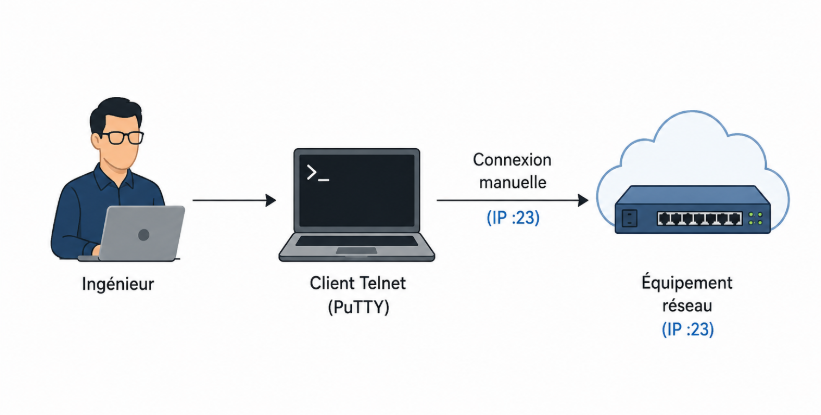
\includegraphics[width=0.88\textwidth]{images/systeme_existant}
  \caption{Schéma du processus de tests Telnet existant}
  \label{fig:systeme_existant}
\end{figure}

\subsection{Analyse critique de l'infrastructure actuelle}

\begin{table}[H]
  \centering
  \caption{Analyse critique du système de tests existant}
  \label{tab:analyse_critique}
  \begin{tabularx}{\textwidth}{|L{3cm}|L{4.5cm}|X|}
    \hline
    \textbf{Aspect} & \textbf{État actuel} & \textbf{Impact métier} \\
    \hline
    Connexion Telnet &
      Ouverture manuelle via PuTTY ou terminal &
      Risque élevé d'erreurs de saisie~; temps de connexion non optimisé \\
    \hline
    Supervision &
      Inexistante~; contrôle visuel uniquement &
      Aucune détection proactive des anomalies~; pannes non tracées \\
    \hline
    Scalabilité &
      Un seul test à la fois, un seul slot &
      Allongement des cycles de validation~; blocage des livraisons \\
    \hline
    Pipeline CI/CD &
      Absent~; déploiement manuel &
      Délais de mise en production importants~; risque de régression \\
    \hline
    Qualité et standardisation &
      Procédures non formalisées~; dépendance aux individus &
      Résultats non reproductibles~; difficulté d'audit \\
    \hline
    Reporting &
      Fichiers Excel manuels &
      Aucune centralisation~; données inutilisables pour l'analyse \\
    \hline
  \end{tabularx}
\end{table}

\noindent\textbf{Analyse des causes racines~:}
\begin{itemize}
  \item \textbf{Aucun outil dédié~:} il n'existait pas de plateforme
        conçue spécifiquement pour gérer des connexions Telnet multi-slots~;
  \item \textbf{Processus non industrialisé~:} aucune intégration dans
        une chaîne CI/CD~;
  \item \textbf{Données dispersées~:} configuration, commandes et résultats
        n'avaient pas de référentiel commun~;
  \item \textbf{Gestion des utilisateurs absente~:} ni contrôle d'accès,
        ni traçabilité des actions.
\end{itemize}

\subsection{Solution proposée}

La solution \textbf{Telnet Test Manager} couvre l'ensemble de ces
lacunes à travers trois composants principaux~:

\begin{enumerate}
  \item \textbf{Application web fullstack}
    \begin{itemize}
      \item Interface React~18/TypeScript pour la configuration et
            l'exécution des tests~;
      \item Backend Node.js/Express.js structuré selon la Clean
            Architecture~;
      \item Base de données MongoDB pour la persistance.
    \end{itemize}

  \item \textbf{Moteur de tests Telnet automatisé}
    \begin{itemize}
      \item Exécution isolée dans des Worker Threads Node.js~;
      \item Trois modes d'exécution~: commande unitaire, séquence
            d'étapes, supervision continue~;
      \item Tests multi-slots en parallèle~;
      \item Diffusion des résultats en temps réel via WebSocket.
    \end{itemize}

  \item \textbf{Infrastructure DevOps}
    \begin{itemize}
      \item Conteneurisation Docker avec build multi-stage pour
            le frontend~;
      \item Orchestration Kubernetes via chart Helm v0.3.0~;
      \item Autoscaling horizontal (HPA~: 1 à 5 répliques, seuil
            CPU à 70\,\%)~;
      \item Pipeline GitHub Actions en 3 jobs~: CI backend, CI
            frontend, déploiement~;
      \item Supervision Prometheus/Grafana avec 10 panneaux de
            métriques.
    \end{itemize}
\end{enumerate}

% -----------------------------------------------------------------
\section{Contexte et objectifs du projet}

\subsection{Contexte et historique}

Le besoin est venu directement du département d'ingénierie des tests
de Sagemcom Ezzahra. Avec la multiplication des familles de produits
--- passerelles xDSL, VDSL2, fibre, décodeurs IPTV --- et l'augmentation
du nombre de slots à valider par équipement, le processus manuel est
devenu difficile à tenir. Une première tentative basée sur des scripts
Python avait été envisagée, puis abandonnée par manque de centralisation
et d'interface utilisateur. Le projet s'est alors orienté vers une
application web moderne, évolutive et intégrée dans l'écosystème DevOps
existant.

\subsection{Méthodologie de travail}

\subsubsection{Mise en \oe{}uvre de la méthodologie Agile Scrum}

Le projet s'appuie sur la méthodologie \textbf{Agile Scrum} pour piloter
cette initiative d'automatisation. Cette approche apporte la flexibilité
et la capacité de livraison itérative nécessaires pour un projet de cette
complexité technique.

\paragraph{Apports du cadre Scrum~:}
\begin{itemize}
  \item \textbf{Livraison itérative~:} chaque composant d'infrastructure
        (moteur Telnet, conteneurisation, orchestration, CI/CD) est livré
        de façon incrémentale~;
  \item \textbf{Validation continue~:} chaque couche d'automatisation est
        vérifiée avant de passer à la suivante~;
  \item \textbf{Visibilité claire~:} toutes les parties prenantes suivent
        l'avancement en temps réel~;
  \item \textbf{Gestion des risques~:} les problèmes techniques ---
        compatibilité Docker, configuration Kubernetes, intégration
        WebSocket --- sont détectés et traités tôt~;
  \item \textbf{Alignement métier~:} les exigences techniques restent en
        phase avec les objectifs du projet tout au long du développement.
\end{itemize}

\paragraph{Structure des sprints~:}
\begin{itemize}
  \item \textbf{Durée~:} 2 semaines, adaptées aux cycles de livraison
        d'infrastructure~;
  \item \textbf{Sprint Planning~:} priorisation du backlog technique et
        allocation des ressources~;
  \item \textbf{Daily Scrums~:} synchronisation quotidienne et
        identification des blocages~;
  \item \textbf{Sprint Reviews~:} démonstration des livrables et retours
        des encadrants~;
  \item \textbf{Rétrospectives~:} amélioration continue du processus à
        chaque itération.
\end{itemize}

\begin{figure}[H]
  \centering
  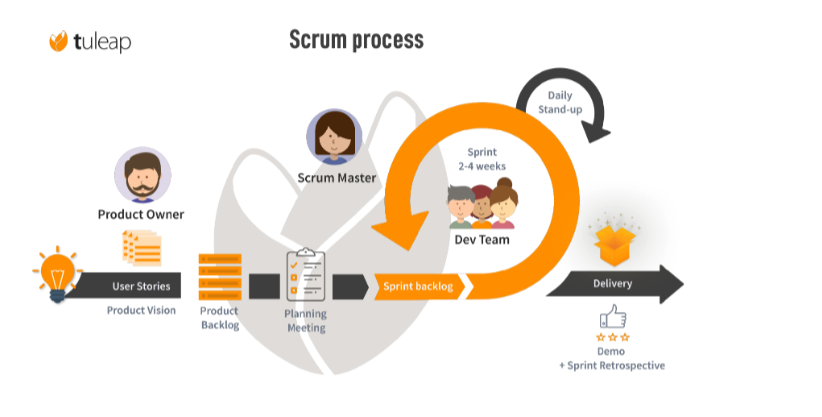
\includegraphics[width=0.88\textwidth]{images/scrum_process}
  \caption{Schéma du cadre Scrum appliqué au projet Telnet Test Manager}
  \label{fig:scrum_schema}
\end{figure}

Le schéma Scrum illustre le flux de travail complet adapté au projet.
Les sprints de deux semaines intègrent la gestion du backlog
d'infrastructure, la planification technique et les livrables. Les
Daily Scrums assurent la coordination entre les tâches DevOps,
l'implémentation de la sécurité et le développement des modules
applicatifs.

\subsubsection{Composition de l'équipe Scrum}

L'équipe est structurée pour répondre à la complexité technique et aux
exigences pluridisciplinaires du projet. Chaque rôle apporte une
expertise ciblée, dans un fonctionnement collaboratif orienté vers la
livraison d'une plateforme de tests prête pour la production.

\begin{table}[H]
  \centering
  \caption{Membres de l'équipe Scrum}
  \label{tab:equipe_scrum}
  \begin{tabularx}{\textwidth}{|L{2.8cm}|L{3.5cm}|X|}
    \hline
    \textbf{Rôle} & \textbf{Membre} & \textbf{Responsabilités principales} \\
    \hline
    Product Owner &
      Walid Ncir\newline\textit{(Encadrant Sagemcom)} &
      Définition des exigences métier, priorisation du backlog produit,
      validation des livrables et alignement avec les objectifs de
      l'équipe tests de Sagemcom Ezzahra \\
    \hline
    Scrum Master &
      Rim Tlili\newline\textit{(Encadrante académique)} &
      Facilitation du processus Scrum, levée des obstacles,
      application de la méthodologie agile et suivi de l'avancement
      académique du projet \\
    \hline
    Équipe de développement &
      Adem Hmercha\newline\textit{(Étudiant PFE)} &
      Conception de l'architecture système, développement fullstack
      (Node.js, React, MongoDB), implémentation du moteur Telnet et
      déploiement de l'infrastructure DevOps complète \\
    \hline
  \end{tabularx}
\end{table}

\section{Conclusion}

Ce chapitre a posé les bases nécessaires à la mise en place d'une
plateforme de tests Telnet automatisée et orientée DevOps au sein de
\textbf{Sagemcom Ezzahra}. L'analyse menée montre clairement où se
situent les manques~: automatisation absente, supervision inexistante,
traçabilité insuffisante --- autant de points qui ralentissent le
département et allongent les délais de livraison des firmwares validés.

La solution \textbf{Telnet Test Manager} répond à ces problèmes par
une approche DevOps structurée~: moteur d'exécution Telnet automatisé,
supervision temps réel via WebSocket, gestion centralisée des équipements
et pipeline CI/CD de bout en bout. Passer des opérations manuelles à une
plateforme automatisée, ce n'est pas juste une mise à jour technique ---
c'est une façon différente de travailler pour toute l'équipe d'ingénierie
des tests.

Avec une automatisation complète et une supervision en temps réel,
Sagemcom Ezzahra gagne en fiabilité, en traçabilité et en efficacité
sur la validation de ses équipements réseau embarqués. La méthodologie
\textbf{Agile Scrum} encadre cette transition en découpant la livraison
en sprints de deux semaines, chacun avec des critères de succès clairs,
ce qui permet de garder le contrôle sur la qualité, la sécurité et les
performances à chaque étape.

Cette analyse prépare les phases d'implémentation qui suivent, en fixant
des attentes précises sur les livrables, les délais et les métriques à
atteindre. L'architecture retenue --- Clean Architecture, WebSocket,
Docker, Kubernetes, GitHub Actions --- forme une base solide pour une
plateforme de tests durable et évolutive.

Au final, la réalisation de cette plateforme DevOps permettra à l'équipe
d'ingénierie de Sagemcom Ezzahra de valider ses firmwares embarqués plus
vite, avec une meilleure traçabilité et une productivité accrue ---
que ce soit avec la version actuelle de Telnet Test Manager ou ses
évolutions futures.


% =============================================================
%  Chapitre 2 — Analyse et spécification des besoins
% =============================================================
\chapter{Analyse et spécification des besoins}

\section{Introduction}

Ce chapitre détaille les besoins de l'application Telnet Test Manager.
On commence par identifier les acteurs du système, puis on passe aux
besoins fonctionnels et non fonctionnels. Le diagramme des cas
d'utilisation et les scénarios principaux complètent cette analyse.

% -----------------------------------------------------------------
\section{Identification des acteurs}
% -----------------------------------------------------------------

\subsection{Administrateur}

L'\textbf{Administrateur} a accès à toutes les fonctionnalités du
système. Il gère les comptes utilisateurs, configure les équipements,
consulte les journaux d'audit et suit les tests et rapports générés.

\subsection{Technicien}

Le \textbf{Technicien} est le principal utilisateur terrain. Son rôle
se limite à lancer des tests Telnet sur les équipements configurés,
consulter les résultats en temps réel et générer des rapports.

\subsection{Ingénieur}

L'\textbf{Ingénieur} s'occupe de la configuration des équipements et
de la bibliothèque de commandes Telnet. Il pilote les campagnes de
tests, analyse les résultats et produit des rapports. Il dispose de
tous les droits du Technicien, en plus des siens.

% -----------------------------------------------------------------
\section{Besoins fonctionnels}
% -----------------------------------------------------------------

\begin{table}[H]
  \centering
  \caption{Récapitulatif des besoins fonctionnels}
  \label{tab:besoins_fonctionnels}
  \begin{tabular}{|C{1cm}|L{3cm}|L{9.5cm}|}
    \hline
    \textbf{ID} & \textbf{Module} & \textbf{Description} \\
    \hline
    BF-01 & Authentification &
      Connexion JWT, RBAC (3 rôles), limitation de débit \\
    \hline
    BF-02 & Équipements &
      CRUD complet~: Poste / Produit / Slot / Référence \\
    \hline
    BF-03 & Commandes &
      Bibliothèque~: single, séquence, monitoring \\
    \hline
    BF-04 & Tests Telnet &
      Exécution, validation de réponse, arrêt à la demande \\
    \hline
    BF-05 & Multi-slots &
      Lancement parallèle via Worker Threads isolés \\
    \hline
    BF-06 & Temps réel &
      Diffusion des événements de test via WebSocket \\
    \hline
    BF-07 & Rapports &
      Compilation, filtrage, statistiques de campagne \\
    \hline
    BF-08 & Administration &
      Gestion utilisateurs, journal d'audit, analytiques \\
    \hline
    BF-09 & Monitoring &
      Métriques Prometheus, dashboards Grafana, alertes \\
    \hline
  \end{tabular}
\end{table}

% -----------------------------------------------------------------
\section{Besoins non fonctionnels}
% -----------------------------------------------------------------

\begin{table}[H]
  \centering
  \caption{Contraintes techniques et non fonctionnelles}
  \label{tab:besoins_non_fonctionnels}
  \begin{tabular}{|L{3cm}|L{4.5cm}|L{6cm}|}
    \hline
    \textbf{Catégorie} & \textbf{Exigence} & \textbf{Critère de mesure} \\
    \hline
    \multirow{2}{*}{\textbf{Performance}}
      & Temps de réponse API & 95\,\% des requêtes $<$ 2\,s \\
    \cline{2-3}
      & Parallélisme & 10 tests Telnet simultanés minimum \\
    \hline
    \multirow{3}{*}{\textbf{Sécurité}}
      & Authentification & JWT HS256, expiration configurable \\
    \cline{2-3}
      & Mots de passe & bcryptjs, coût~: 10 \\
    \cline{2-3}
      & En-têtes HTTP & Helmet.js~: CSP, HSTS, X-Frame \\
    \hline
    \textbf{Disponibilité}
      & Objectif de service & 99,9\,\% sur l'infrastructure locale \\
    \hline
    \multirow{2}{*}{\textbf{Scalabilité}}
      & Autoscaling & HPA~: 1--5 répliques, seuil CPU 70\,\% \\
    \cline{2-3}
      & Sans état & Backend stateless, session JWT \\
    \hline
    \textbf{Maintenabilité}
      & Architecture & Clean Architecture, principes SOLID \\
    \hline
    \textbf{Portabilité}
      & Conteneurisation & Images Docker identiques dev/production \\
    \hline
  \end{tabular}
\end{table}

% -----------------------------------------------------------------
\section{Diagramme des cas d'utilisation}
% -----------------------------------------------------------------

\begin{figure}[H]
  \centering
  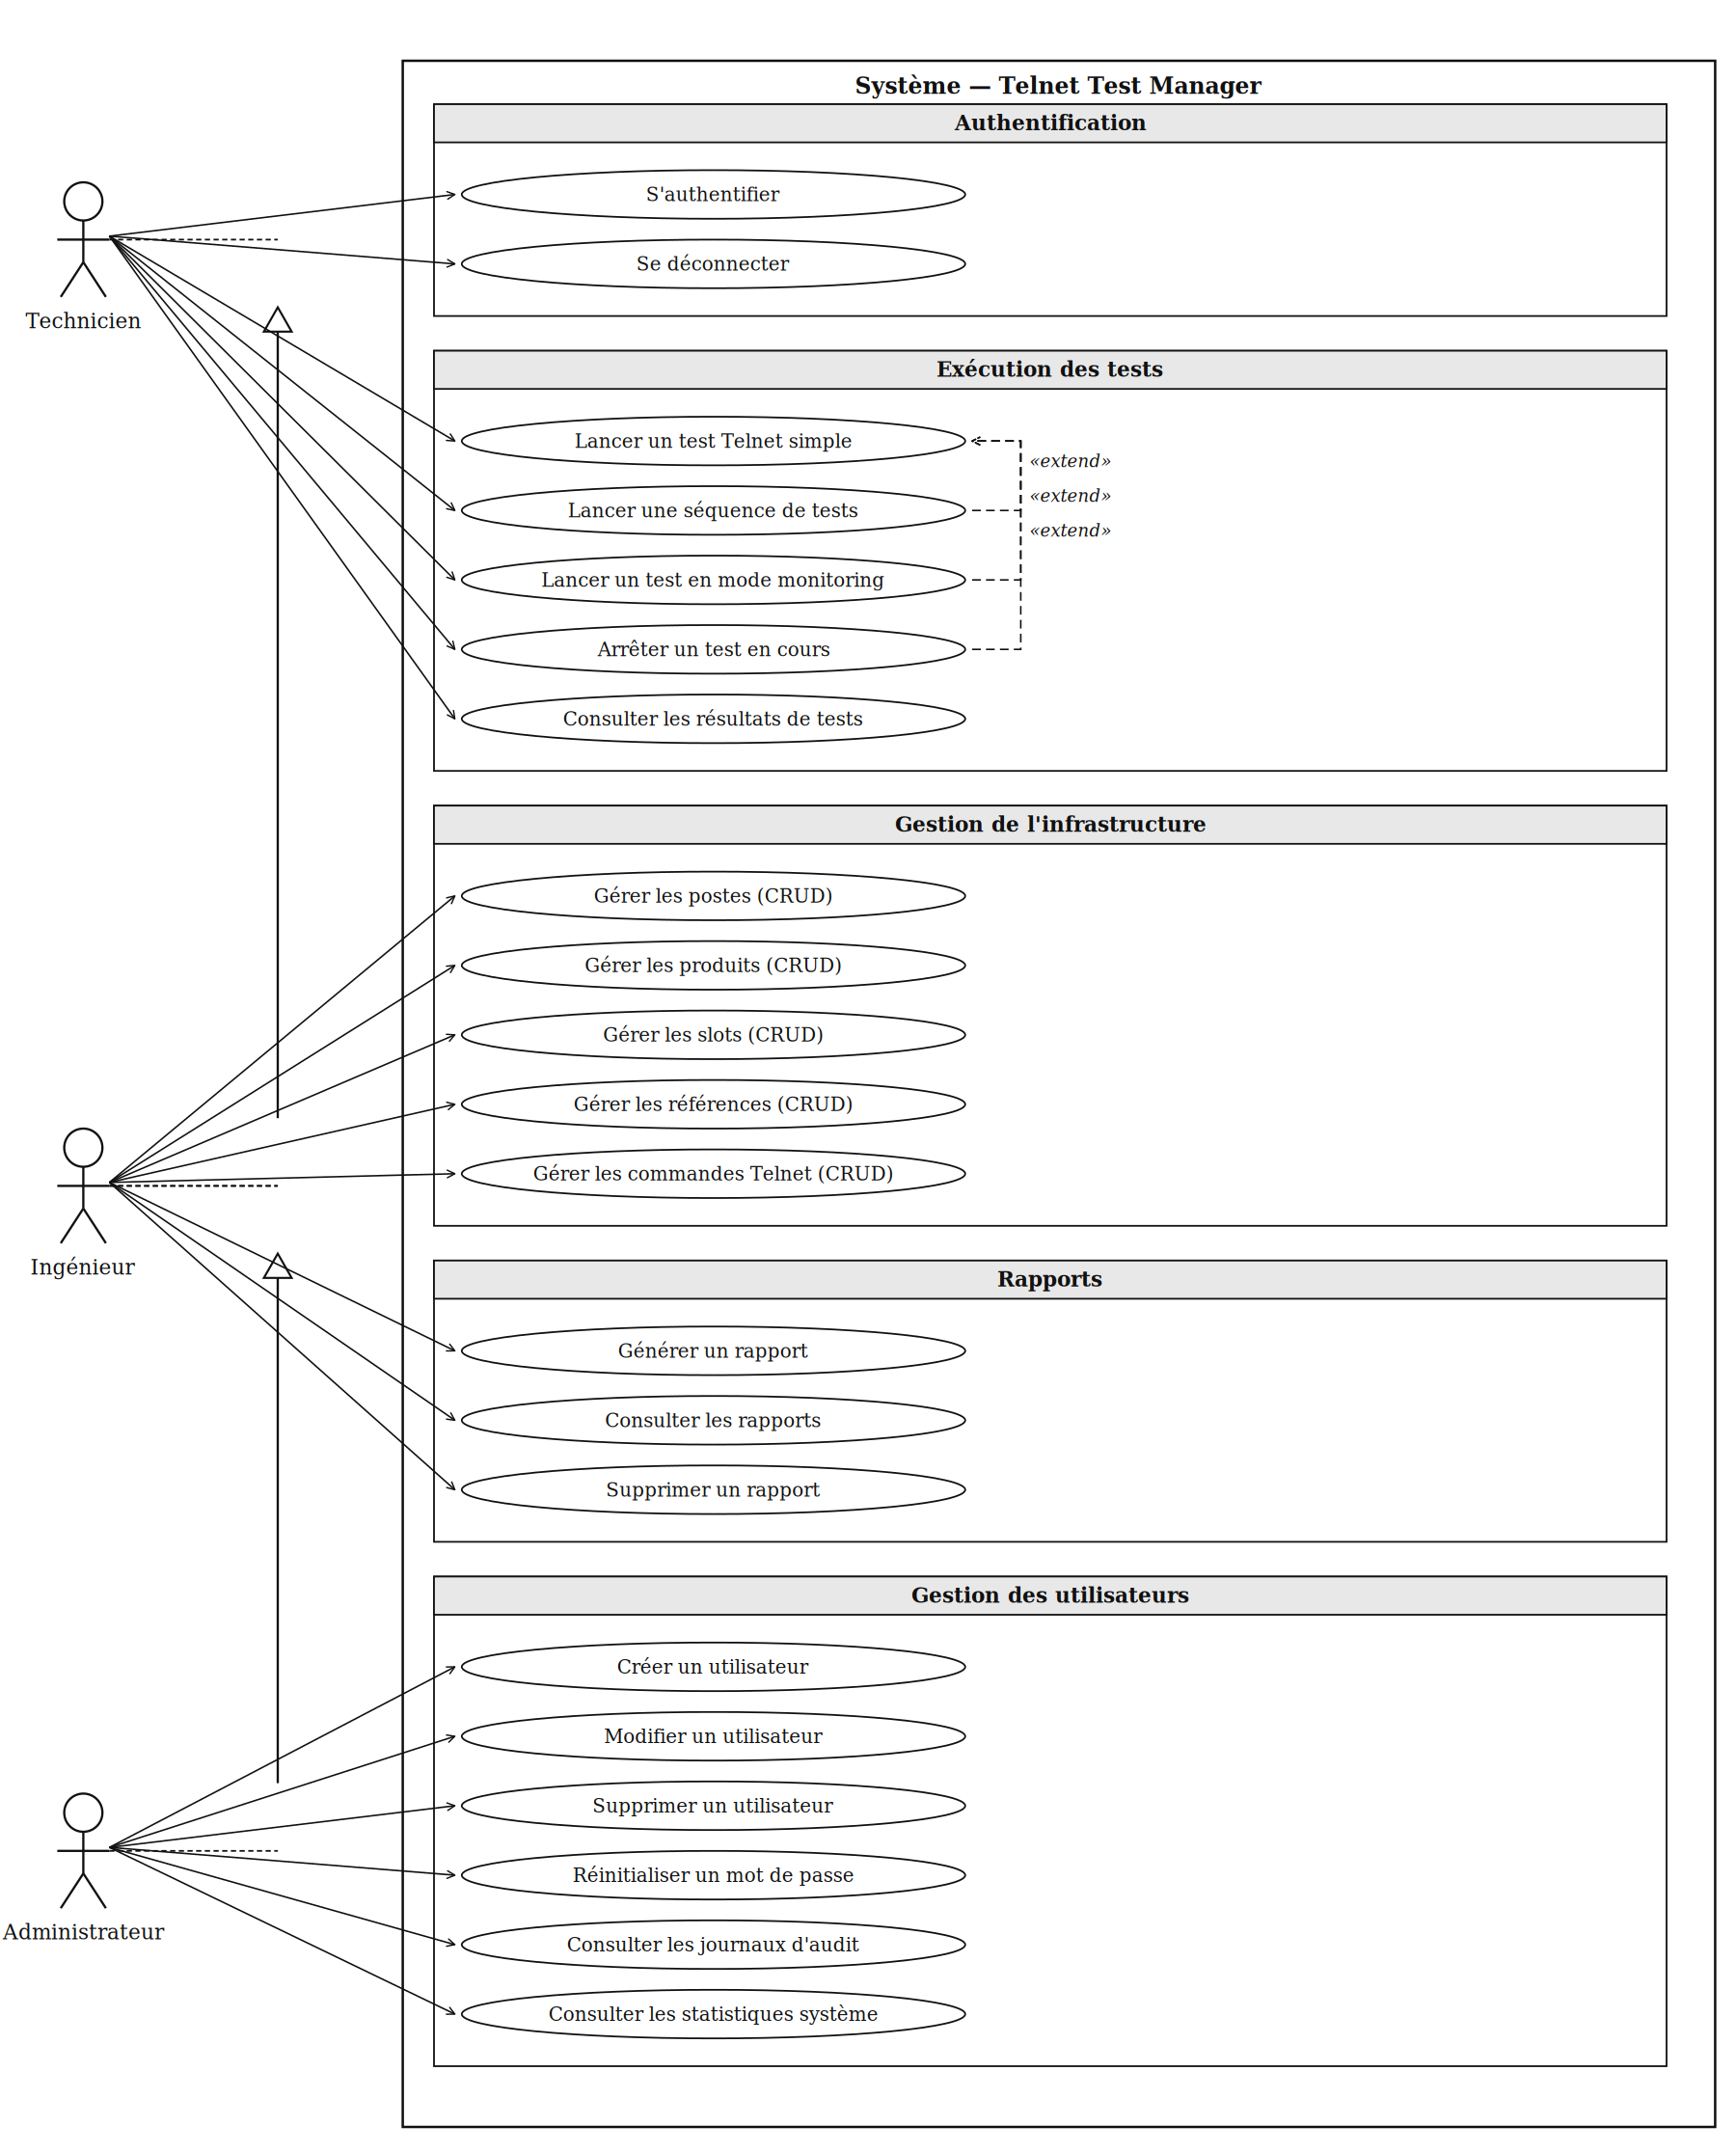
\includegraphics[width=\textwidth]{images/usecase_diagram}
  \caption{Diagramme des cas d'utilisation global --- Telnet Test Manager}
  \label{fig:usecase}
\end{figure}

% -----------------------------------------------------------------
\section{Description des cas d'utilisation principaux}
% -----------------------------------------------------------------

\begin{table}[H]
  \centering
  \caption{UC-01 --- S'authentifier}
  \label{tab:uc01}
  \begin{tabular}{|L{3.5cm}|L{10cm}|}
    \hline
    \textbf{Nom} & S'authentifier \\
    \hline
    \textbf{Acteurs} & Technicien, Ingénieur, Administrateur \\
    \hline
    \textbf{Préconditions} & L'utilisateur dispose d'un compte actif en base \\
    \hline
    \textbf{Postconditions} & Un jeton JWT est généré et stocké côté client \\
    \hline
    \textbf{Scénario nominal} &
      1.~L'acteur saisit son identifiant et son mot de passe \\
    & 2.~Le système vérifie les identifiants et le statut du compte \\
    & 3.~Le système génère un JWT signé HS256 \\
    & 4.~Le frontend stocke le token et redirige vers le Dashboard \\
    \hline
    \textbf{Alternatives} &
      A1.~Identifiants incorrects~: 401 «~Identifiants invalides~» \\
    & A2.~Compte inactif~: 401 «~Compte inactif~» \\
    & A3.~10 tentatives échouées~: 429, blocage 15\,min \\
    \hline
  \end{tabular}
\end{table}

\begin{table}[H]
  \centering
  \caption{UC-04 --- Lancer un test Telnet}
  \label{tab:uc04}
  \begin{tabular}{|L{3.5cm}|L{10cm}|}
    \hline
    \textbf{Nom} & Lancer un test Telnet \\
    \hline
    \textbf{Acteurs} & Technicien, Ingénieur \\
    \hline
    \textbf{Préconditions} & Utilisateur authentifié, slot configuré et équipement accessible \\
    \hline
    \textbf{Postconditions} & Résultat enregistré en base (SUCCESS, FAIL ou STOPPED) \\
    \hline
    \textbf{Scénario nominal} &
      1.~L'acteur sélectionne Poste, Produit, Slot et la commande \\
    & 2.~L'acteur clique «~Lancer le test~» \\
    & 3.~Le backend crée un résultat PENDING et spawne un Worker Thread \\
    & 4.~Le Worker établit la connexion TCP port 23 \\
    & 5.~Le Worker exécute la commande et valide la réponse \\
    & 6.~Chaque étape est diffusée en temps réel via WebSocket \\
    & 7.~Le résultat final est enregistré en MongoDB \\
    \hline
    \textbf{Alternatives} &
      A1.~Connexion TCP impossible~: timeout, statut FAIL \\
    & A2.~Réponse incorrecte~: sous-chaîne attendue absente, FAIL \\
    & A3.~L'acteur arrête le test~: \texttt{POST /stop-test}, statut STOPPED \\
    \hline
  \end{tabular}
\end{table}

\begin{table}[H]
  \centering
  \caption{UC-07 --- Générer un rapport}
  \label{tab:uc07}
  \begin{tabular}{|L{3.5cm}|L{10cm}|}
    \hline
    \textbf{Nom} & Générer un rapport \\
    \hline
    \textbf{Acteurs} & Technicien, Ingénieur, Administrateur \\
    \hline
    \textbf{Préconditions} & Des résultats de tests existent en base \\
    \hline
    \textbf{Postconditions} & Un rapport de synthèse est enregistré et affiché \\
    \hline
    \textbf{Scénario nominal} &
      1.~L'acteur applique des filtres (date, statut, slot) \\
    & 2.~Le frontend envoie POST /reports/generate \\
    & 3.~Le backend récupère les résultats filtrés depuis MongoDB \\
    & 4.~Le backend calcule taux de succès, durée moyenne, total \\
    & 5.~Le rapport est enregistré et retourné (201) \\
    & 6.~Le frontend affiche le rapport de synthèse \\
    \hline
    \textbf{Alternatives} &
      A1.~Aucun résultat ne correspond aux filtres~: 404 \\
    \hline
  \end{tabular}
\end{table}

\section{Conclusion}

Ce chapitre a permis de cadrer les besoins de Telnet Test Manager.
Les trois acteurs --- Administrateur, Ingénieur et Technicien ---
couvrent tous les rôles du système. Les neuf besoins fonctionnels
organisés par module couvrent le cycle complet des tests Telnet,
de la connexion à la génération des rapports. Les besoins non
fonctionnels fixent les contraintes de performance, sécurité,
scalabilité et disponibilité. Le chapitre suivant aborde la
conception et les choix architecturaux retenus.

% =============================================================
%  Chapitre 3 — Conception
% =============================================================
\chapter{Conception}

\section*{Introduction}
Ce chapitre présente les choix d'architecture et de conception retenus
pour Telnet Test Manager. On y trouve l'architecture générale, les
diagrammes de classes et de séquence des cas d'utilisation principaux,
et le modèle de données MongoDB.

% -----------------------------------------------------------------
\section{Architecture générale de l'application}
% -----------------------------------------------------------------

\subsection{Architecture globale du système}

\begin{figure}[H]
  \centering
  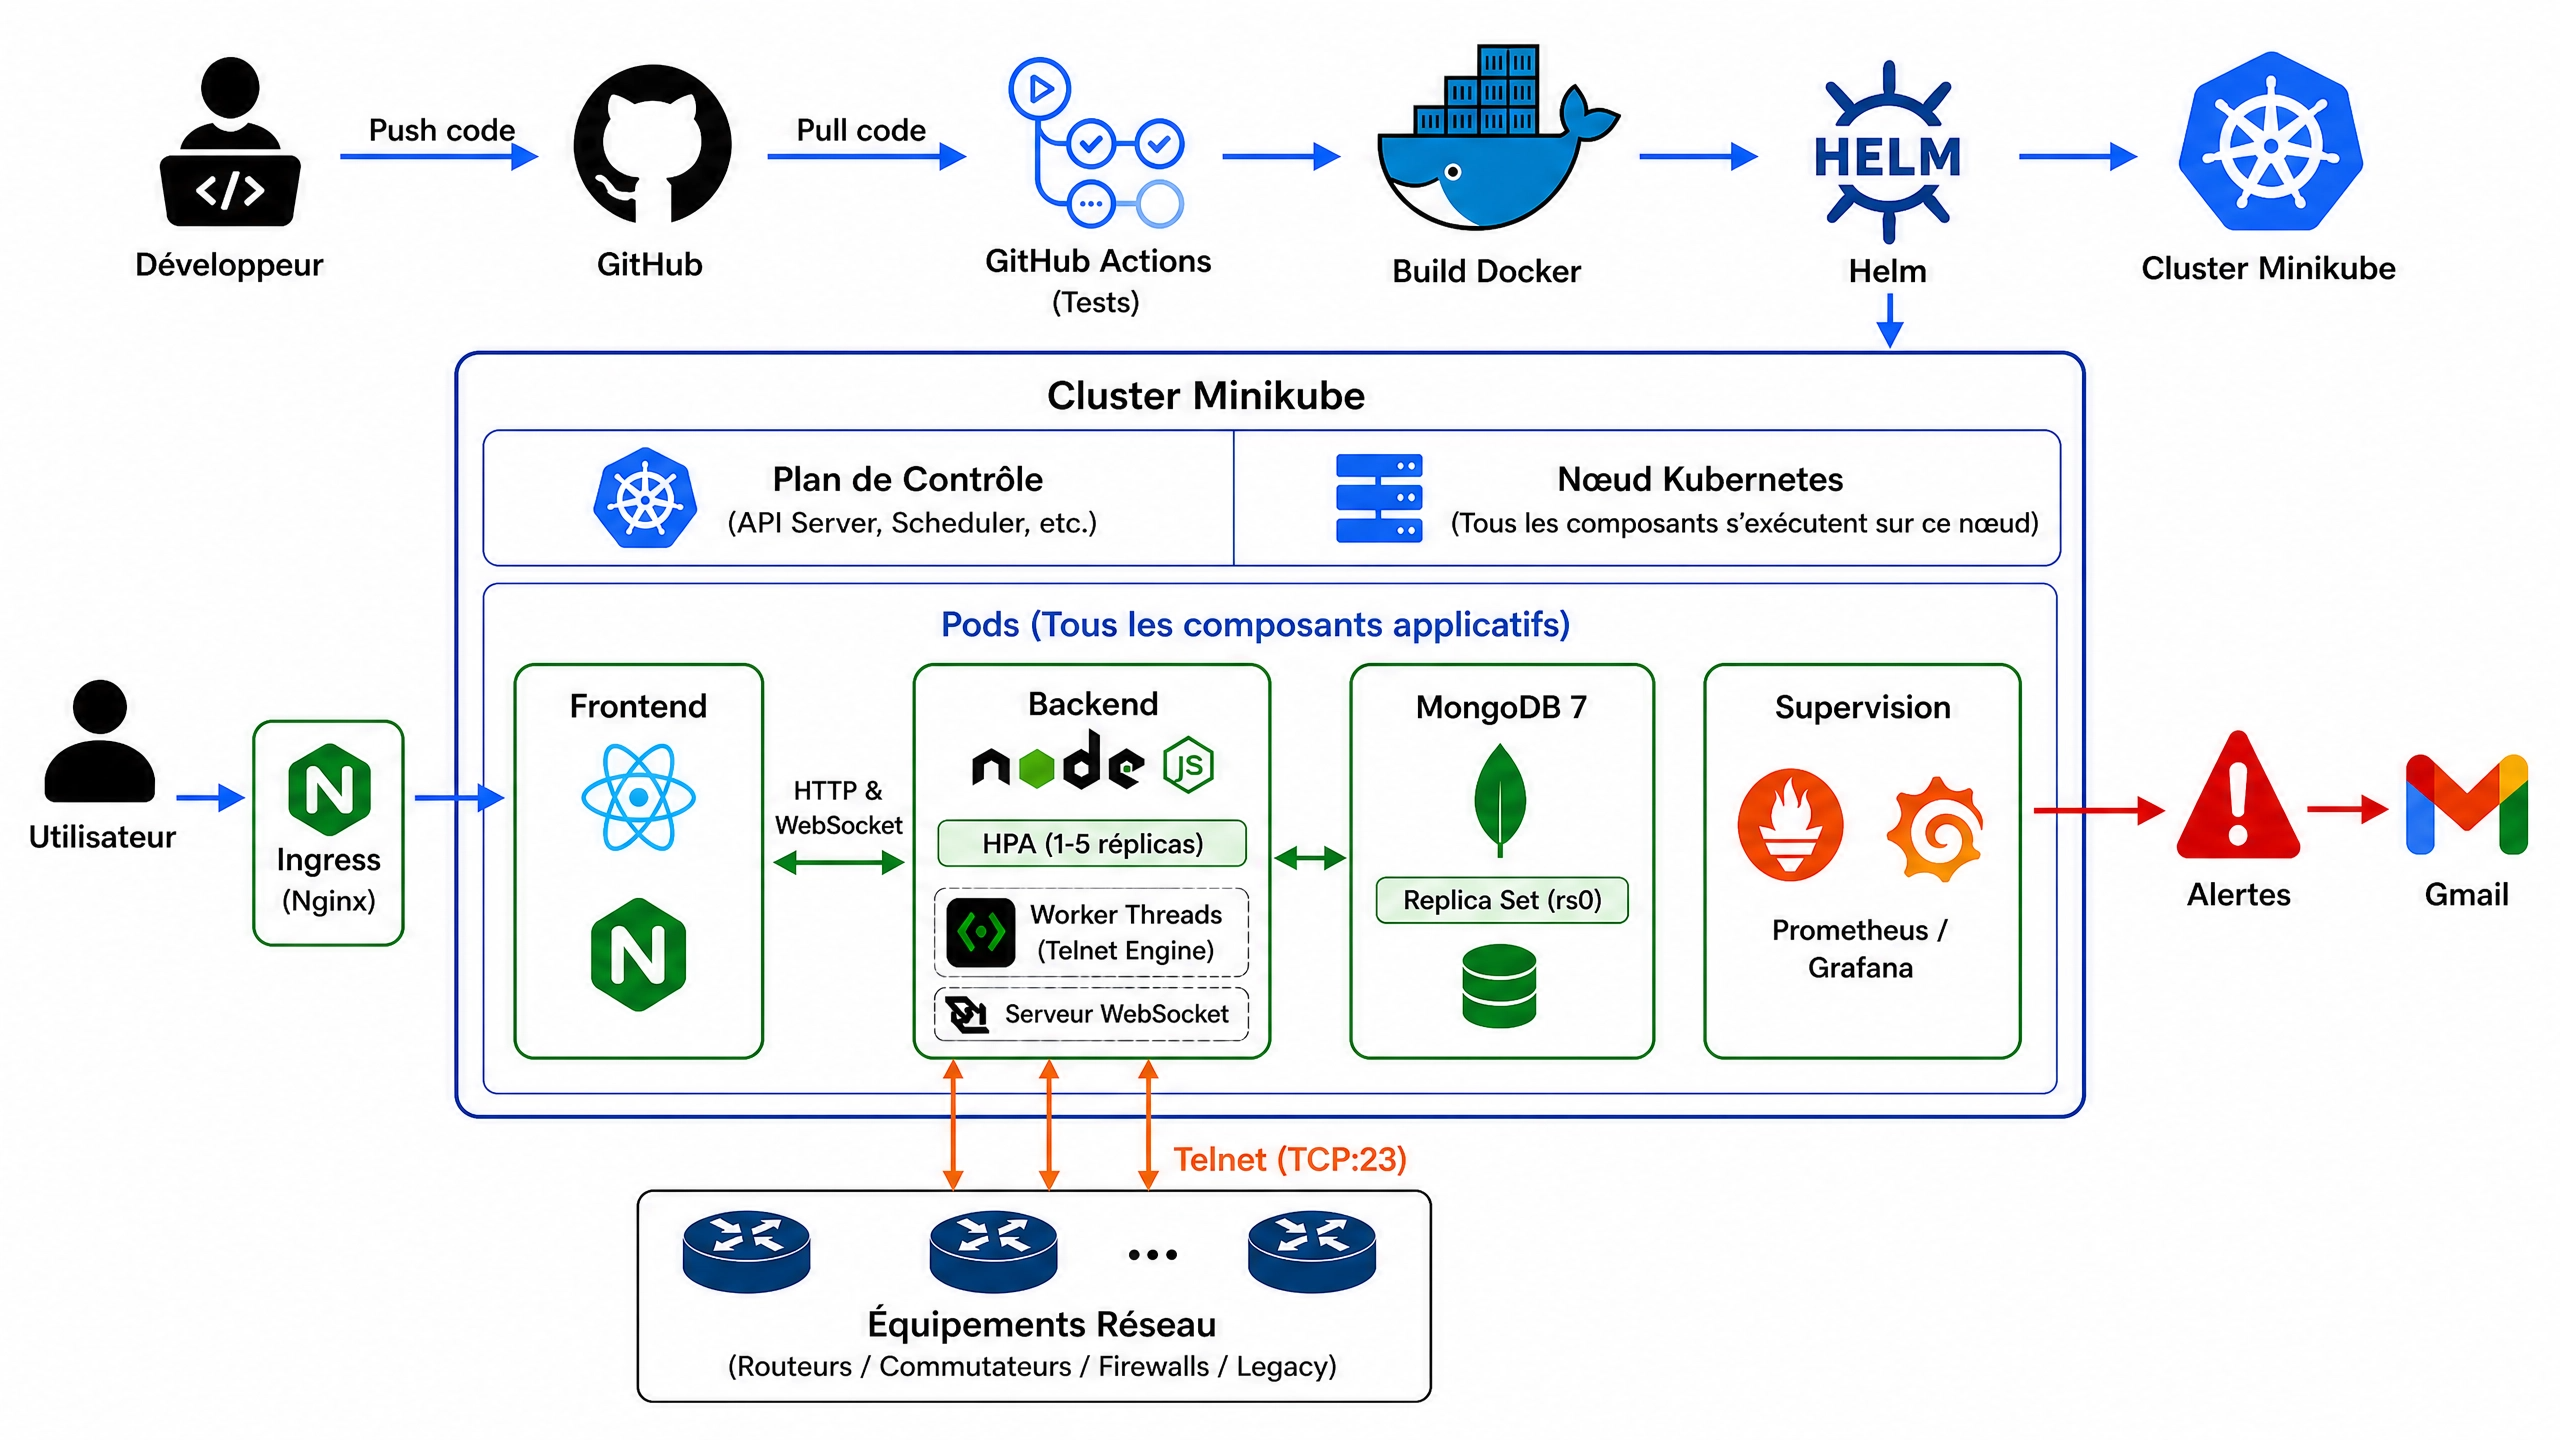
\includegraphics[width=\textwidth]{images/architecture_globale_finale}
  \caption{Architecture globale du système Telnet Test Manager}
  \label{fig:archi_globale}
\end{figure}

\subsection{Architecture N-tiers}

L'application est organisée selon une architecture \textbf{N-tiers} qui
sépare les responsabilités en couches distinctes~:

\begin{figure}[H]
  \centering
  \includegraphics[width=\textwidth]{"images/architecture N tiers"}
  \caption{Architecture N-tiers de l'application Telnet Test Manager}
  \label{fig:archi_ntiers}
\end{figure}

\subsection{Clean Architecture}

Le backend suit les principes de la \textbf{Clean Architecture}
\cite{martin2017clean}. L'idée centrale est simple~: les règles métier
ne dépendent d'aucun détail d'infrastructure. Les dépendances ne
peuvent pointer que \textit{vers l'intérieur}~:

\begin{figure}[H]
  \centering
  \includegraphics[width=0.75\textwidth]{"images/clean architecture"}
  \caption{Diagramme des couches de la Clean Architecture du backend}
  \label{fig:clean_archi}
\end{figure}

% -----------------------------------------------------------------
\section{Choix technologiques}
% -----------------------------------------------------------------

\subsubsection*{Développement Backend}

\subsection{Node.js / Express.js}

\textbf{Node.js} (v20 LTS) est un environnement d'exécution JavaScript
côté serveur basé sur le moteur V8. Son modèle non bloquant et le
support natif des Worker Threads le rendent bien adapté à un serveur
Telnet concurrent. \textbf{Express.js} (v4.18) structure l'application
en routes, middlewares et contrôleurs.

\begin{figure}[H]
  \centering
  
\includegraphics[width=0.28\textwidth]{images/nodejs}
  \caption{Logo Node.js / Express.js}
  \label{fig:logo_node}
\end{figure}

\subsection{MongoDB / Mongoose}

\textbf{MongoDB~7} est une base de données orientée documents (\gls{nosql}).
Son schéma flexible convient bien aux structures variables des résultats
de tests Telnet. \textbf{Mongoose~9} apporte la validation des schémas
et les middlewares d'accès aux données.

\begin{figure}[H]
  \centering
  
\includegraphics[width=0.28\textwidth]{images/mongodb}
  \caption{Logo MongoDB}
  \label{fig:logo_mongo}
\end{figure}

\subsubsection*{Développement Frontend}

\subsection{React 18 / TypeScript}

\textbf{React 18} avec \textbf{TypeScript} forme l'interface utilisateur.
Le typage statique réduit les erreurs et facilite la maintenance. Les
appels API passent tous par une instance \textbf{Axios} avec intercepteur
JWT. L'internationalisation (FR/EN/PT-BR) est assurée par \textbf{i18next}.

\begin{figure}[H]
  \centering
  \includegraphics[width=0.28\textwidth]{"images/react loogo"}
  \caption{Logo React 18 / TypeScript}
  \label{fig:logo_react}
\end{figure}

\subsubsection*{Outils DevOps}

\subsection{Docker}

\textbf{Docker} encapsule chaque service (backend, frontend, MongoDB)
dans des images autonomes et portables. Le frontend utilise un build
multi-stage qui ramène l'image de production à $\sim$25\,Mo.

\begin{figure}[H]
  \centering
  
\includegraphics[width=0.28\textwidth]{images/docker}
  \caption{Logo Docker}
  \label{fig:logo_docker}
\end{figure}

\subsection{Kubernetes}

\textbf{Kubernetes} (\gls{k8s}) orchestre les conteneurs en production.
Il gère le déploiement, la montée en charge (HPA) et la résilience
des services. L'environnement utilisé est \textbf{Minikube}, un cluster
local single-node.

\begin{figure}[H]
  \centering
  
\includegraphics[width=0.28\textwidth]{images/kubernetes}
  \caption{Logo Kubernetes}
  \label{fig:logo_k8s}
\end{figure}

\subsection{Helm}

\textbf{Helm} est le gestionnaire de paquets Kubernetes. Il permet de
paramétrer les manifestes YAML via des templates et un fichier
\texttt{values.yaml}, ce qui rend les déploiements reproductibles
et faciles à mettre à jour.

\begin{figure}[H]
  \centering
  
\includegraphics[width=0.22\textwidth]{images/helm}
  \caption{Logo Helm}
  \label{fig:logo_helm}
\end{figure}

\subsection{GitHub Actions}

\textbf{GitHub Actions} est la plateforme CI/CD intégrée à GitHub.
Les workflows sont définis en YAML et se déclenchent sur les événements
Git. Un \textbf{runner auto-hébergé} donne accès au cluster Minikube
local sans avoir à exposer l'infrastructure sur Internet.

\begin{figure}[H]
  \centering
  
\includegraphics[width=0.30\textwidth]{images/githubactions}
  \caption{Logo GitHub Actions}
  \label{fig:logo_ghactions}
\end{figure}

\subsection{Prometheus}

\textbf{Prometheus} collecte les métriques en interrogeant périodiquement
l'endpoint \texttt{/metrics} du backend. Quatre métriques personnalisées
sont définies~: requêtes HTTP, durées de réponse, tests Telnet lancés
et connexions WebSocket actives.

\begin{figure}[H]
  \centering
  \includegraphics[width=0.28\textwidth]{"images/promtheus logo"}
  \caption{Logo Prometheus}
  \label{fig:logo_prometheus}
\end{figure}

\subsection{Grafana}

\textbf{Grafana} visualise les métriques collectées par Prometheus.
Le tableau de bord du projet contient 12 panneaux (CPU, mémoire,
latences HTTP, répliques HPA, WebSocket) et envoie des alertes
e-mail automatiques en cas de dépassement de seuil.

\begin{figure}[H]
  \centering
  
\includegraphics[width=0.25\textwidth]{images/grafana}
  \caption{Logo Grafana}
  \label{fig:logo_grafana}
\end{figure}

% -----------------------------------------------------------------
\section{Diagramme de classes}
% -----------------------------------------------------------------

\begin{figure}[H]
  \centering
  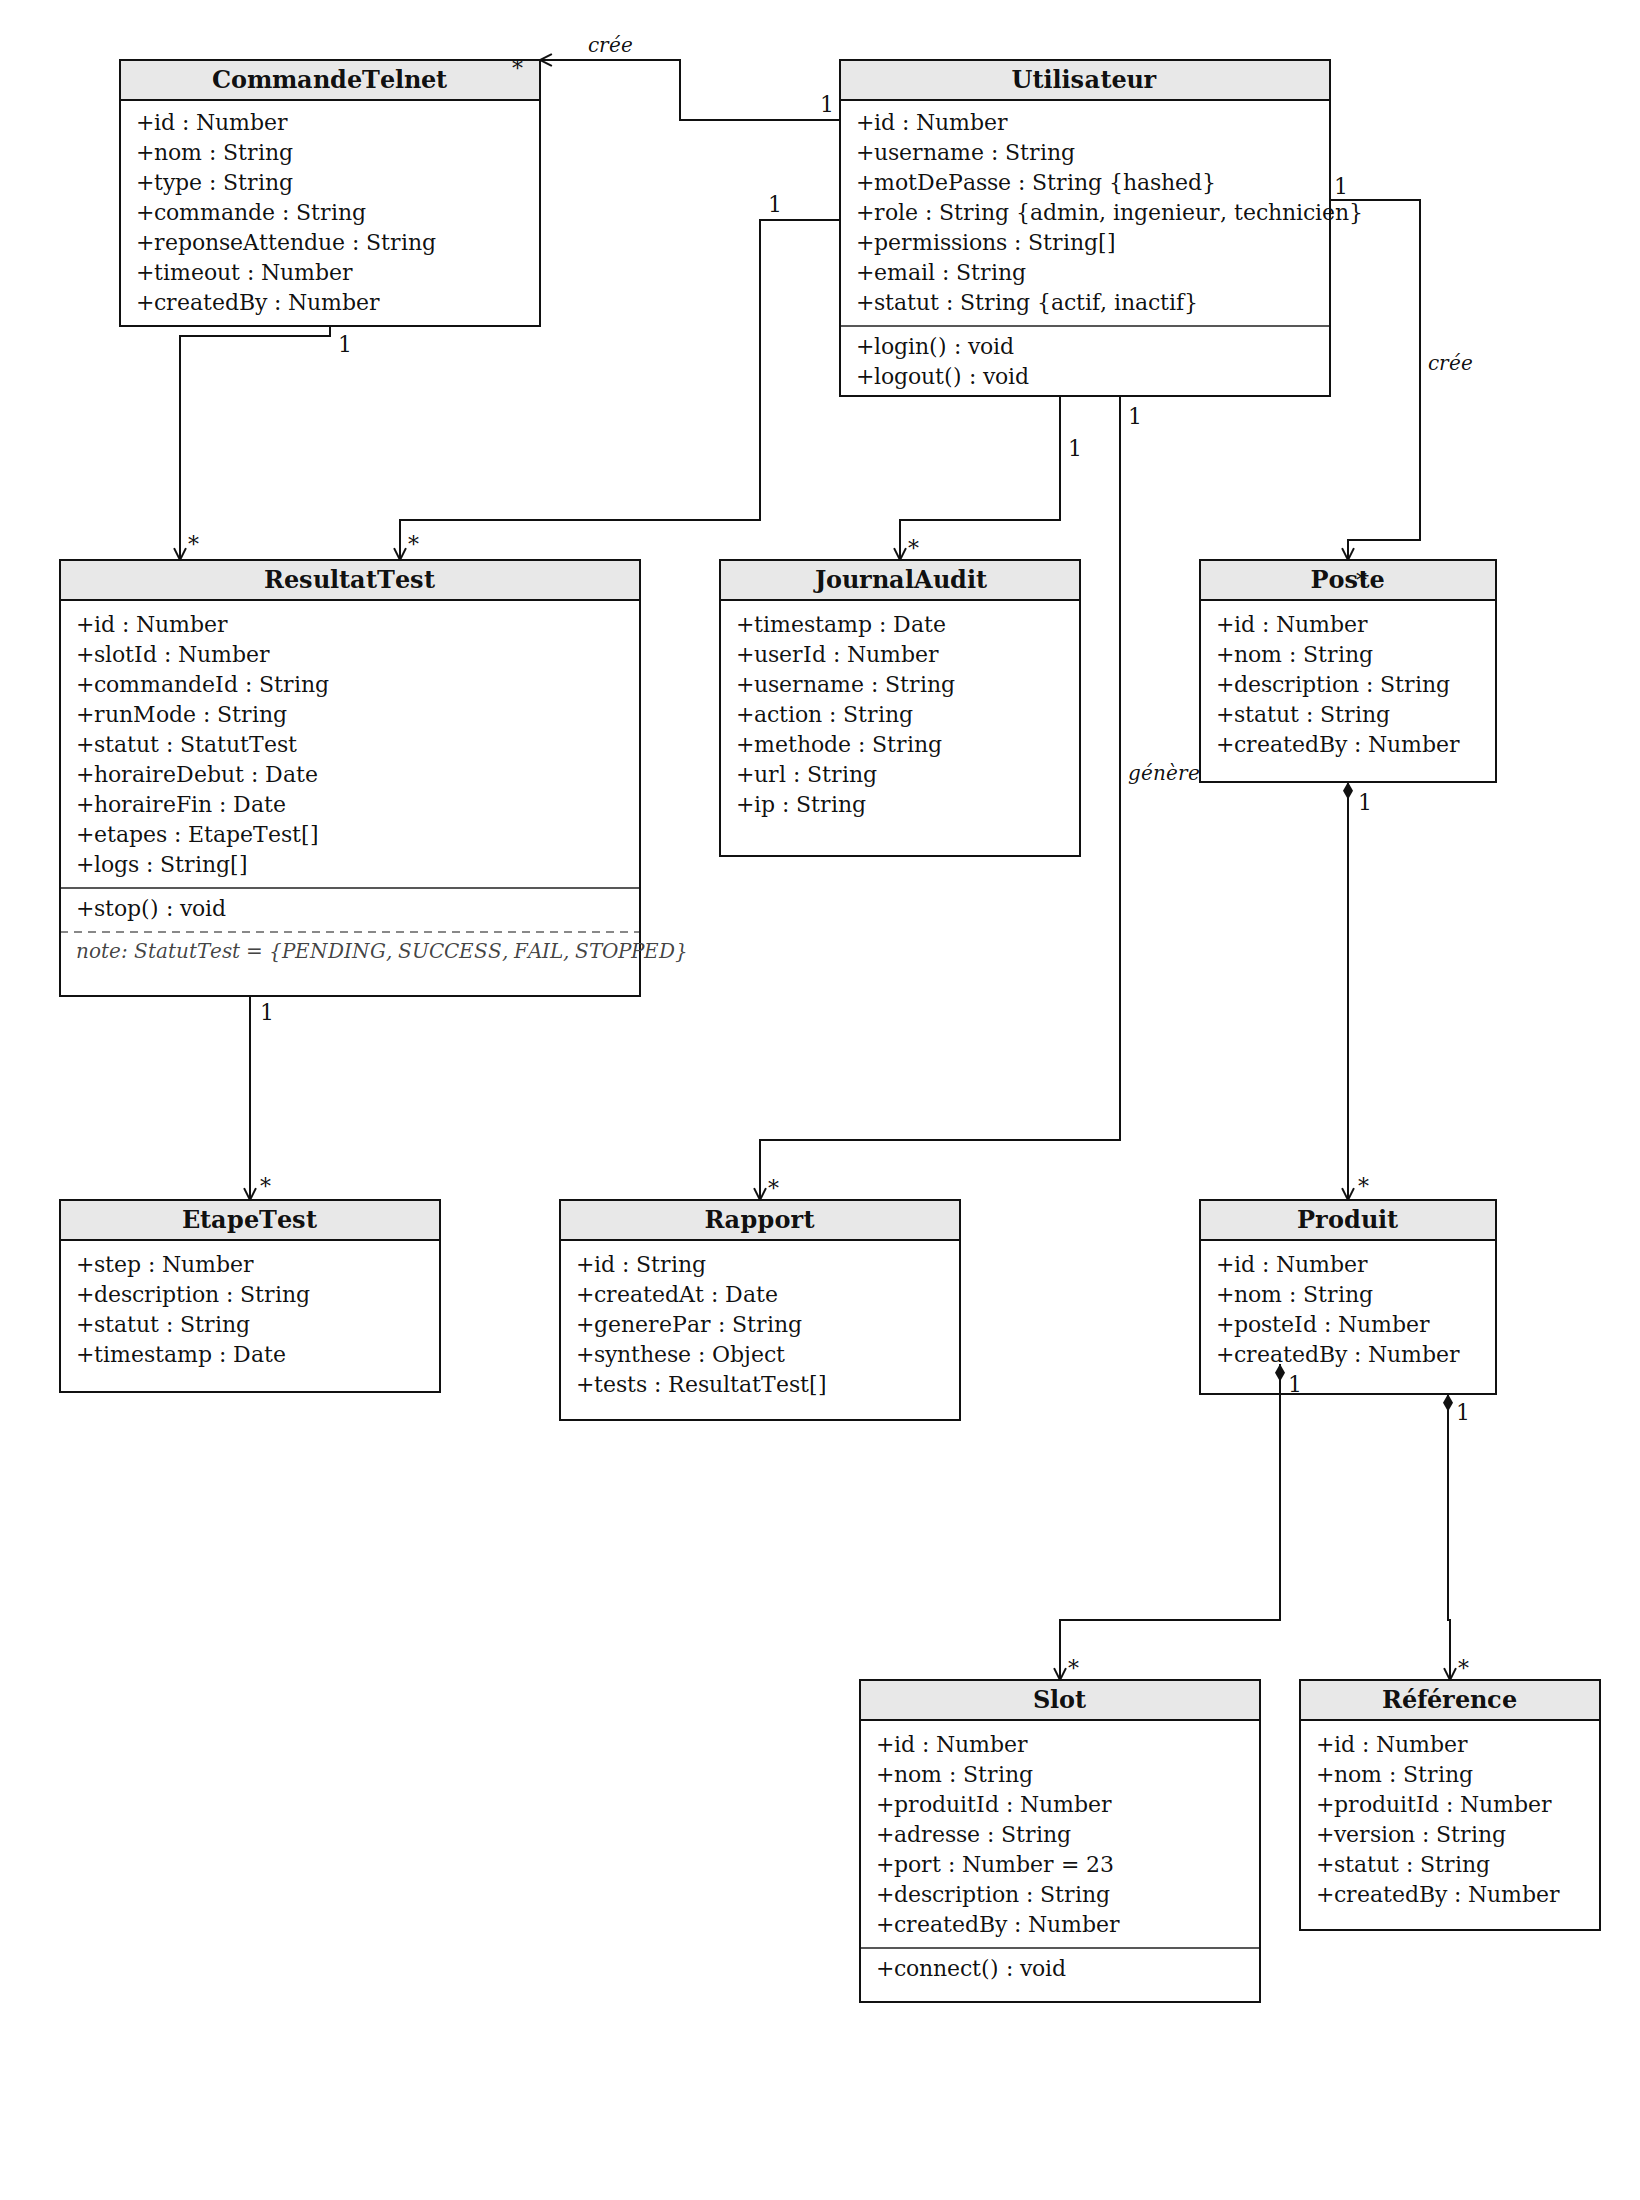
\includegraphics[width=\textwidth]{images/diagramclass}
  \caption{Diagramme de classes principal de Telnet Test Manager}
  \label{fig:class_diagram}
\end{figure}

% -----------------------------------------------------------------
\section{Diagrammes de séquence}
% -----------------------------------------------------------------

\subsection{Cas d'utilisation~: Authentification}

\begin{figure}[H]
  \centering
  \begin{tikzpicture}[
    life/.style={dashed,draw=gray!50},
    box/.style={draw=bleuPFE,fill=bleuPFE!8,minimum width=2.4cm,
                minimum height=0.6cm,align=center,font=\scriptsize},
    msg/.style={->,>=stealth,draw=bleuPFE,font=\scriptsize},
    ret/.style={->,>=stealth,draw=bleuPFE!50,dashed,font=\scriptsize},
    act/.style={draw=bleuPFE,fill=bleuPFE!20,minimum width=0.3cm,
                minimum height=1.2cm},
  ]

    % Participants
    \node[box] (user)  at (0,0)  {Utilisateur};
    \node[box] (front) at (3.5,0) {Frontend\\React};
    \node[box] (back)  at (7,0)  {Backend\\API};
    \node[box] (db)    at (10.5,0) {MongoDB};

    % Lifelines
    \draw[life] (0,-0.3) -- (0,-9);
    \draw[life] (3.5,-0.3) -- (3.5,-9);
    \draw[life] (7,-0.3) -- (7,-9);
    \draw[life] (10.5,-0.3) -- (10.5,-9);

    % Messages
    \draw[msg] (0,-1) -- (3.5,-1)
      node[midway,above,font=\scriptsize] {Saisie identifiants};
    \draw[msg] (3.5,-1.8) -- (7,-1.8)
      node[midway,above,font=\scriptsize] {\texttt{POST /login}};
    \draw[msg] (7,-2.6) -- (10.5,-2.6)
      node[midway,above,font=\scriptsize] {\texttt{findUser(username)}};
    \draw[ret] (10.5,-3.2) -- (7,-3.2)
      node[midway,above,font=\scriptsize] {User \{hash\}};
    \draw[msg] (7,-4) -- (7,-4)
      node[right,font=\scriptsize] {bcrypt.compare(mdp, hash)};
    \node[font=\scriptsize,color=gray,right] at (7.2,-4.7)
      {[succès] Génération JWT};
    \draw[ret] (7,-5.4) -- (3.5,-5.4)
      node[midway,above,font=\scriptsize]
      {200~: \{token, user\}};
    \draw[msg] (3.5,-6.2) -- (3.5,-6.2)
      node[right,font=\scriptsize]
      {Stockage token (sessionStorage)};
    \draw[ret] (3.5,-7) -- (0,-7)
      node[midway,above,font=\scriptsize] {Redirection Dashboard};

    % Fragment alt
    \draw[draw=bleuPFE!30,dashed] (1.5,-3) rectangle (9,-5);
    \node[font=\scriptsize\bfseries\color{bleuPFE!60}] at (2,-3.1)
      {[alt] Échec};
    \draw[ret] (7,-4.9) -- (3.5,-4.9)
      node[midway,above,font=\scriptsize] {401~: Identifiants invalides};

  \end{tikzpicture}
  \caption{Diagramme de séquence~: Authentification JWT}
  \label{fig:seq_auth}
\end{figure}

\subsection{Cas d'utilisation~: Exécution d'un test Telnet}

\begin{figure}[H]
  \centering
  \begin{tikzpicture}[
    life/.style={dashed,draw=gray!50},
    box/.style={draw=bleuPFE,fill=bleuPFE!8,minimum width=2.1cm,
                minimum height=0.6cm,align=center,font=\tiny},
    msg/.style={->,>=stealth,draw=bleuPFE,font=\tiny},
    ret/.style={->,>=stealth,draw=bleuPFE!50,dashed,font=\tiny},
  ]

    % Participants
    \node[box] (user)   at (0,0)    {Utilisateur};
    \node[box] (front)  at (2.5,0)  {Frontend};
    \node[box] (back)   at (5.5,0)  {Backend API};
    \node[box] (worker) at (8.5,0)  {Worker Thread};
    \node[box] (db)     at (11.2,0) {MongoDB};
    \node[box] (equip)  at (13.8,0) {Équipement\\TCP:23};

    % Lifelines
    \foreach \x in {0,2.5,5.5,8.5,11.2,13.8}
      \draw[life] (\x,-0.3) -- (\x,-13);

    % Messages
    \draw[msg] (0,-1)    -- (2.5,-1)
      node[midway,above] {Clic «Lancer le test»};
    \draw[msg] (2.5,-1.8) -- (5.5,-1.8)
      node[midway,above] {\texttt{POST /run-test}};
    \draw[msg] (5.5,-2.6) -- (5.5,-2.6)
      node[right] {Vérif. JWT \& permissions};
    \draw[msg] (5.5,-3.4) -- (11.2,-3.4)
      node[midway,above] {findSlot(slotId)};
    \draw[ret] (11.2,-4) -- (5.5,-4)
      node[midway,above] {Slot \{IP, port\}};
    \draw[msg] (5.5,-4.8) -- (11.2,-4.8)
      node[midway,above] {createTestResult (PENDING)};
    \draw[msg] (5.5,-5.6) -- (8.5,-5.6)
      node[midway,above] {spawnWorker(testId, slot, cmd)};
    \draw[ret] (5.5,-6.2) -- (2.5,-6.2)
      node[midway,above] {200~: \{testId\}};
    \draw[ret] (2.5,-6.9) -- (0,-6.9)
      node[midway,above] {Affichage «En cours...»};

    % Worker
    \draw[msg] (8.5,-7.7) -- (13.8,-7.7)
      node[midway,above] {Connexion TCP port 23};
    \draw[msg] (8.5,-8.4) -- (13.8,-8.4)
      node[midway,above] {Authentification (login/mdp)};
    \draw[msg] (8.5,-9.1) -- (13.8,-9.1)
      node[midway,above] {Envoi commande Linux};
    \draw[ret] (13.8,-9.8) -- (8.5,-9.8)
      node[midway,above] {Réponse Telnet};
    \draw[msg] (8.5,-10.5) -- (8.5,-10.5)
      node[right] {Comparaison expectedResponse};
    \draw[msg] (8.5,-11.2) -- (5.5,-11.2)
      node[midway,above] {WS~: \{step, status\}};
    \draw[msg] (5.5,-11.2) -- (2.5,-11.2);
    \draw[ret] (2.5,-11.2) -- (0,-11.2)
      node[midway,above] {Mise à jour UI (temps réel)};
    \draw[msg] (8.5,-12) -- (11.2,-12)
      node[midway,above] {updateTestResult (SUCCESS)};

  \end{tikzpicture}
  \caption{Diagramme de séquence~: Exécution d'un test Telnet}
  \label{fig:seq_telnet}
\end{figure}

\subsection{Cas d'utilisation~: Gestion CRUD des équipements}

\begin{figure}[H]
  \centering
  \begin{tikzpicture}[
    life/.style={dashed,draw=gray!50},
    box/.style={draw=bleuPFE,fill=bleuPFE!8,minimum width=2.4cm,
                minimum height=0.6cm,align=center,font=\scriptsize},
    msg/.style={->,>=stealth,draw=bleuPFE,font=\scriptsize},
    ret/.style={->,>=stealth,draw=bleuPFE!50,dashed,font=\scriptsize},
  ]
    \node[box] (ing)   at (0,0)    {Ingénieur};
    \node[box] (front) at (3.5,0)  {Frontend\\React};
    \node[box] (back)  at (7,0)    {Backend\\API};
    \node[box] (db)    at (10.5,0) {MongoDB};

    \draw[life] (0,-0.3)    -- (0,-9);
    \draw[life] (3.5,-0.3)  -- (3.5,-9);
    \draw[life] (7,-0.3)    -- (7,-9);
    \draw[life] (10.5,-0.3) -- (10.5,-9);

    \draw[msg] (0,-1)    -- (3.5,-1)
      node[midway,above] {Clic «Ajouter un poste»};
    \draw[ret] (3.5,-1.8) -- (0,-1.8)
      node[midway,above] {Affichage formulaire modal};
    \draw[msg] (0,-2.6)  -- (3.5,-2.6)
      node[midway,above] {Saisie nom + description};
    \draw[msg] (3.5,-3.4) -- (7,-3.4)
      node[midway,above] {\texttt{POST /postes \{nom, desc\}}};
    \draw[msg] (7,-4.2)  -- (7,-4.2)
      node[right] {Vérif. JWT + rôle Ingénieur};
    \draw[msg] (7,-5)    -- (10.5,-5)
      node[midway,above] {\texttt{PosteRepo.create(poste)}};
    \draw[ret] (10.5,-5.7) -- (7,-5.7)
      node[midway,above] {\{id: N, nom, createdAt\}};
    \draw[ret] (7,-6.5)  -- (3.5,-6.5)
      node[midway,above] {201~: poste créé};
    \draw[msg] (3.5,-7.3) -- (3.5,-7.3)
      node[right] {Actualise la liste};
    \draw[ret] (3.5,-8.1) -- (0,-8.1)
      node[midway,above] {Notification «Succès»};

    \draw[draw=bleuPFE!25,dashed] (1.5,-6) rectangle (5,-8.7);
    \node[font=\scriptsize\bfseries\color{bleuPFE!60}] at (2.1,-6.1)
      {[alt] PUT/DELETE};
  \end{tikzpicture}
  \caption{Diagramme de séquence~: Création d'un équipement (CRUD)}
  \label{fig:seq_crud}
\end{figure}

\subsection{Cas d'utilisation~: Tests multi-slots en parallèle}

\begin{figure}[H]
  \centering
  \begin{tikzpicture}[
    life/.style={dashed,draw=gray!50},
    box/.style={draw=bleuPFE,fill=bleuPFE!8,minimum width=1.8cm,
                minimum height=0.6cm,align=center,font=\tiny},
    msg/.style={->,>=stealth,draw=bleuPFE,font=\tiny},
    ret/.style={->,>=stealth,draw=bleuPFE!50,dashed,font=\tiny},
  ]
    \node[box] (ing)   at (0,0)    {Ingénieur};
    \node[box] (front) at (2.5,0)  {Frontend};
    \node[box] (back)  at (5.5,0)  {Backend};
    \node[box] (w1)    at (8.5,0)  {Worker 1\\(Slot A)};
    \node[box] (w2)    at (11,0)   {Worker 2\\(Slot B)};
    \node[box] (db)    at (13.5,0) {MongoDB};

    \foreach \x in {0,2.5,5.5,8.5,11,13.5}
      \draw[life] (\x,-0.3) -- (\x,-13.5);

    \draw[msg] (0,-1) -- (2.5,-1)
      node[midway,above] {Sélection 2 slots + commande};
    \draw[msg] (2.5,-1.8) -- (5.5,-1.8)
      node[midway,above] {\texttt{POST /run-test \{slotIds:[A,B]\}}};
    \draw[msg] (5.5,-2.6) -- (13.5,-2.6)
      node[midway,above] {createTestResults ×2 (PENDING)};
    \draw[msg] (5.5,-3.4) -- (8.5,-3.4)
      node[midway,above] {spawnWorker(id1, slotA)};
    \draw[msg] (5.5,-4)   -- (11,-4)
      node[midway,above] {spawnWorker(id2, slotB)};
    \draw[ret] (5.5,-4.8) -- (2.5,-4.8)
      node[midway,above] {200~: \{testIds:[1,2]\}};
    \draw[ret] (2.5,-5.4) -- (0,-5.4)
      node[midway,above] {Affiche «En cours (×2)»};

    \draw[draw=bleuPFE!25,dashed] (6,-6.2) rectangle (14.5,-12.5);
    \node[font=\tiny\bfseries\color{bleuPFE!60}] at (7.2,-6.3)
      {par (parallèle)};

    \draw[msg] (8.5,-6.8)  -- (8.5,-6.8)  node[right] {TCP SlotA:23 + auth + cmd};
    \draw[msg] (8.5,-7.5)  -- (5.5,-7.5)  node[midway,above] {WS~: step SUCCESS};
    \draw[msg] (8.5,-8.2)  -- (13.5,-8.2) node[midway,above] {updateResult (SUCCESS)};

    \draw[msg] (11,-9.2)   -- (11,-9.2)   node[right] {TCP SlotB:23 + auth + cmd};
    \draw[msg] (11,-9.9)   -- (5.5,-9.9)  node[midway,above] {WS~: step FAIL};
    \draw[msg] (11,-10.6)  -- (13.5,-10.6)node[midway,above] {updateResult (FAIL)};

    \draw[msg] (5.5,-11.5) -- (2.5,-11.5)
      node[midway,above] {WS broadcast résultats finals};
    \draw[ret] (2.5,-12.3) -- (0,-12.3)
      node[midway,above] {UI~: SUCCESS/FAIL par slot};

  \end{tikzpicture}
  \caption{Diagramme de séquence~: Tests multi-slots en parallèle}
  \label{fig:seq_multislot}
\end{figure}

\subsection{Cas d'utilisation~: Génération de rapport}

\begin{figure}[H]
  \centering
  \begin{tikzpicture}[
    life/.style={dashed,draw=gray!50},
    box/.style={draw=bleuPFE,fill=bleuPFE!8,minimum width=2.4cm,
                minimum height=0.6cm,align=center,font=\scriptsize},
    msg/.style={->,>=stealth,draw=bleuPFE,font=\scriptsize},
    ret/.style={->,>=stealth,draw=bleuPFE!50,dashed,font=\scriptsize},
  ]
    \node[box] (ing)   at (0,0)    {Ingénieur};
    \node[box] (front) at (3.5,0)  {Frontend\\React};
    \node[box] (back)  at (7,0)    {Backend\\API};
    \node[box] (db)    at (10.5,0) {MongoDB};

    \draw[life] (0,-0.3)    -- (0,-9.5);
    \draw[life] (3.5,-0.3)  -- (3.5,-9.5);
    \draw[life] (7,-0.3)    -- (7,-9.5);
    \draw[life] (10.5,-0.3) -- (10.5,-9.5);

    \draw[msg] (0,-1)    -- (3.5,-1)
      node[midway,above] {Filtre par date, statut, slot};
    \draw[msg] (3.5,-1.8) -- (7,-1.8)
      node[midway,above] {\texttt{POST /reports/generate \{filters\}}};
    \draw[msg] (7,-2.6)  -- (10.5,-2.6)
      node[midway,above] {findTestResults(filters)};
    \draw[ret] (10.5,-3.3) -- (7,-3.3)
      node[midway,above] {Liste résultats filtrés};
    \draw[msg] (7,-4.1)  -- (7,-4.1)
      node[right] {Calcul synthèse (taux succès, durée moy.)};
    \draw[msg] (7,-4.9)  -- (10.5,-4.9)
      node[midway,above] {RapportRepo.create(rapport)};
    \draw[ret] (10.5,-5.6) -- (7,-5.6)
      node[midway,above] {\{id, createdAt\}};
    \draw[ret] (7,-6.4)  -- (3.5,-6.4)
      node[midway,above] {201~: rapport complet};
    \draw[msg] (3.5,-7.2) -- (3.5,-7.2)
      node[right] {Affiche rapport + statistiques};
    \draw[ret] (3.5,-8)  -- (0,-8)
      node[midway,above] {Rapport affiché};
    \draw[msg] (0,-8.8)  -- (3.5,-8.8)
      node[midway,above] {[opt] Clic «Exporter»};

  \end{tikzpicture}
  \caption{Diagramme de séquence~: Génération d'un rapport}
  \label{fig:seq_rapport}
\end{figure}

% -----------------------------------------------------------------
\section{Modèle de la base de données MongoDB}
% -----------------------------------------------------------------

\subsection{Justification du choix NoSQL}

MongoDB a été choisi pour plusieurs raisons pratiques~:
\begin{itemize}
  \item Le \textbf{schéma flexible} s'adapte aux données de tests dont
        la structure varie selon le type de test (étapes, logs)~;
  \item Les opérations en \textbf{lecture/écriture intensive} sur les
        journaux d'audit sont bien gérées~;
  \item La sérialisation native en \textbf{BSON/JSON} s'intègre
        naturellement dans l'écosystème Node.js~;
  \item L'intégration avec \textbf{Mongoose} (ODM) est simple et apporte
        validation de schéma et middlewares.
\end{itemize}

% -----------------------------------------------------------------
\section{Conception des interfaces utilisateur}
% -----------------------------------------------------------------

\subsection{Tableau de bord principal (Dashboard)}

Le tableau de bord regroupe la sélection et l'exécution des tests en
une seule page. Il comprend~:
\begin{itemize}
  \item Un panneau de sélection hiérarchique (Poste~$\to$ Produit~$\to$
        Slot) permettant d'identifier l'équipement cible~;
  \item Un sélecteur de commandes Telnet avec prévisualisation des étapes~;
  \item Un terminal de résultats en temps réel (mise à jour par WebSocket)
        affichant chaque étape avec son statut et son horodatage~;
  \item Des boutons d'action~: Lancer, Arrêter, Exporter.
\end{itemize}


\subsection{Module de configuration}

L'interface de configuration présente les données en \textbf{tableaux}
avec des formulaires modaux pour les opérations CRUD. La hiérarchie
Poste~$\to$ Produit~$\to$ Slot~$\to$ Référence se navigue par onglets.


\subsection{Panneau d'administration}

Le panneau d'administration comprend cinq onglets~:
\begin{enumerate}
  \item \textbf{Vue d'ensemble}~: métriques globales (utilisateurs actifs,
        tests du jour, taux de succès)~;
  \item \textbf{Gestion des utilisateurs}~: tableau \gls{crud} avec
        assignation de rôles et permissions~;
  \item \textbf{Historique des tests}~: tous les tests de tous les
        utilisateurs, filtrables~;
  \item \textbf{Journal d'audit}~: liste chronologique des actions avec
        filtrage par utilisateur, action et date~;
  \item \textbf{Analytiques}~: graphiques de répartition des tests par
        statut, utilisateur et période.
\end{enumerate}


\section*{Conclusion}

Ce chapitre a défini les choix d'architecture et de conception du projet.
L'architecture N-tiers combinée à la Clean Architecture assure la
séparation des responsabilités et facilite les tests. Les diagrammes de
classes et de séquence décrivent les interactions entre composants. Le
chapitre suivant détaille la mise en œuvre technique de ces choix.

% =============================================================
%  Chapitre 4 — Réalisation et développement
% =============================================================
\chapter{Réalisation et développement}

\section*{Introduction}
Ce chapitre couvre le développement de Telnet Test Manager. On commence
par l'environnement de travail et la structure des projets, puis on
détaille l'implémentation des modules principaux~: moteur Telnet,
\gls{api} REST et connexion MongoDB.

% -----------------------------------------------------------------
\section{Environnement de développement}
% -----------------------------------------------------------------

\begin{table}[H]
  \centering
  \caption{Environnement de développement}
  \label{tab:env_dev}
  \begin{tabularx}{\textwidth}{|L{3.5cm}|L{4cm}|X|}
    \hline
    \textbf{Outil} & \textbf{Version} & \textbf{Rôle} \\
    \hline
    Visual Studio Code & 1.90+ & Éditeur de code principal \\
    \hline
    Node.js & 20 LTS (Alpine) & Environnement d'exécution JavaScript \\
    \hline
    npm & 10+ & Gestionnaire de paquets \\
    \hline
    MongoDB & 7.0 & Base de données documentaire \\
    \hline
    MongoDB Compass & 1.42+ & Client graphique MongoDB \\
    \hline
    Docker Desktop & 4.30+ & Gestion des conteneurs locaux \\
    \hline
    Postman & 11+ & Test et documentation de l'API REST \\
    \hline
    Git & 2.45+ & Contrôle de version \\
    \hline
    GitHub & --- & Hébergement du dépôt et CI/CD \\
    \hline
  \end{tabularx}
\end{table}

% -----------------------------------------------------------------
\section{Structure du projet}
% -----------------------------------------------------------------

\subsection{Structure du backend}

\begin{figure}[H]
  \centering
  \begin{lstlisting}[basicstyle=\ttfamily\small, frame=single, backgroundcolor=\color{gray!6}]
backend/
|-- src/
|   |-- domain/
|   |   |-- entities/       (User, Poste, Produit, Slot, Reference,
|   |   |                    TestResult, TelnetCommand, AuditLog, Report)
|   |   `-- repositories/   (IUserRepo, IPosteRepo, ISlotRepo, ...)
|   |-- application/
|   |   `-- usecases/       (auth/, poste/, produit/, slot/,
|   |                         reference/, test/, admin/, report/)
|   |-- infrastructure/
|   |   |-- database/       (models/, repositories/)
|   |   |-- telnet/         (TestWorkerManager.js, testWorker.js)
|   |   `-- metrics/        (prometheusMetrics.js)
|   `-- interfaces/
|       |-- http/           (controllers/, routes/, middlewares/)
|       `-- websocket/      (WebSocketServer.js)
|-- server.js
|-- package.json
`-- Dockerfile
  \end{lstlisting}
  \caption{Structure du projet backend (Clean Architecture)}
  \label{fig:backend_structure}
\end{figure}

\subsection{Structure du frontend}

Le frontend suit les conventions de \textbf{Create React App} avec
TypeScript. Un module \texttt{i18next} gère l'internationalisation et
un service API centralisé gère tous les appels HTTP~:

\begin{figure}[H]
  \centering
  \begin{lstlisting}[basicstyle=\ttfamily\small, frame=single, backgroundcolor=\color{gray!6}]
frontend/src/
|-- components/
|   |-- Login.tsx / Login.css
|   |-- Dashboard.tsx / Dashboard.css
|   |-- MultiTest.tsx / MultiTest.css
|   |-- Commands.tsx / Commands.css
|   |-- Configuration.tsx / Configuration.css
|   |-- Reports.tsx / Reports.css
|   |-- AdminPanel.tsx / AdminPanel.css
|   `-- LanguageSwitcher.tsx
|-- services/
|   `-- api.ts              (Axios + intercepteurs JWT)
|-- hooks/
|   `-- usePermissions.ts   (extraction des permissions RBAC)
|-- i18n/
|   |-- config.ts
|   `-- locales/            (fr/, en/, pt-BR/)
|-- App.tsx
`-- index.tsx
  \end{lstlisting}
  \caption{Structure du projet frontend (React + TypeScript)}
  \label{fig:frontend_structure}
\end{figure}

% -----------------------------------------------------------------
\section{Implémentation du module de test Telnet}
% -----------------------------------------------------------------

\subsection{Architecture Worker Threads}

Le moteur Telnet utilise les \textbf{Worker Threads} de Node.js pour
isoler chaque session Telnet dans un fil d'exécution séparé. Ce choix
présente trois avantages concrets~:

\begin{enumerate}
  \item \textbf{Non-blocage}~: le fil principal Express reste réactif
        aux nouvelles requêtes HTTP pendant qu'un test s'exécute~;
  \item \textbf{Isolation}~: un crash dans un Worker ne fait pas tomber
        le serveur~;
  \item \textbf{Parallélisme}~: plusieurs Workers peuvent tourner
        simultanément, permettant le module MultiTest.
\end{enumerate}

\subsection{Gestionnaire de Workers (TestWorkerManager)}

\texttt{TestWorkerManager} est un singleton qui maintient une
\texttt{Map<testId,~Worker>} permettant de retrouver et d'arrêter n'importe quel
Worker actif. La méthode \texttt{spawnWorker(testId, workerData, broadcastFn)}
instancie un nouveau Worker Thread depuis \texttt{testWorker.js}, enregistre les
gestionnaires d'événements \texttt{message}, \texttt{error} et \texttt{exit}, puis
stocke la référence dans la map. À chaque message du Worker, la fonction
\texttt{broadcastFn} est appelée pour diffuser l'événement aux clients WebSocket
abonnés au \texttt{testId} correspondant. La méthode \texttt{terminateWorker(testId)}
met fin au Worker et le retire de la map.

\subsection{Worker Thread Telnet (testWorker.js)}

\texttt{testWorker.js} s'exécute dans un Worker Thread isolé et reçoit ses paramètres
via \texttt{workerData} (slot, commande, testId). Il établit une connexion Telnet sur
l'adresse IP et le port du slot (par défaut 23), avec authentification automatique et
décodage des séquences de contrôle. L'exécution diffère selon le type de commande~:
\begin{itemize}
  \item \textbf{single}~: envoi d'une commande unique et vérification de la réponse
        par sous-chaîne~;
  \item \textbf{sequence}~: exécution pas-à-pas de chaque étape avec émission d'un
        événement \texttt{step} (SUCCESS ou FAIL) via \texttt{parentPort.postMessage}~;
  \item \textbf{monitoring}~: envoi de la commande puis attente pendant la durée
        configurée, pour la collecte d'événements asynchrones.
\end{itemize}
À la fin de chaque exécution, un événement \texttt{completed} est émis vers le fil
principal. En cas d'erreur réseau, un événement \texttt{error} est propagé.

% -----------------------------------------------------------------
\section{Implémentation backend}
% -----------------------------------------------------------------

\subsection{Middlewares de sécurité}

Chaque requête traverse une chaîne de middlewares avant d'atteindre le
contrôleur~:

\begin{enumerate}
  \item \texttt{metricsMiddleware}~: enregistrement Prometheus (début de
        chronomètre)~;
  \item \texttt{authenticate}~: vérification du jeton JWT et hydratation
        de l'objet \texttt{req.user}~;
  \item \texttt{requireRole} ou \texttt{requirePermission}~: contrôle
        d'accès basé sur le rôle/permissions~;
  \item \textbf{Contrôleur}~: délégation au Use Case correspondant~;
  \item \texttt{errorHandler}~: capture globale des erreurs non gérées.
\end{enumerate}

\subsection{Référentiel des endpoints}

\begin{longtable}{|L{2cm}|L{8cm}|L{3.5cm}|}
  \caption{Référentiel des endpoints de l'API REST}
  \label{tab:api_endpoints} \\
  \hline
  \textbf{Méthode} & \textbf{Route} & \textbf{Rôle requis} \\
  \hline
  \endfirsthead
  \multicolumn{3}{|c|}{\tablename\ \thetable\ --- suite} \\
  \hline
  \textbf{Méthode} & \textbf{Route} & \textbf{Rôle requis} \\
  \hline
  \endhead
  \hline
  \endfoot
  \hline
  \endlastfoot

  POST   & \texttt{/login}                  & Public      \\ \hline
  POST   & \texttt{/logout}                 & Tous        \\ \hline
  GET    & \texttt{/postes}                 & Tous        \\ \hline
  POST   & \texttt{/postes}                 & Superviseur \\ \hline
  PUT    & \texttt{/postes/:id}             & Superviseur \\ \hline
  DELETE & \texttt{/postes/:id}             & Admin       \\ \hline
  GET    & \texttt{/produits}               & Tous        \\ \hline
  POST   & \texttt{/produits}               & Superviseur \\ \hline
  GET    & \texttt{/slots}                  & Tous        \\ \hline
  POST   & \texttt{/slots}                  & Superviseur \\ \hline
  GET    & \texttt{/references}             & Tous        \\ \hline
  POST   & \texttt{/references}             & Superviseur \\ \hline
  GET    & \texttt{/telnet-commands}        & Tous        \\ \hline
  POST   & \texttt{/telnet-commands}        & Superviseur \\ \hline
  PUT    & \texttt{/telnet-commands/:id}    & Superviseur \\ \hline
  DELETE & \texttt{/telnet-commands/:id}    & Admin       \\ \hline
  POST   & \texttt{/run-test}               & Tous        \\ \hline
  POST   & \texttt{/stop-test}              & Tous        \\ \hline
  POST   & \texttt{/stop-monitoring}        & Tous        \\ \hline
  GET    & \texttt{/test-results}           & Tous        \\ \hline
  GET    & \texttt{/test-results/:id}       & Tous        \\ \hline
  GET    & \texttt{/reports}                & Tous        \\ \hline
  POST   & \texttt{/reports/generate}       & Tous        \\ \hline
  DELETE & \texttt{/reports/:id}            & Superviseur \\ \hline
  GET    & \texttt{/admin/users}            & Admin       \\ \hline
  POST   & \texttt{/admin/users}            & Admin       \\ \hline
  PUT    & \texttt{/admin/users/:id}        & Admin       \\ \hline
  DELETE & \texttt{/admin/users/:id}        & Admin       \\ \hline
  GET    & \texttt{/admin/audit-logs}       & Admin       \\ \hline
  GET    & \texttt{/admin/analytics}        & Admin       \\ \hline
  GET    & \texttt{/health}                 & Public      \\ \hline
  GET    & \texttt{/metrics}                & Public      \\
\end{longtable}

\subsection{Authentification JWT}

La gestion des jetons JWT est centralisée dans \texttt{LoginUseCase.js}.
À la connexion, le système~:
\begin{enumerate}
  \item Récupère l'utilisateur par son \texttt{username} via le
        repository MongoDB~;
  \item Compare le mot de passe fourni avec le hash bcrypt stocké~;
  \item Génère un JWT signé (algorithme HS256) contenant \texttt{id},
        \texttt{username}, \texttt{role} et \texttt{permissions}~;
  \item Retourne le token et l'objet utilisateur (sans le hash).
\end{enumerate}

Sur chaque requête protégée, le middleware \texttt{authenticate}
extrait le Bearer token de l'en-tête \texttt{Authorization}, le
vérifie avec \texttt{jwt.verify()} et hydrate \texttt{req.user}.


% -----------------------------------------------------------------
\section{Implémentation frontend}
% -----------------------------------------------------------------

Le frontend est une \gls{spa} React 18 TypeScript avec huit composants
principaux. Tous les appels API passent par \texttt{src/services/api.ts},
une instance Axios qui ajoute automatiquement le Bearer token JWT à
chaque requête sortante.

\subsection{Dashboard}

Le composant \texttt{Dashboard.tsx} orchestre~:
\begin{itemize}
  \item La sélection hiérarchique Poste $\to$ Produit $\to$ Slot via
        des listes déroulantes chargées depuis l'API REST~;
  \item Le sélecteur de commandes Telnet avec prévisualisation des
        étapes~;
  \item La connexion WebSocket authentifiée (token JWT en paramètre
        d'URL) et l'abonnement au flux temps réel de la session de test~;
  \item Le terminal de résultats affichant chaque étape avec son statut
        et son horodatage~;
  \item Les boutons Lancer / Arrêter / Exporter.
\end{itemize}

\begin{figure}[H]
  \centering
  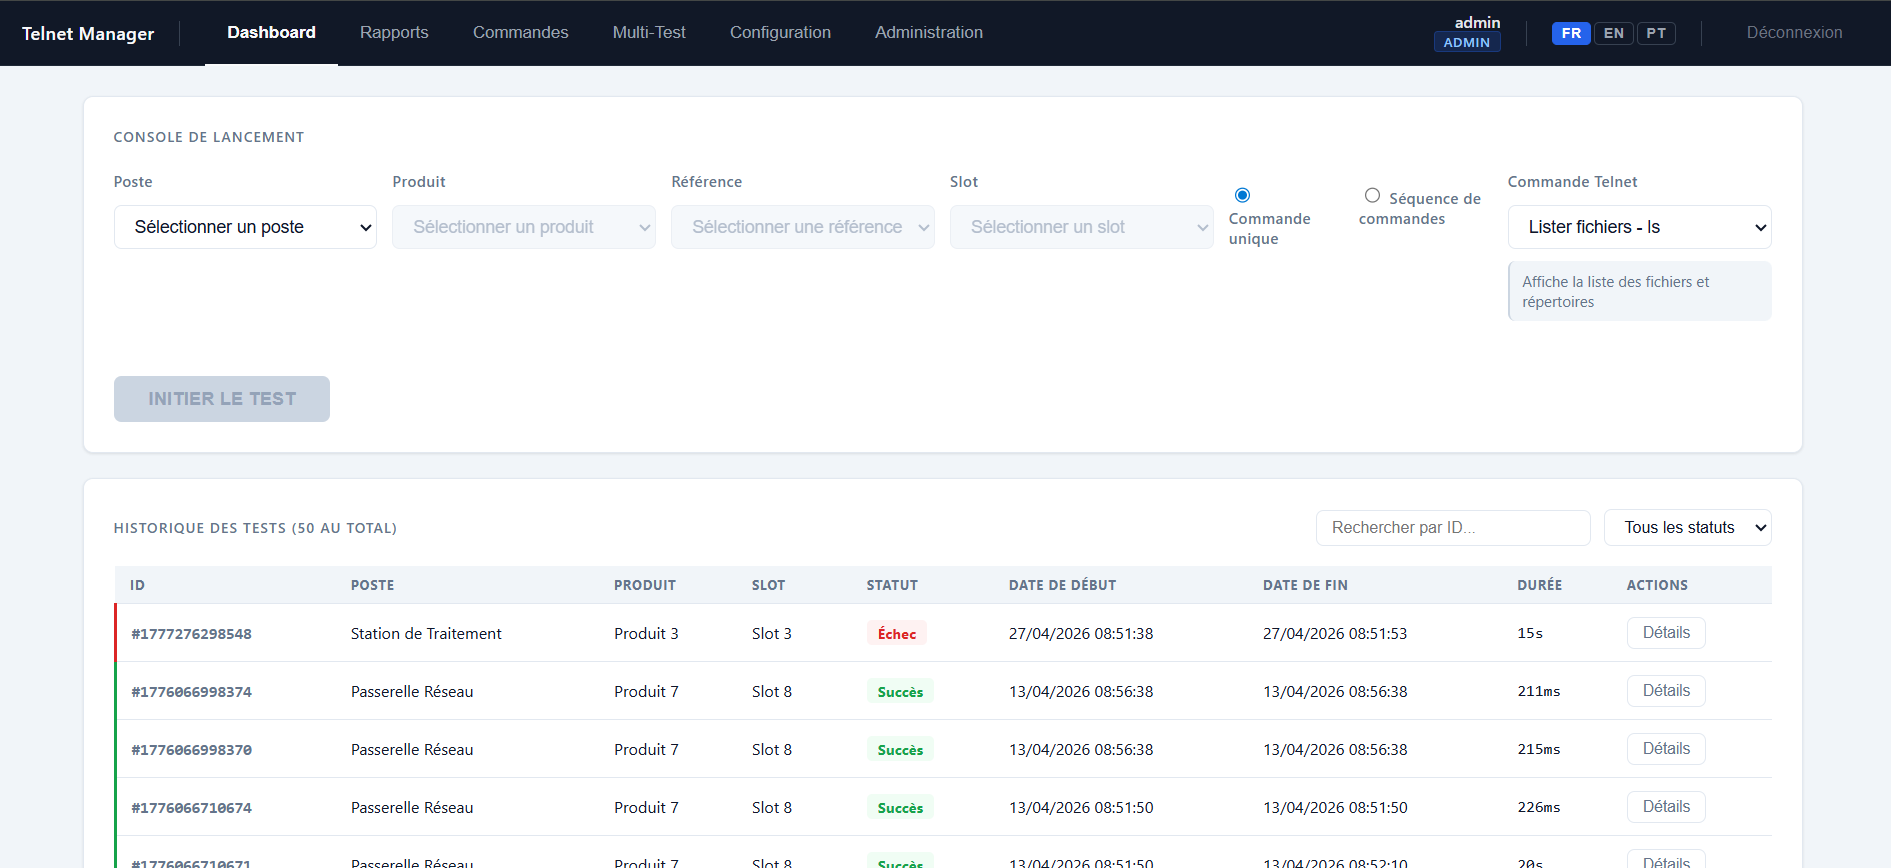
\includegraphics[width=\textwidth]{images/screen_dashboard}
  \caption{Capture d'écran~: Dashboard --- résultats en temps réel}
  \label{fig:screen_dashboard_live}
\end{figure}

\subsection{Gestion des équipements}

Le composant \texttt{Configuration.tsx} implémente la navigation
hiérarchique en onglets (Postes, Produits, Slots, Références). Chaque
onglet affiche un tableau paginé avec les opérations CRUD~:
\begin{itemize}
  \item \textbf{Ajouter}~: ouverture d'un formulaire modal avec
        validation côté client~;
  \item \textbf{Modifier}~: pré-remplissage du formulaire avec les
        données existantes~;
  \item \textbf{Supprimer}~: confirmation avant envoi de
        \texttt{DELETE /\{resource\}/:id}.
\end{itemize}

\begin{figure}[H]
  \centering
  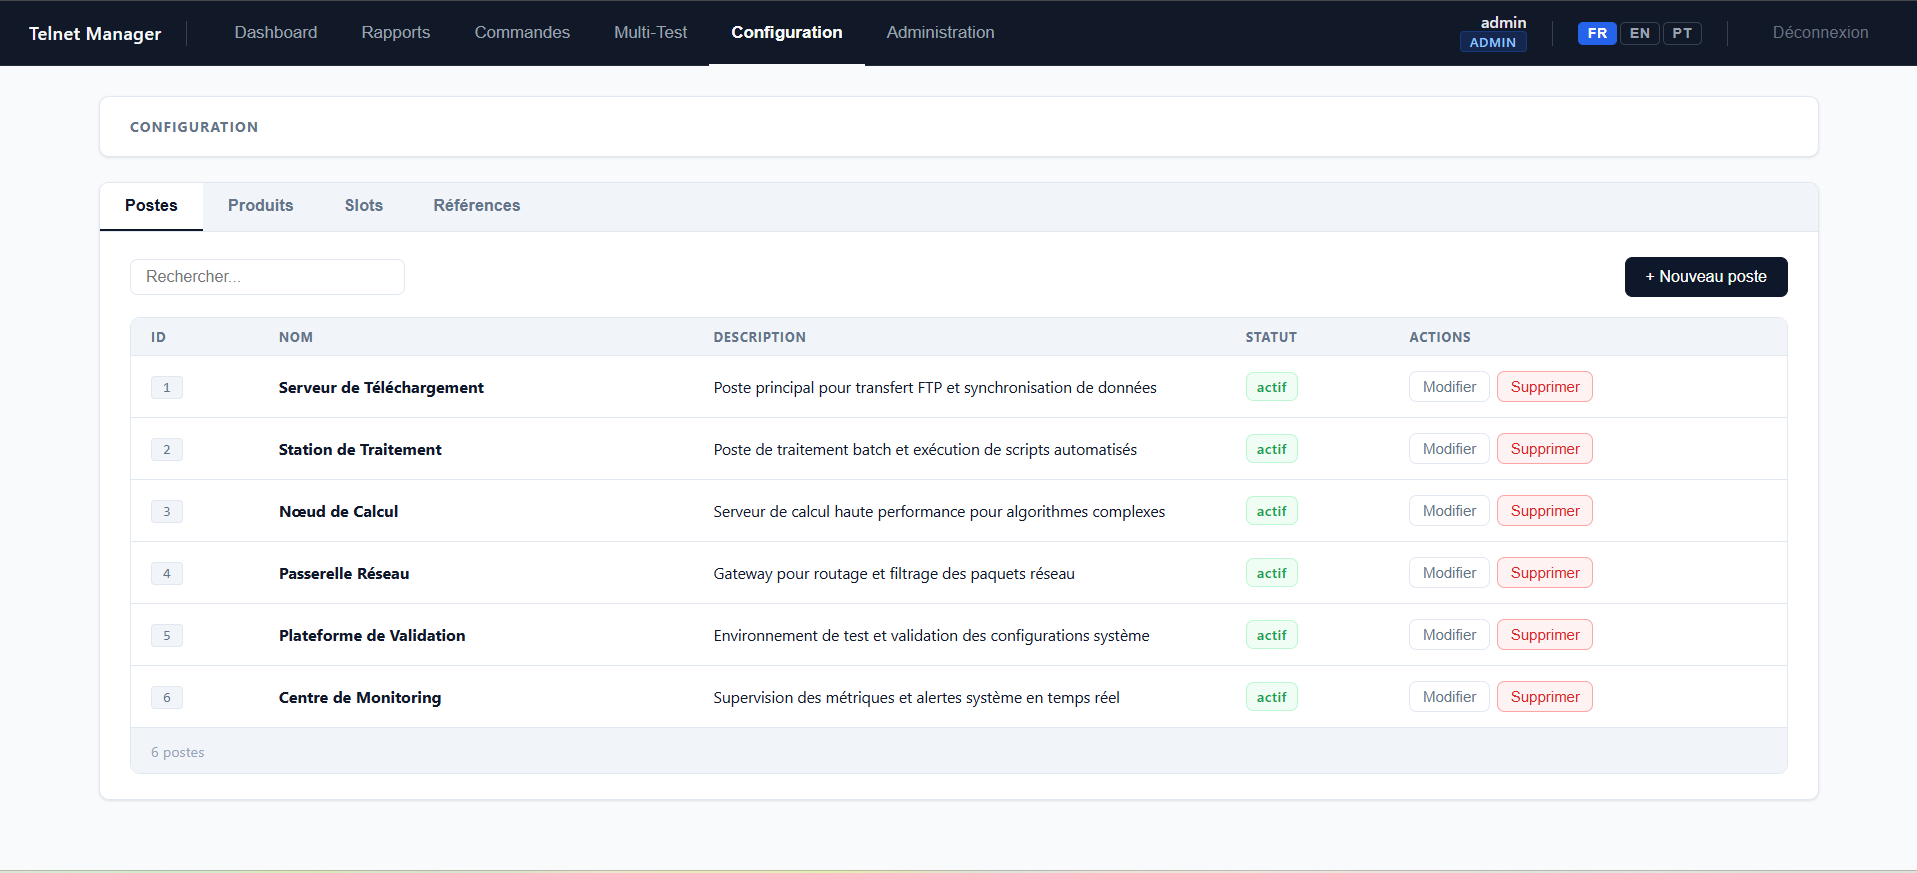
\includegraphics[width=\textwidth]{images/screen_config}
  \caption{Capture d'écran~: module de configuration --- gestion des slots}
  \label{fig:screen_config_slots}
\end{figure}

\subsection{Monitoring temps réel}

Le composant \texttt{MultiTest.tsx} permet de sélectionner plusieurs
slots et de lancer des tests Telnet en parallèle. Chaque slot a son
propre terminal de résultats, mis à jour indépendamment via les
messages WebSocket.

\begin{figure}[H]
  \centering
  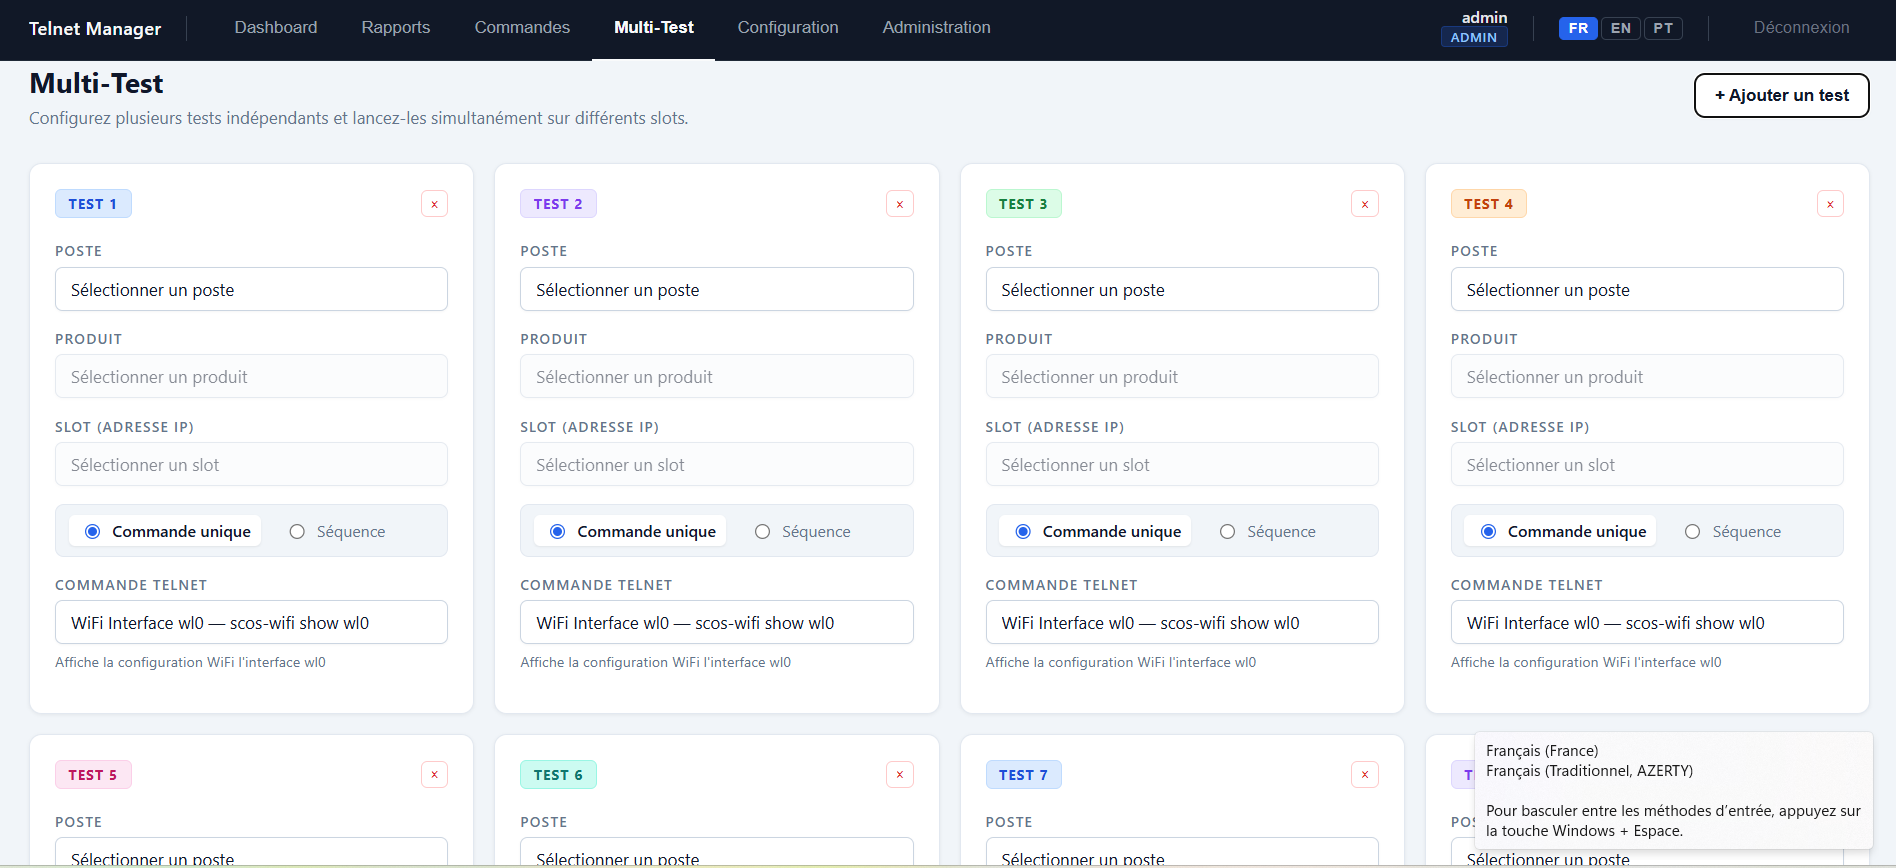
\includegraphics[width=\textwidth]{images/screen_multitest}
  \caption{Capture d'écran~: module MultiTest --- tests multi-slots en parallèle}
  \label{fig:screen_multitest_live}
\end{figure}

% -----------------------------------------------------------------
\section{Captures d'écran et démonstration}
% -----------------------------------------------------------------

\begin{figure}[H]
  \centering
  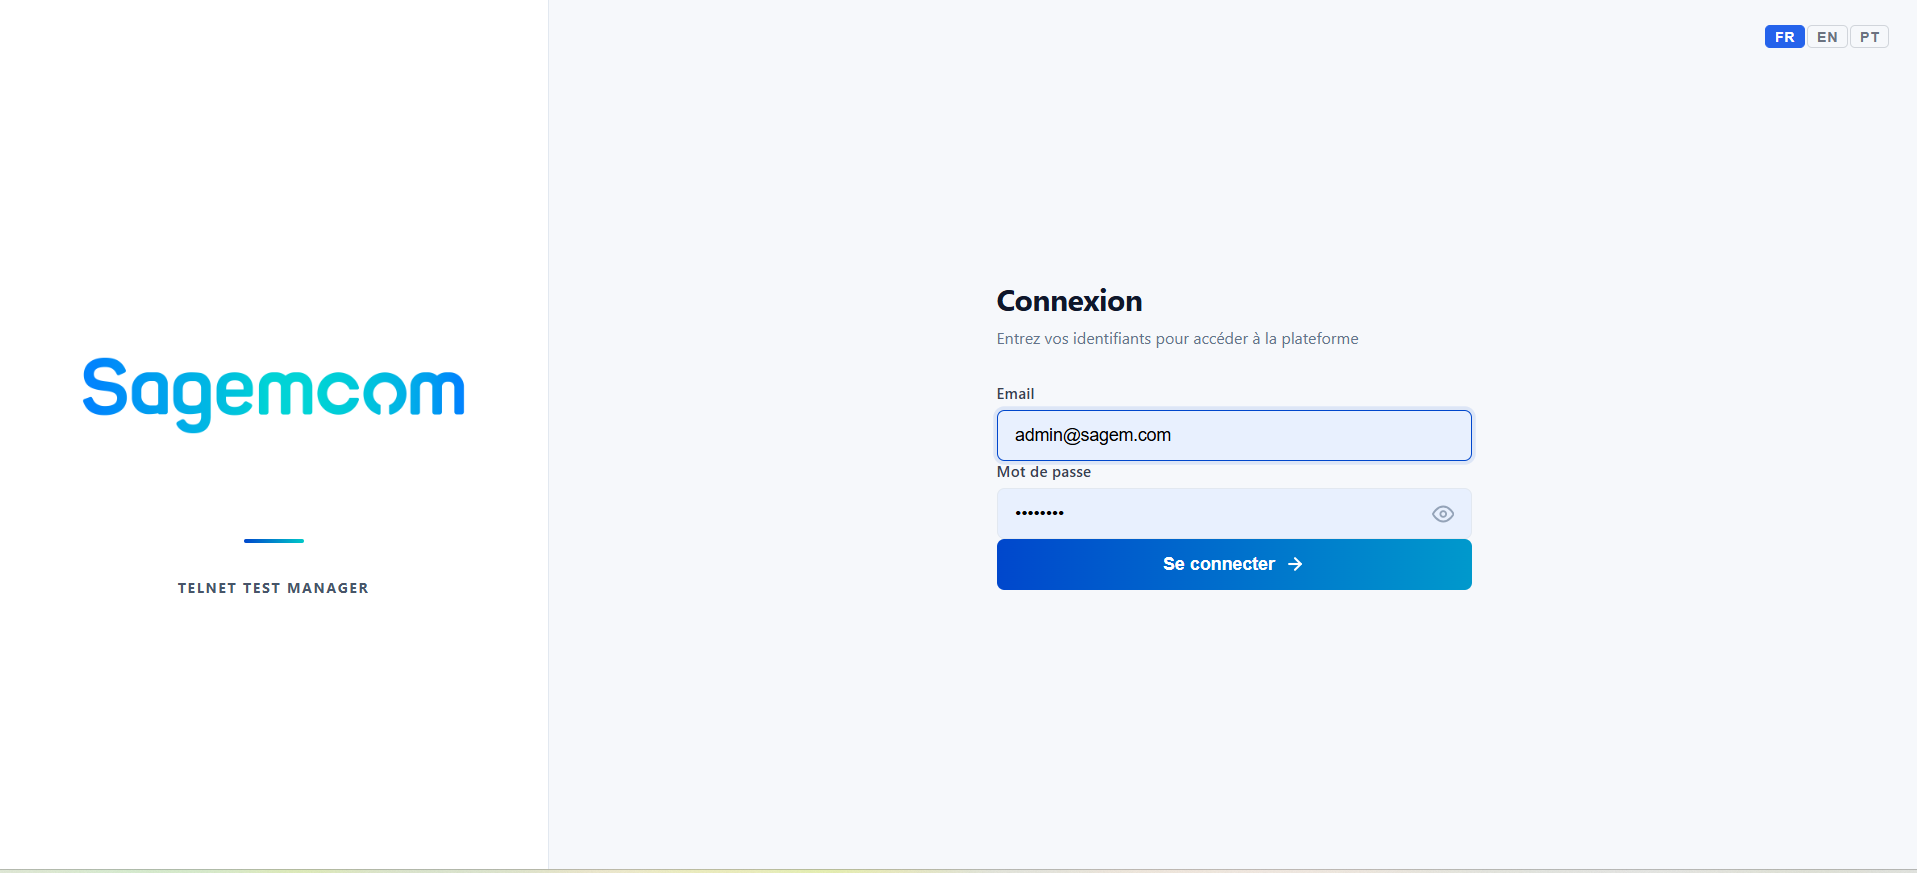
\includegraphics[width=0.75\textwidth]{images/screen_login}
  \caption{Capture d'écran~: interface d'authentification}
  \label{fig:screen_login}
\end{figure}

\begin{figure}[H]
  \centering
  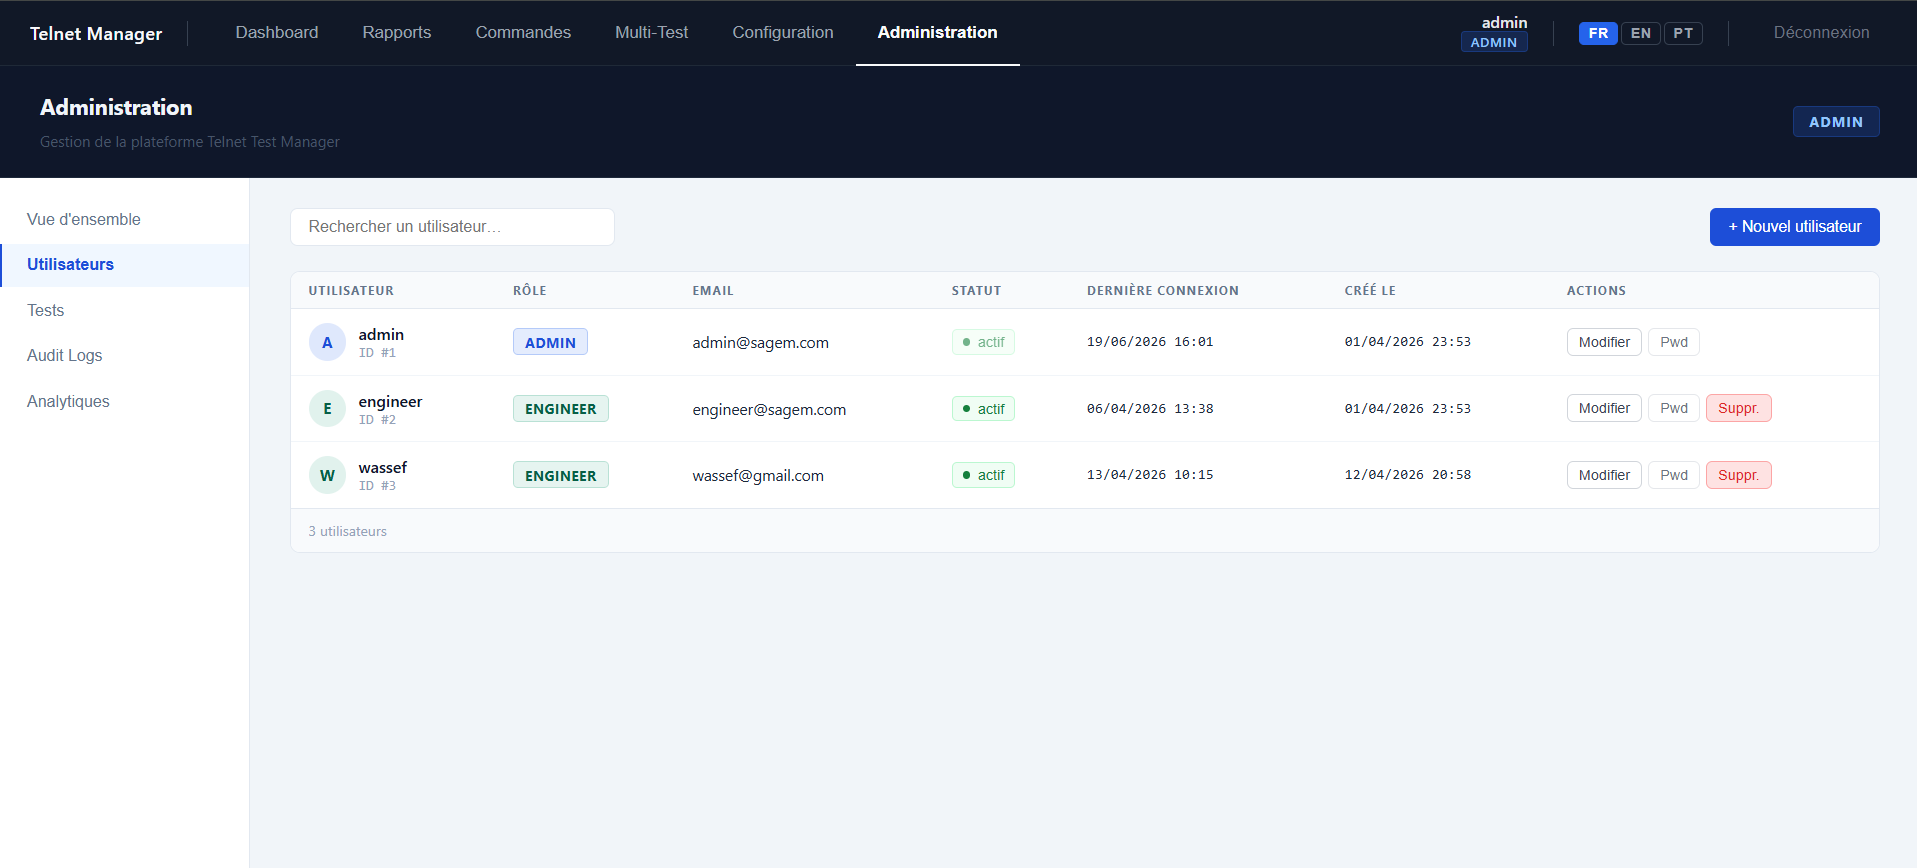
\includegraphics[width=\textwidth]{images/screen_admin}
  \caption{Capture d'écran~: panneau d'administration --- gestion des utilisateurs}
  \label{fig:screen_admin}
\end{figure}

\begin{figure}[H]
  \centering
  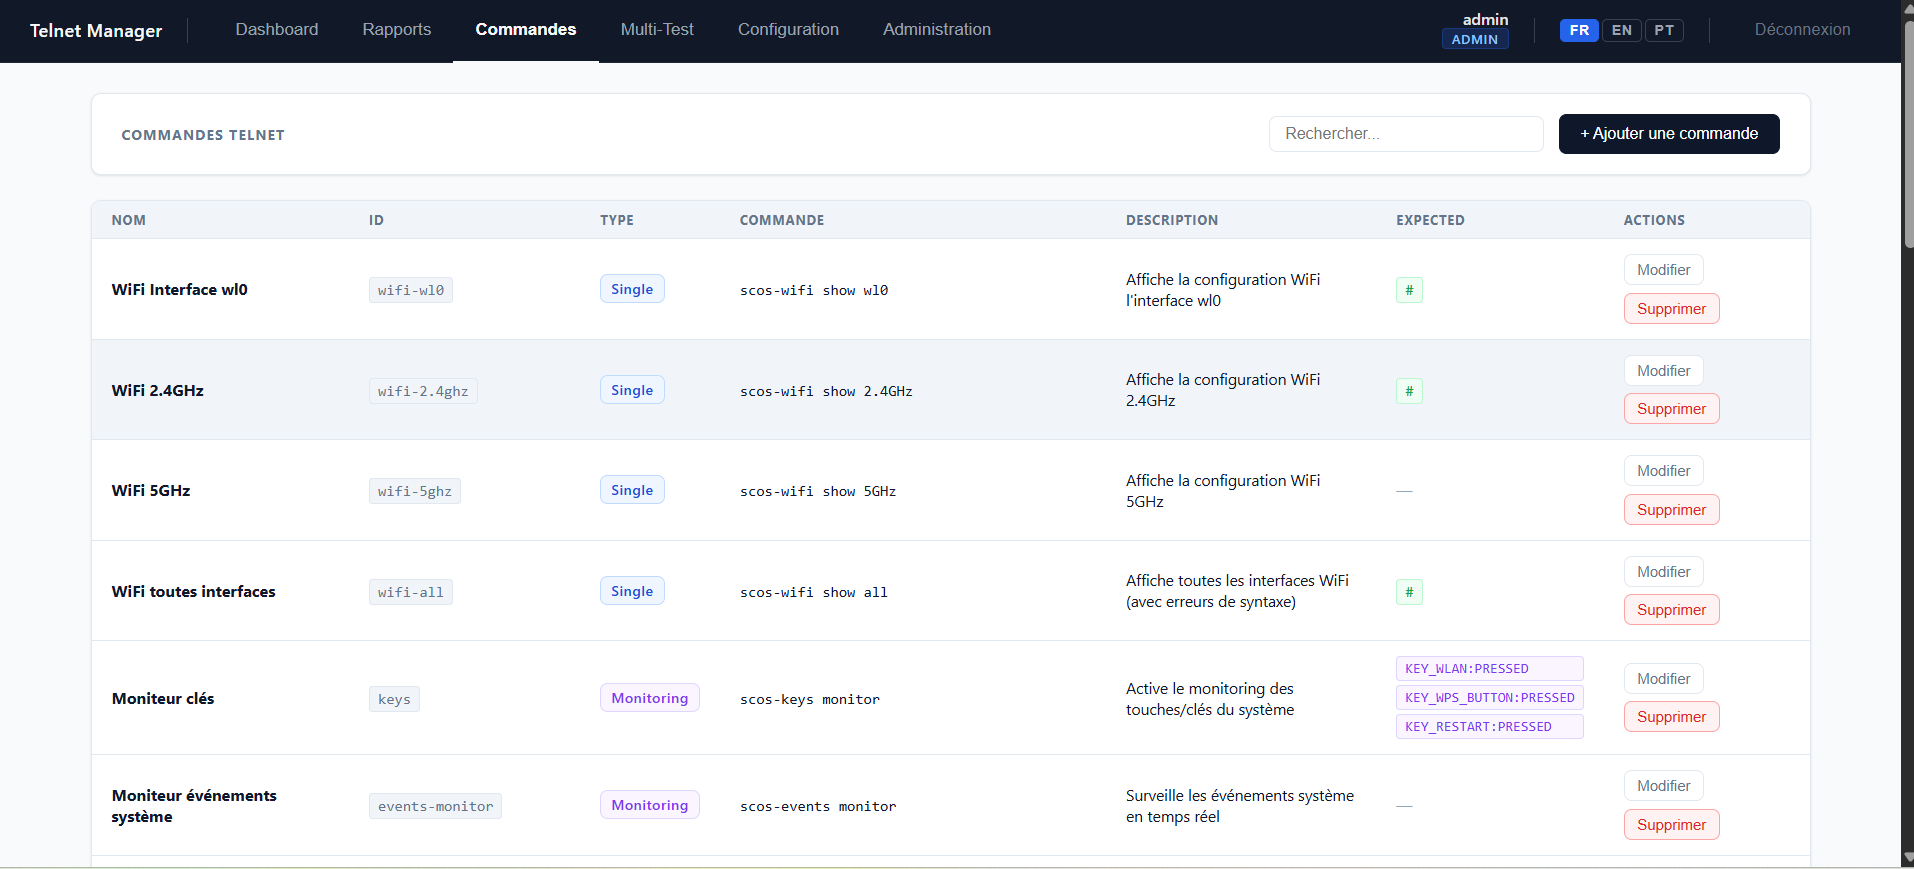
\includegraphics[width=\textwidth]{images/screen_commands}
  \caption{Capture d'écran~: bibliothèque de commandes Telnet}
  \label{fig:screen_commands}
\end{figure}

\begin{figure}[H]
  \centering
  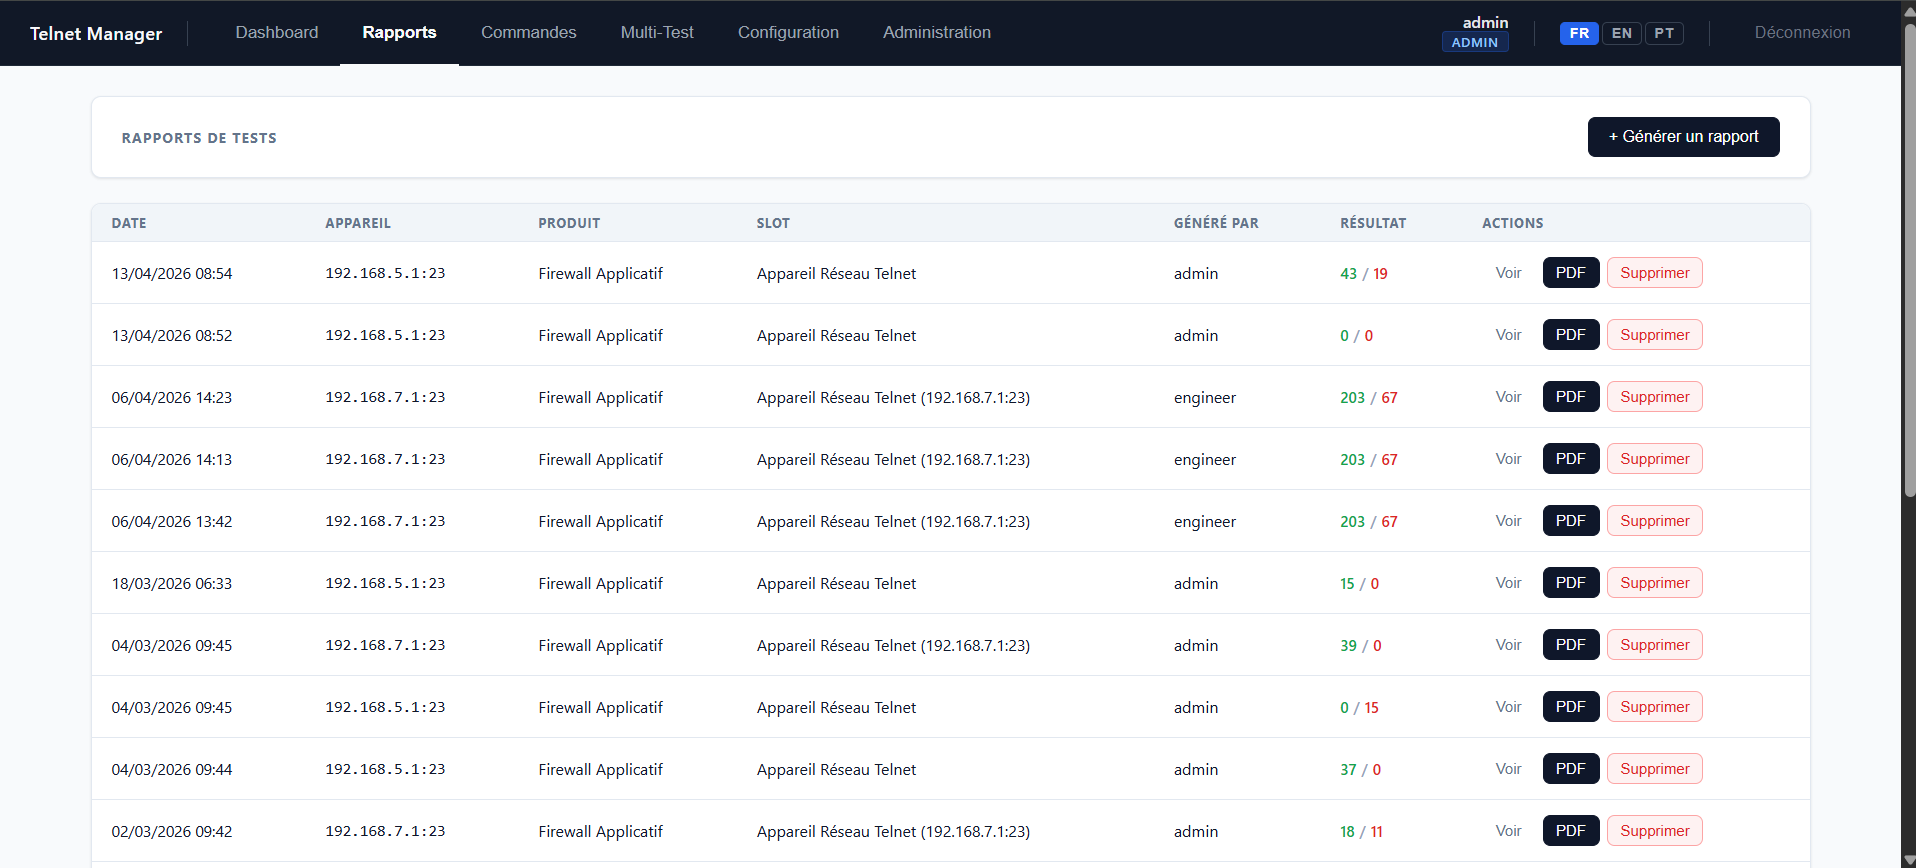
\includegraphics[width=\textwidth]{images/screen_reports}
  \caption{Capture d'écran~: module de génération de rapports}
  \label{fig:screen_reports}
\end{figure}

\begin{figure}[H]
  \centering
  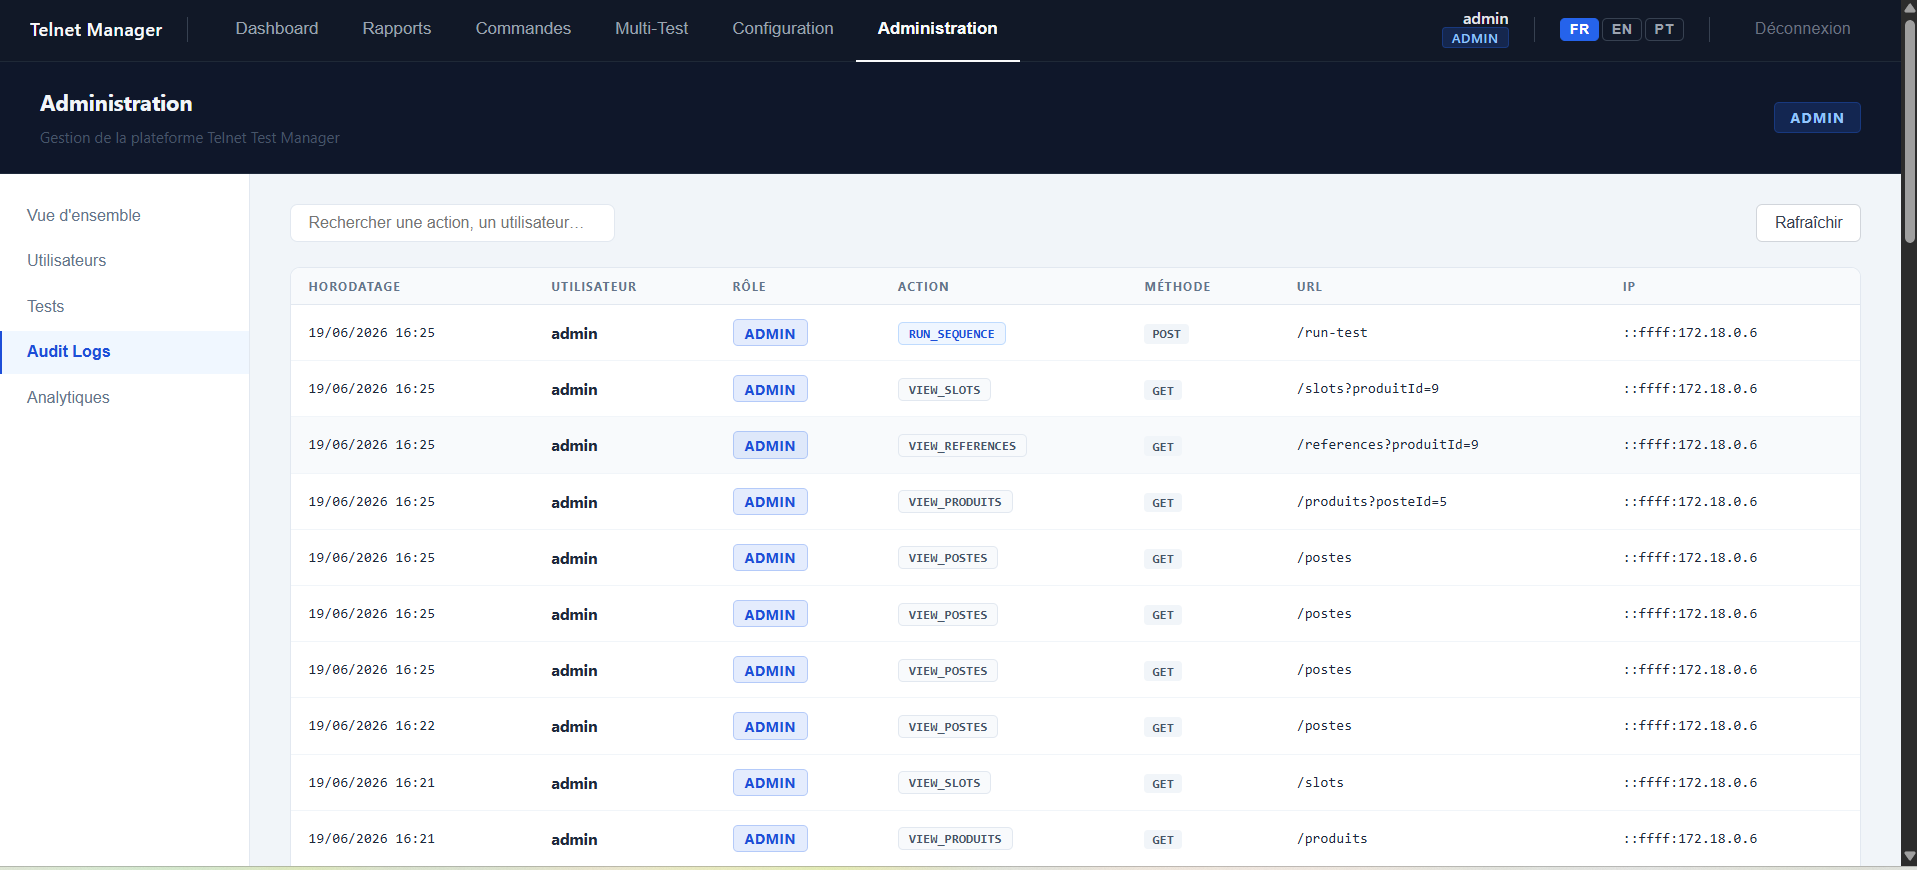
\includegraphics[width=\textwidth]{images/screen_auditlog}
  \caption{Capture d'écran~: journal d'audit --- traçabilité des actions utilisateurs}
  \label{fig:screen_auditlog}
\end{figure}

\section*{Conclusion}

Ce chapitre a couvert le développement des composants principaux de
Telnet Test Manager. Le moteur Telnet basé sur les Worker Threads assure
le non-blocage et le parallélisme. La Clean Architecture maintient une
séparation nette des responsabilités. Les 32 endpoints REST et la
connexion MongoDB forment la base de l'application. Le chapitre suivant
traite du déploiement et de l'infrastructure DevOps.

% =============================================================
%  Chapitre 5 — DevOps et déploiement
% =============================================================
\chapter{DevOps et déploiement}

\section*{Introduction}
Ce chapitre couvre toute la chaîne de livraison du projet~: de la
conteneurisation Docker à l'orchestration Kubernetes/Helm, en passant
par le pipeline GitHub Actions et la supervision Prometheus/Grafana.

% -----------------------------------------------------------------
\section{Introduction au DevOps et au CI/CD}
% -----------------------------------------------------------------

\textbf{DevOps} désigne un ensemble de pratiques qui rapprochent les
équipes de développement (Dev) et d'exploitation (Ops) pour accélérer
la livraison de logiciels fiables. Les trois axes principaux sont~:

\begin{itemize}
  \item \textbf{L'intégration continue (CI)}~: chaque poussée de code
        déclenche automatiquement la vérification, la compilation et les
        tests du projet~;
  \item \textbf{La livraison continue (CD)}~: le code validé est packagé
        et livré automatiquement sur l'environnement cible~;
  \item \textbf{Le monitoring}~: l'application déployée est surveillée en
        permanence pour détecter anomalies et dégradations de performance.
\end{itemize}

% -----------------------------------------------------------------
\section{Architecture DevOps du projet}
% -----------------------------------------------------------------

\begin{figure}[H]
  \centering
  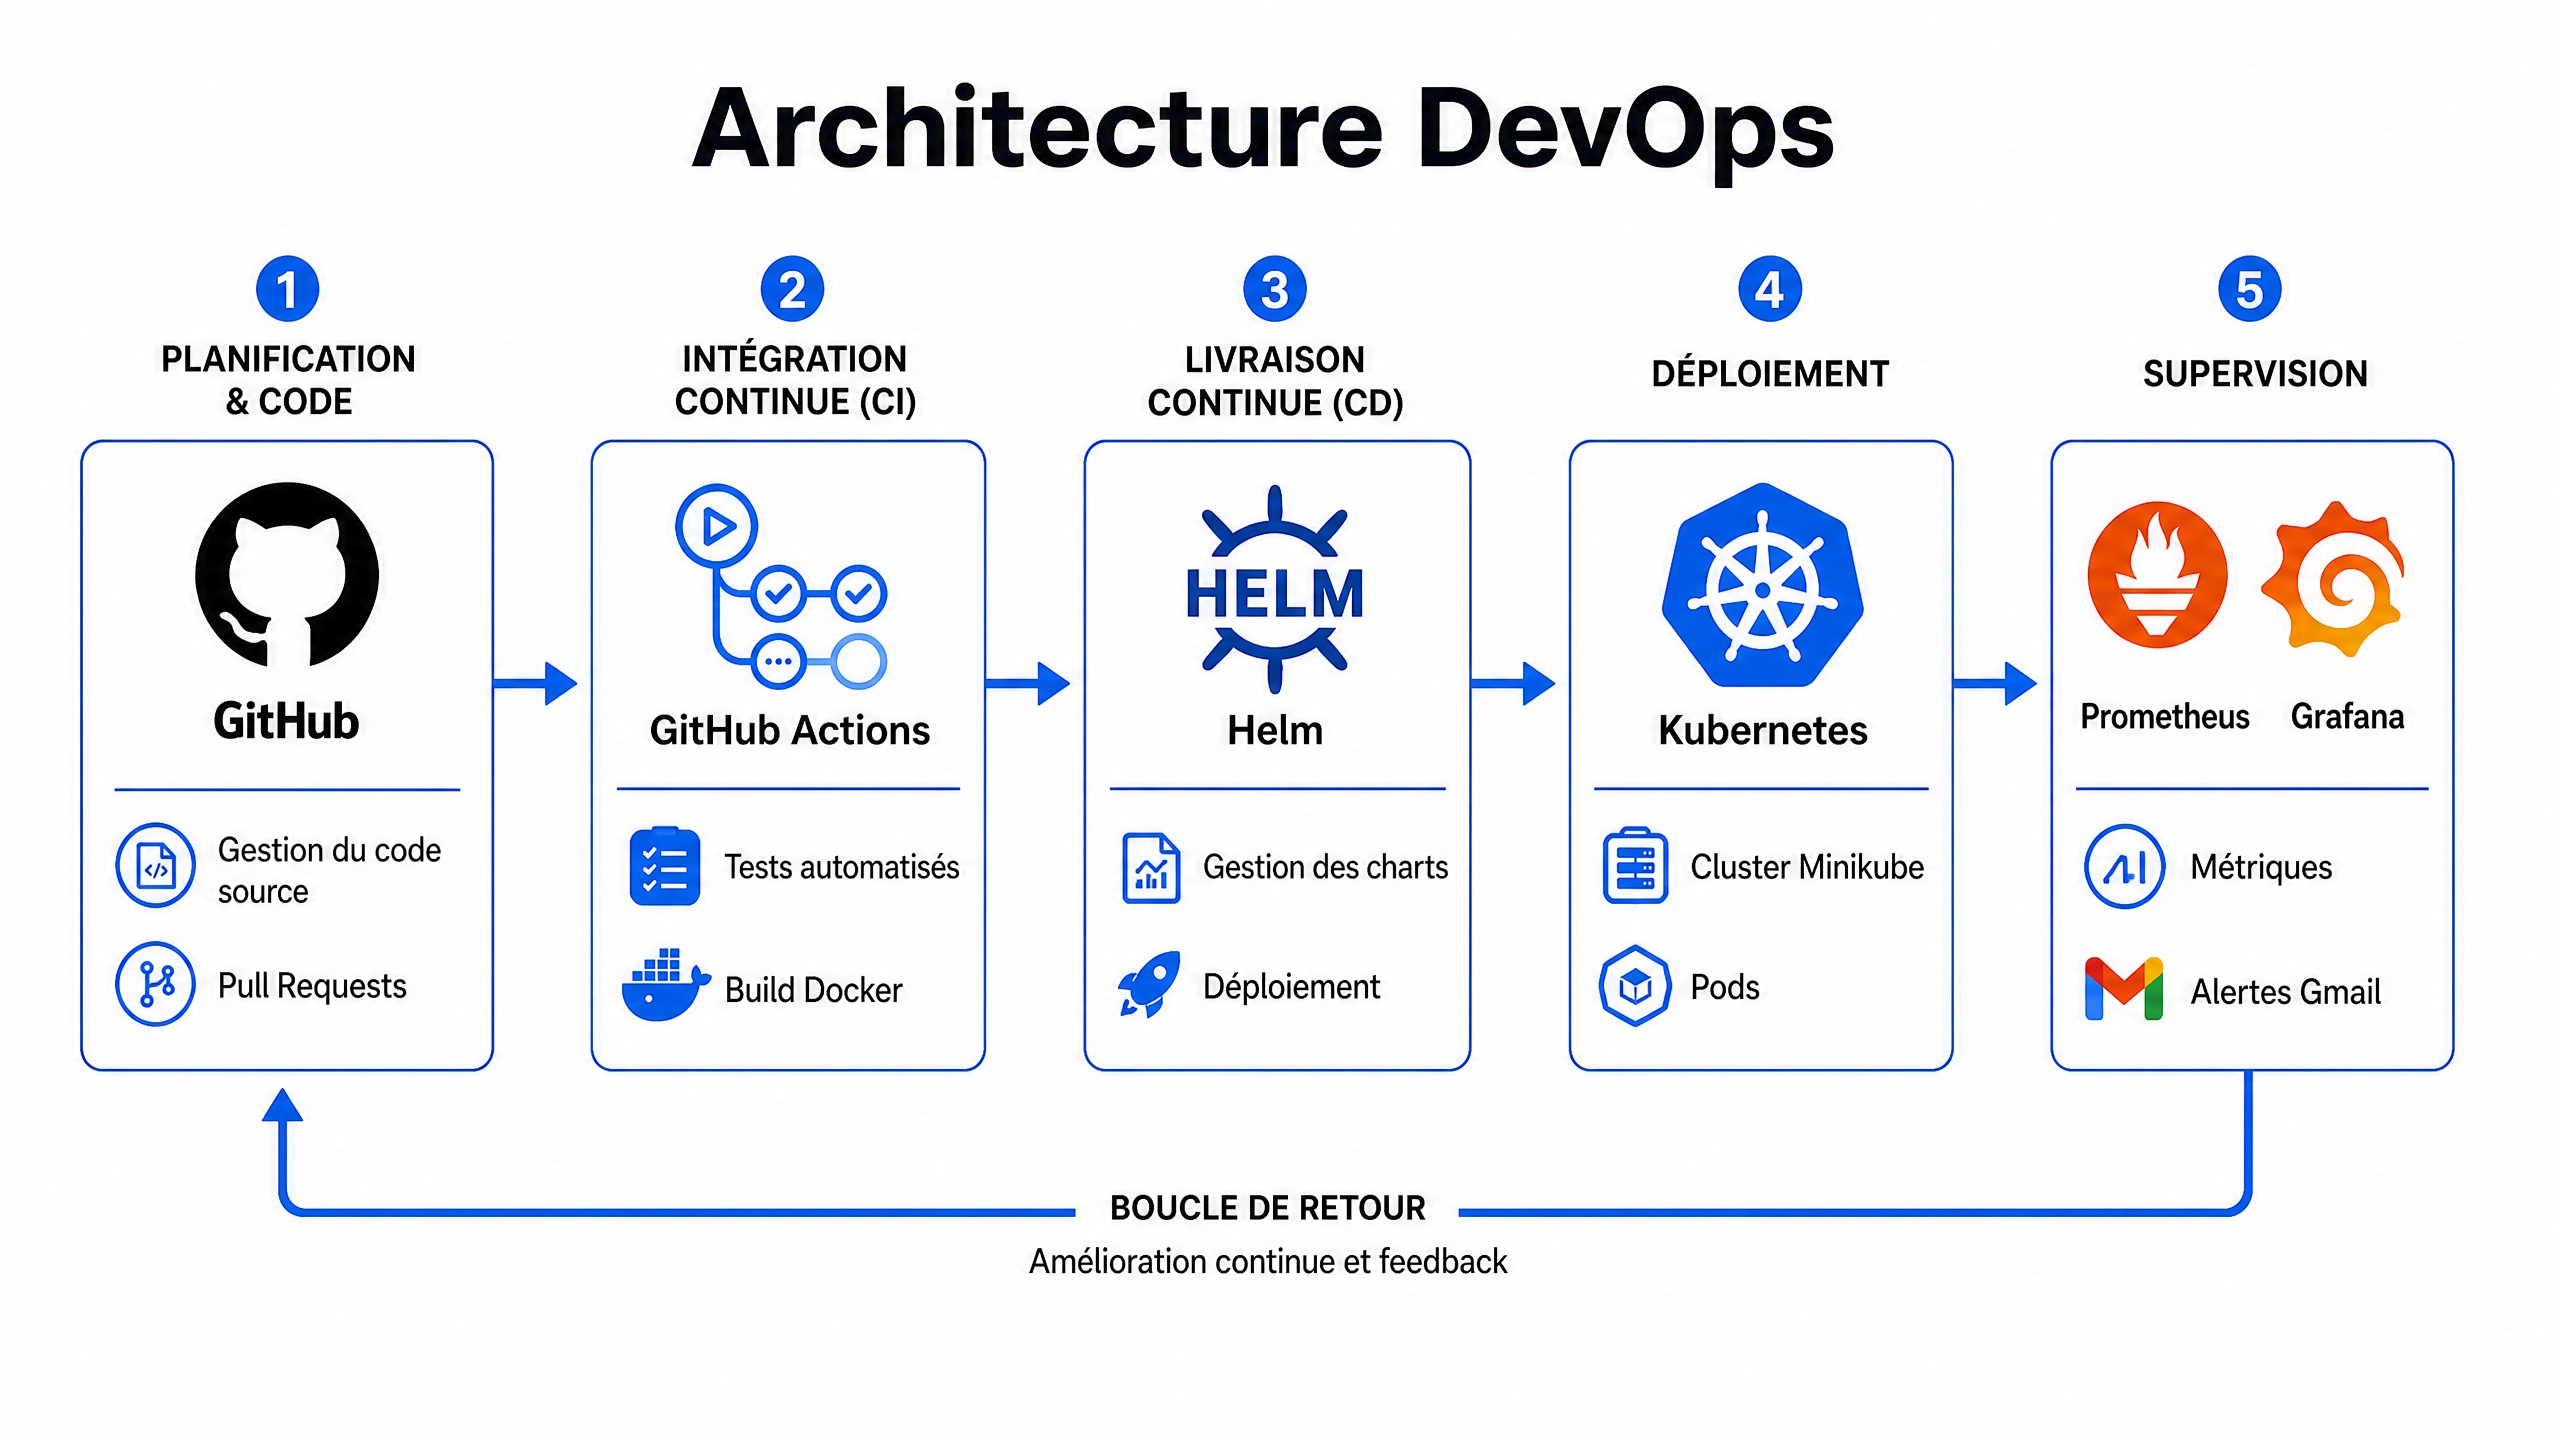
\includegraphics[width=\textwidth]{images/architecture_devops}
  \caption{Architecture DevOps — pipeline CI/CD et infrastructure Kubernetes}
  \label{fig:devops_archi}
\end{figure}

% -----------------------------------------------------------------
\section{Conteneurisation avec Docker}
% -----------------------------------------------------------------

\subsection{Dockerfile du backend}

Le \texttt{Dockerfile} du backend part de l'image \texttt{node:20-alpine},
une base Node.js 20 LTS légère sur Alpine Linux ($\sim$50~Mo). Les
dépendances sont installées avec \texttt{npm ci --only=production} pour
ne pas embarquer les outils de développement. Un argument \texttt{CACHEBUST}
force la re-copie du code source à chaque déploiement. L'application
écoute sur le port 3002 et démarre via \texttt{node src/main/server.js}.

\subsection{Dockerfile du frontend (multi-stage)}

Le \texttt{Dockerfile} du frontend exploite un build \textbf{multi-stage}~:
la première étape utilise \texttt{node:18-alpine} pour compiler l'application
React (\texttt{npm run build}), produisant les fichiers statiques optimisés.
La seconde étape repart d'une image \texttt{nginx:alpine} vierge et y copie
uniquement les fichiers compilés ainsi que la configuration Nginx (reverse proxy).
Cette approche ramène l'image finale de $\sim$900~Mo (avec les dépendances de build)
à $\sim$25~Mo en production.


\subsection{Docker Compose pour le développement}

Le fichier \texttt{docker-compose.yml} orchestre cinq services interdépendants~:
\begin{itemize}
  \item \textbf{mongodb}~: image \texttt{mongo:7} avec volume persistant
        \texttt{mongo-data} et variables d'environnement pour l'initialisation
        de la base~;
  \item \textbf{backend}~: expose les ports 3002 (API REST) et 3003 (WebSocket),
        reçoit la chaîne de connexion MongoDB et le secret JWT via des variables
        d'environnement~;
  \item \textbf{frontend}~: expose le port 3000, dépend du backend~;
  \item \textbf{prometheus}~: image officielle \texttt{prom/prometheus} avec le
        fichier de configuration scrape monté en volume~;
  \item \textbf{grafana}~: image officielle avec datasources et dashboards
        provisionnés automatiquement au démarrage.
\end{itemize}

% -----------------------------------------------------------------
\section{Orchestration avec Kubernetes et Helm}
% -----------------------------------------------------------------

\subsection{Structure des manifestes Kubernetes}

\begin{figure}[H]
  \centering
  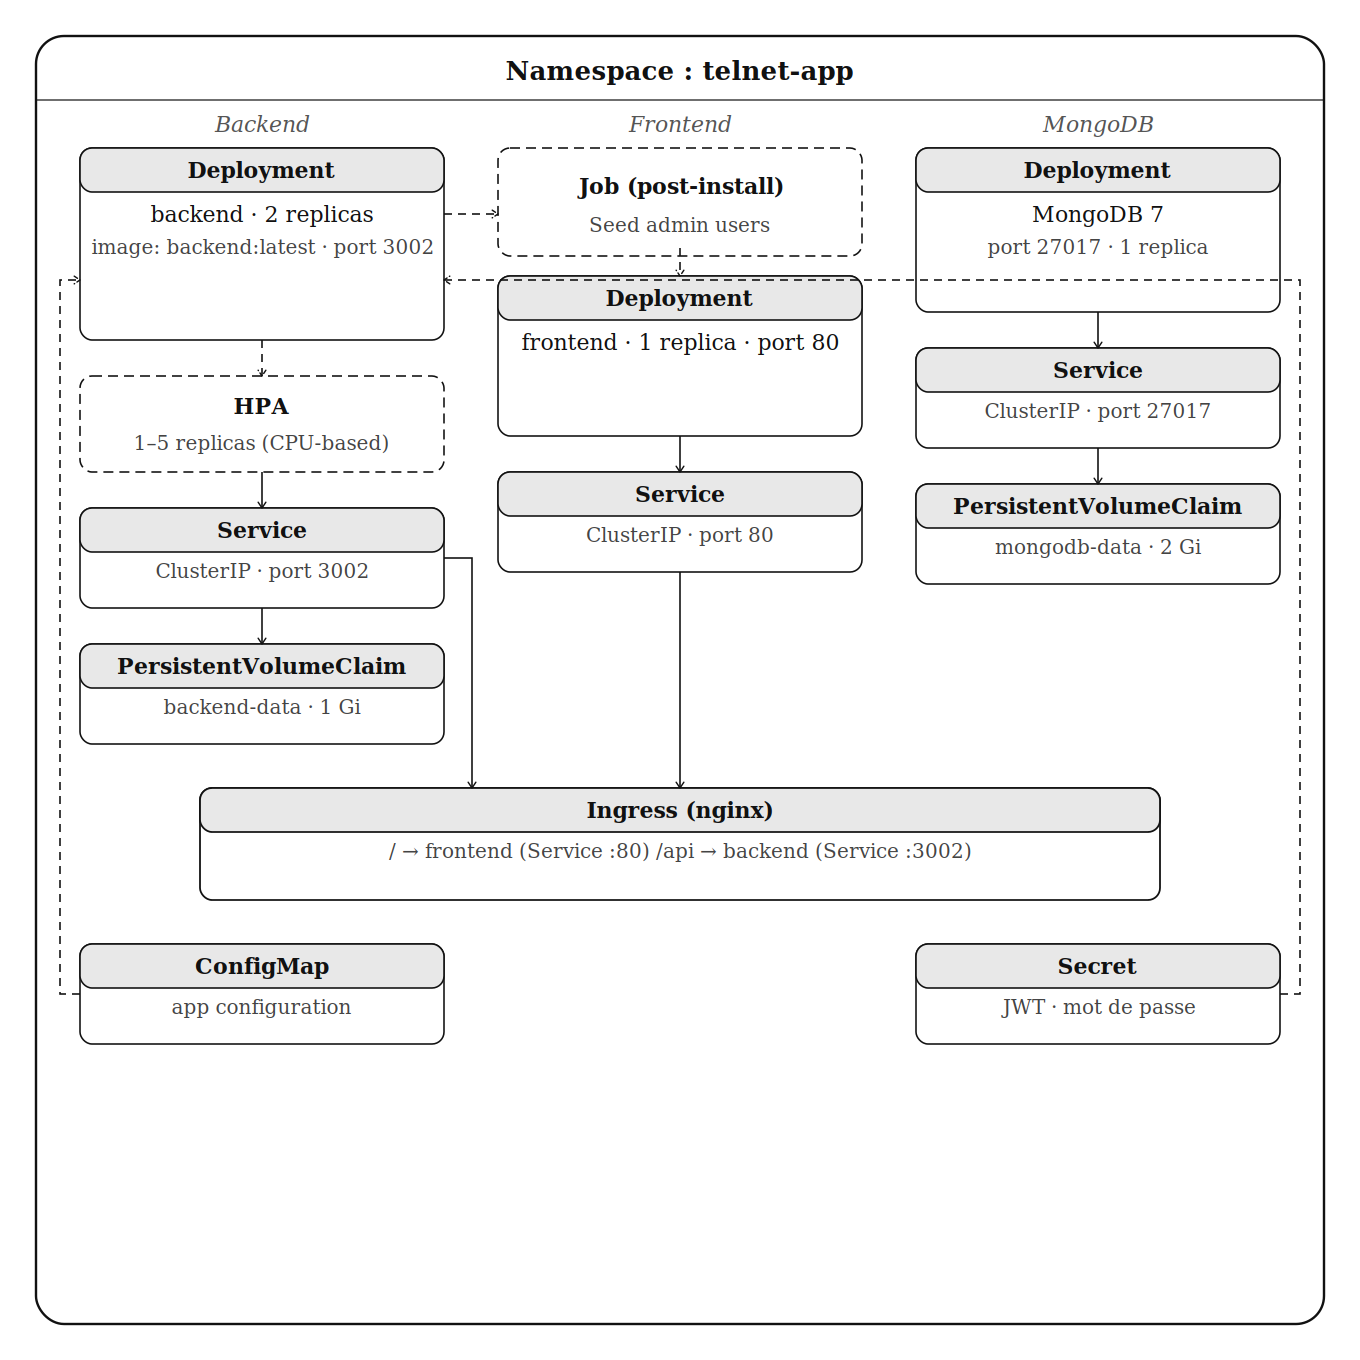
\includegraphics[width=\textwidth]{images/k8s_namespace_v2}
  \caption{Ressources Kubernetes déployées dans le namespace \texttt{telnet-app}}
  \label{fig:k8s_resources}
\end{figure}

\subsection{Chart Helm}

Le chart Helm \texttt{telnet-app} (version~0.3.0) paramétrise l'ensemble
des manifestes Kubernetes. Il comprend 12 templates et expose plus de
40 valeurs configurables dans \texttt{values.yaml}~:

Le fichier \texttt{values.yaml} expose plus de 40 paramètres configurables regroupés
par catégorie~: le nombre de répliques (\texttt{replicaCount}) pour chaque service,
les références d'images Docker (\texttt{image.backend}, \texttt{image.frontend},
\texttt{image.mongodb}), les ports de services, la configuration Ingress
(\texttt{telnet-app.local}), les tailles de volumes persistants (1~Gi pour le backend,
2~Gi pour MongoDB), les paramètres HPA (minReplicas~: 1, maxReplicas~: 5, seuil
CPU~: 70~\%) et les limites de ressources CPU/mémoire pour chaque conteneur.

\subsection{Horizontal Pod Autoscaler}

Le \textbf{HorizontalPodAutoscaler} (version \texttt{autoscaling/v2})
cible le Deployment du backend. Il ajuste automatiquement le nombre de
pods entre 1 et 5 dès que l'utilisation CPU moyenne dépasse 70~\%. Les
seuils (\texttt{minReplicas}, \texttt{maxReplicas} et
\texttt{targetCPUUtilizationPercentage}) sont définis dans
\texttt{values.yaml}, ce qui permet de les modifier sans toucher aux
templates Helm.

\begin{figure}[H]
  \centering
  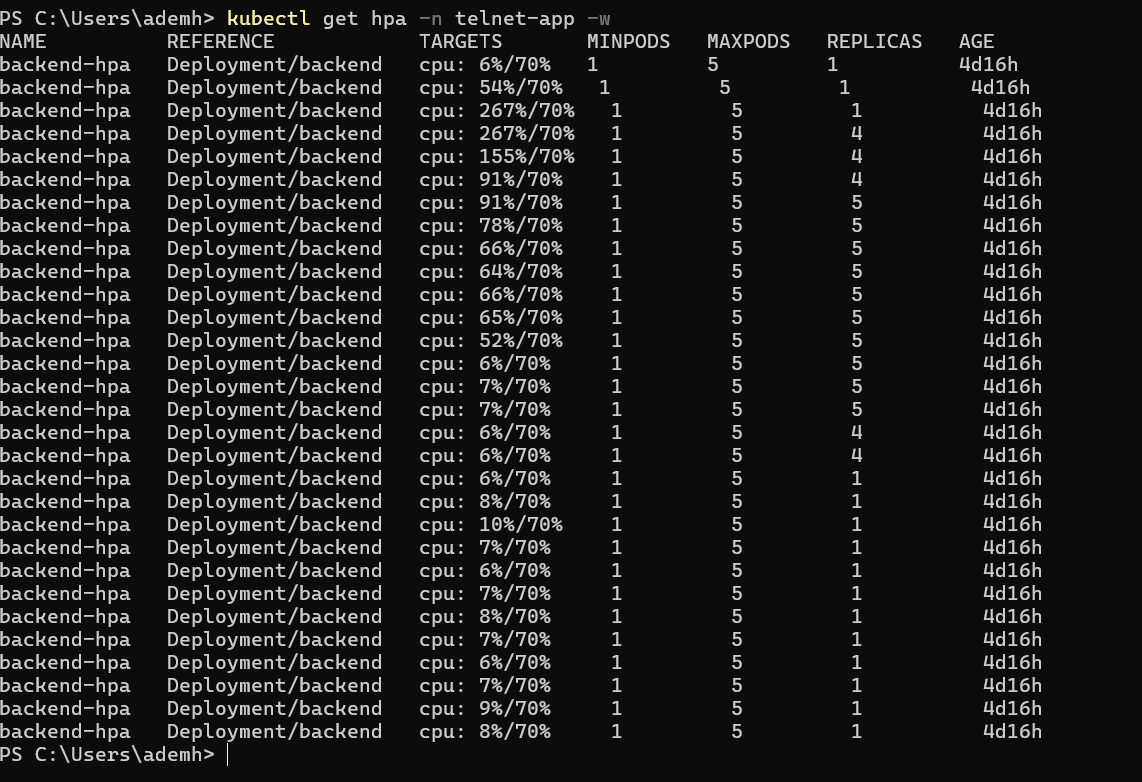
\includegraphics[width=\textwidth]{images/backend replicas after load test}
  \caption{Montée en charge HPA --- répliques backend passant de 1 à 5 sous stress CPU (267\,\%/70\,\%)}
  \label{fig:hpa_scaling}
\end{figure}

\subsection{Stratégie de déploiement Rolling Update}

Kubernetes utilise par défaut une stratégie de \textbf{rolling update}~:
les nouveaux pods démarrent progressivement pendant que les anciens
restent actifs, ce qui évite toute interruption de service.

Le Deployment backend est configuré avec \texttt{maxUnavailable~: 0} et
\texttt{maxSurge~: 1}. Concrètement, aucun pod n'est supprimé tant que
le nouveau n'est pas prêt, et un pod supplémentaire est autorisé pendant
la transition. Résultat~: les mises à jour se font en \textit{zero downtime}.

% -----------------------------------------------------------------
\section{Pipeline GitHub Actions}
% -----------------------------------------------------------------

\subsection{Vue d'ensemble du workflow}

Le workflow \texttt{ci-cd.yaml} se déclenche sur tout push vers \texttt{main} ou
\texttt{develop} et sur les pull requests vers \texttt{main}. Un mécanisme de
\texttt{concurrency} annule les exécutions précédentes de la même branche pour
éviter les déploiements en parallèle. Le pipeline comprend trois jobs~:

\begin{itemize}
  \item \textbf{ci-backend} (runner Ubuntu)~: installation des dépendances
        (\texttt{npm ci}), audit de sécurité (\texttt{npm audit --audit-level=critical})
        et exécution des tests unitaires~;
  \item \textbf{ci-frontend} (runner Ubuntu)~: mêmes étapes plus un build de
        production React (\texttt{npm run build})~;
  \item \textbf{deploy} (runner auto-hébergé, branche \texttt{main} uniquement)~:
        démarrage de Minikube si nécessaire, construction des images Docker dans le
        daemon Minikube, déploiement via \texttt{helm upgrade --install --atomic} avec
        injection des secrets depuis les variables GitHub Actions, puis attente du
        rollout avec \texttt{kubectl rollout status}.
\end{itemize}

À l'issue du déploiement, un résumé est automatiquement généré dans
l'interface GitHub Actions via \texttt{\$GITHUB\_STEP\_SUMMARY}~: il
récapitule le commit, la branche, l'heure de déploiement et l'état
des pods dans les namespaces \texttt{telnet-app} et \texttt{monitoring}.

\subsection{Configuration du runner auto-hébergé}

Le job \texttt{deploy} s'exécute sur un runner \textbf{auto-hébergé}
(\textit{self-hosted}) installé directement sur la machine Windows locale
hébergeant Minikube. Cette configuration est nécessaire car~:
\begin{itemize}
  \item L'accès au cluster Minikube est local et non exposé sur Internet~;
  \item Les images Docker doivent être construites dans le daemon Docker
        de Minikube (sans registry externe)~;
  \item Les secrets d'infrastructure restent dans l'environnement local.
\end{itemize}

Le runner est enregistré sur GitHub via~:
L'enregistrement du runner s'effectue en deux commandes~: \texttt{config.cmd}
reçoit l'URL du dépôt, un token d'authentification éphémère et les labels
(\texttt{self-hosted}, \texttt{windows}, \texttt{minikube}) qui permettent au
job \texttt{deploy} de le cibler. La commande \texttt{run.cmd} démarre ensuite
le runner en écoute permanente des jobs GitHub Actions.

% -----------------------------------------------------------------
\section{Supervision avec Prometheus et Grafana}
% -----------------------------------------------------------------

\subsection{Métriques Prometheus}

Quatre métriques personnalisées sont exposées sur \texttt{/metrics}~:

\begin{table}[H]
  \centering
  \caption{Métriques Prometheus de Telnet Test Manager}
  \label{tab:prometheus_metrics}
  \begin{tabularx}{\textwidth}{|L{6.2cm}|L{2.3cm}|X|}
    \hline
    \textbf{Métrique} & \textbf{Type} & \textbf{Description} \\
    \hline
    {\small\texttt{http\_requests\_total}} & Counter &
      Nombre total de requêtes HTTP par méthode, route et code de statut \\
    \hline
    {\small\texttt{http\_request\_duration\_seconds}} & Histogram &
      Distribution des temps de réponse par route (buckets~: 10\,ms à 5\,s) \\
    \hline
    {\small\texttt{telnet\_tests\_launched\_total}} & Counter &
      Nombre total de tests Telnet lancés \\
    \hline
    {\small\texttt{websocket\_active\_connections}} & Gauge &
      Nombre de connexions WebSocket actives en temps réel \\
    \hline
  \end{tabularx}
\end{table}

Le module \texttt{prometheusMetrics.js} active d'abord la collecte des métriques
par défaut de la VM Node.js via \texttt{collectDefaultMetrics} (CPU, mémoire, heap,
event loop). Il définit ensuite quatre métriques personnalisées~: un \texttt{Counter}
\texttt{http\_requests\_total} labellisé par méthode, route et code HTTP~; un
\texttt{Histogram} \texttt{http\_request\_duration\_seconds} avec 8 buckets de
10~ms à 5~s~; un \texttt{Counter} \texttt{telnet\_tests\_launched\_total} incrémenté
à chaque appel à \texttt{/run-test}~; et une \texttt{Gauge}
\texttt{websocket\_active\_connections} mise à jour à chaque connexion ou
déconnexion WebSocket.

\subsection{Tableau de bord Grafana}

Le tableau de bord \textbf{«~Telnet Test Manager~--- Monitoring~»} est
provisionné automatiquement au démarrage de Grafana via un fichier JSON.
Il comprend dix panneaux~:

\begin{table}[H]
  \centering
  \caption{Panneaux du tableau de bord Grafana}
  \label{tab:grafana_panels}
  \begin{tabularx}{\textwidth}{|L{4.5cm}|L{2.5cm}|X|}
    \hline
    \textbf{Panneau} & \textbf{Type} & \textbf{Requête PromQL} \\
    \hline
    Backend UP/DOWN & Stat &
      \texttt{up\{job="backend"\}} \\
    \hline
    Tests Telnet lancés & Stat &
      \texttt{telnet\_tests\_launched\_total} \\
    \hline
    Requêtes HTTP totales & Stat &
      \texttt{sum(http\_requests\_total)} \\
    \hline
    RAM Backend (Mo) & Stat &
      {\small\texttt{process\_resident\_memory\_bytes / 1024\^{}2}} \\
    \hline
    Taux de requêtes par route & Séries temp. &
      \texttt{rate(http\_requests\_total[1m])} \\
    \hline
    Durée p95 des requêtes & Séries temp. &
      {\small\texttt{histogram\_quantile(0.95,}}\newline
      {\small\texttt{rate(http\_request\_duration\_}}\newline
      {\small\texttt{seconds\_bucket[1m]))}} \\
    \hline
    Connexions WebSocket & Séries temp. &
      \texttt{websocket\_active\_connections} \\
    \hline
    CPU Backend (\%) & Jauge &
      {\small\texttt{rate(process\_cpu\_seconds\_total[1m])}}\newline
      {\small\texttt{* 100}} \\
    \hline
    Requêtes par code statut & Barres &
      {\small\texttt{sum by (status)}}\newline
      {\small\texttt{(http\_requests\_total)}} \\
    \hline
    Top 5 routes par latence & Tableau &
      {\small\texttt{avg by (route)}}\newline
      {\small\texttt{(http\_request\_duration\_seconds)}} \\
    \hline
  \end{tabularx}
\end{table}

Une règle d'alerte \textbf{Backend CPU High} est configurée~: lorsque
l'utilisation CPU dépasse le seuil de 70\,\%, Grafana envoie automatiquement
une notification par e-mail avec le niveau de sévérité \texttt{CRITICAL}.

\begin{figure}[H]
  \centering
  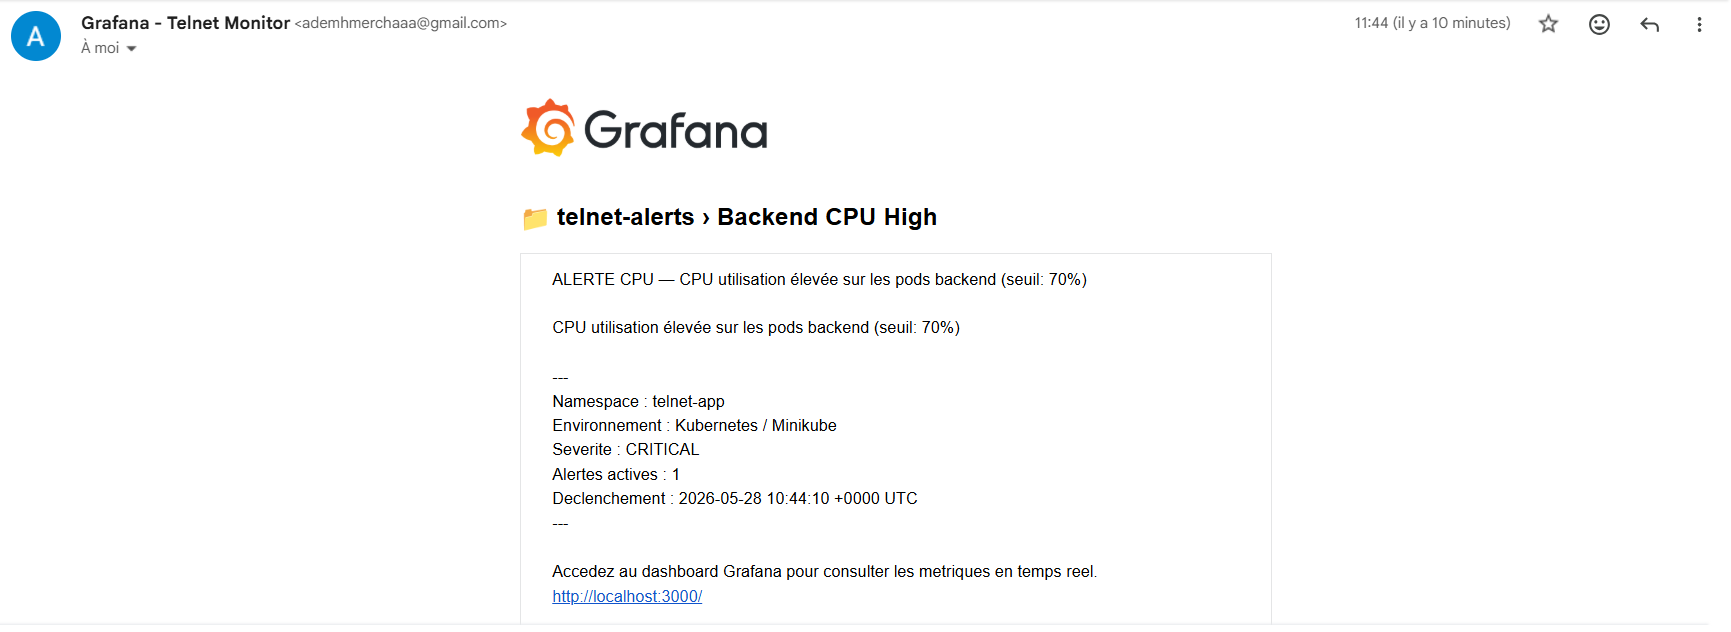
\includegraphics[width=0.85\textwidth]{images/grafana alert}
  \caption{Alerte e-mail Grafana --- déclenchement automatique sur dépassement CPU (seuil~: 70\,\%)}
  \label{fig:grafana_alert}
\end{figure}

% -----------------------------------------------------------------
\section{Infrastructure as Code}
% -----------------------------------------------------------------

L'\textbf{Infrastructure as Code} (IaC) consiste à gérer l'infrastructure
via des fichiers de configuration versionnés, comme on le ferait pour
du code applicatif. Ce projet l'applique à trois niveaux.

\subsection{Helm Charts}

Le chart Helm \texttt{telnet-app} (version~0.3.0) est la source unique
de vérité pour tout le déploiement Kubernetes. Il comprend 12 templates
paramétrables et expose plus de 40 valeurs configurables dans
\texttt{values.yaml}. Toute modification d'infrastructure (ressources,
répliques, secrets) passe par ce fichier versionné dans Git.

\begin{figure}[H]
  \centering
  \begin{lstlisting}[basicstyle=\ttfamily\small, frame=single, backgroundcolor=\color{gray!6}]
helm/telnet-app/
|-- Chart.yaml
|-- values.yaml
`-- templates/
    |-- backend-deployment.yaml
    |-- backend-service.yaml
    |-- backend-hpa.yaml
    |-- backend-pvc.yaml
    |-- frontend-deployment.yaml
    |-- frontend-service.yaml
    |-- mongodb-deployment.yaml
    |-- mongodb-service.yaml
    |-- mongodb-pvc.yaml
    |-- mongodb-initdb-configmap.yaml
    |-- configmap.yaml
    |-- secret.yaml
    |-- ingress.yaml
    `-- seed-job.yaml
  \end{lstlisting}
  \caption{Structure du chart Helm \texttt{telnet-app} --- 14 templates paramétrables}
  \label{fig:helm_structure}
\end{figure}

\subsection{Manifestes Kubernetes}

Chaque ressource Kubernetes est générée depuis le chart Helm~:
Deployments, Services, HPA, Ingress, PersistentVolumeClaims, ConfigMap
et Secrets. Les secrets applicatifs (mot de passe MongoDB, JWT secret,
SMTP) sont injectés via des variables de pipeline GitHub Actions
(\texttt{secrets.MONGO\_PASSWORD}, etc.) et ne sont jamais commités
dans le dépôt.

\begin{figure}[H]
  \centering
  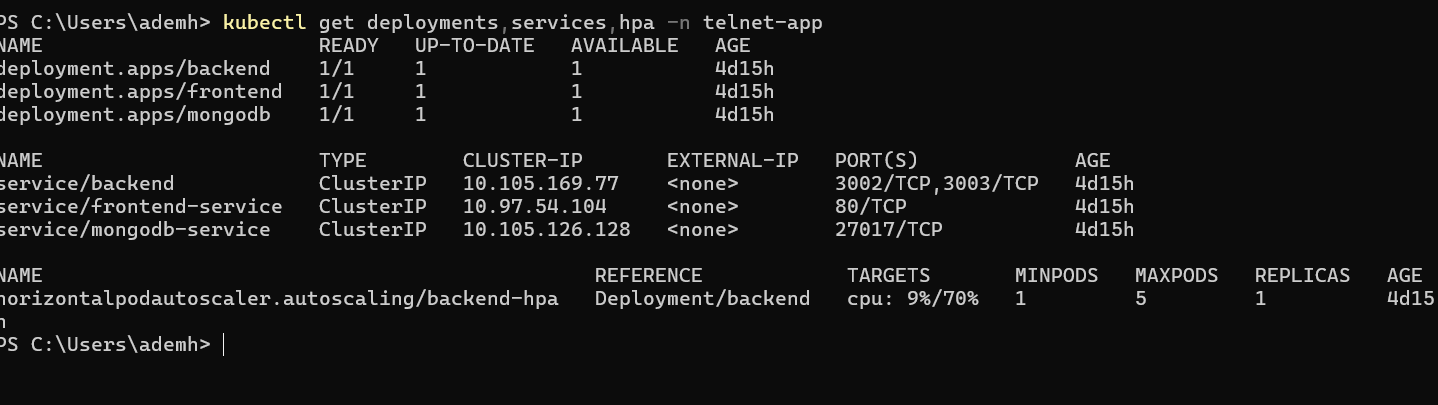
\includegraphics[width=\textwidth]{images/kubernetes deployements manifests}
  \caption{Ressources Kubernetes déployées dans le namespace \texttt{telnet-app}}
  \label{fig:kubectl_telnet}
\end{figure}

\begin{figure}[H]
  \centering
  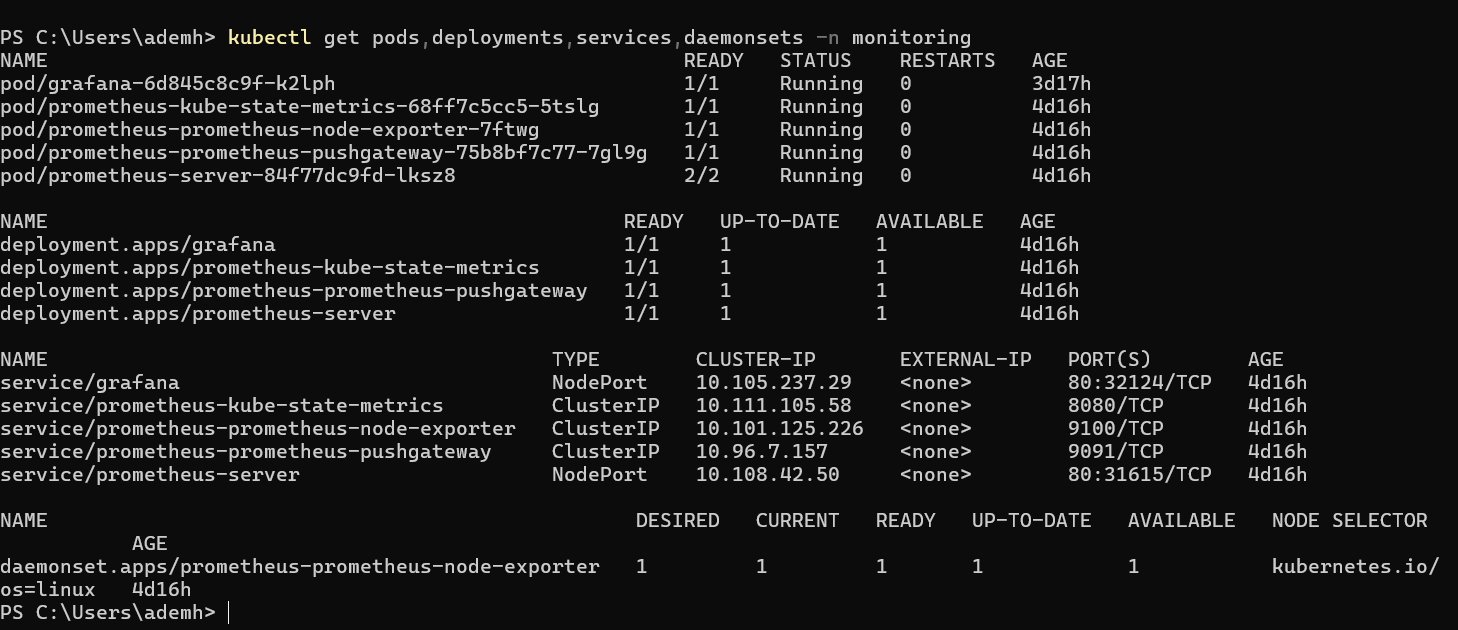
\includegraphics[width=\textwidth]{images/gafana_promethus manifeests}
  \caption{Ressources Kubernetes déployées dans le namespace \texttt{monitoring} (Prometheus et Grafana)}
  \label{fig:kubectl_monitoring}
\end{figure}

\subsection{Automatisation}

L'ensemble du cycle de vie de l'infrastructure est automatisé~:
\begin{itemize}
  \item \textbf{Provisioning}~: \texttt{helm upgrade --install} crée
        ou met à jour toutes les ressources de manière idempotente~;
  \item \textbf{Seeding}~: un Job Kubernetes post-install initialise
        les utilisateurs de démonstration en base MongoDB~;
  \item \textbf{Monitoring}~: Prometheus et Grafana sont déployés via
        leurs propres charts Helm avec dashboards et alertes provisionnés
        en code (\texttt{grafana-values.yaml})~;
  \item \textbf{Rollback}~: \texttt{helm rollback telnet-app}
        restaure en un seul appel la version précédente.
\end{itemize}

\begin{figure}[H]
  \centering
  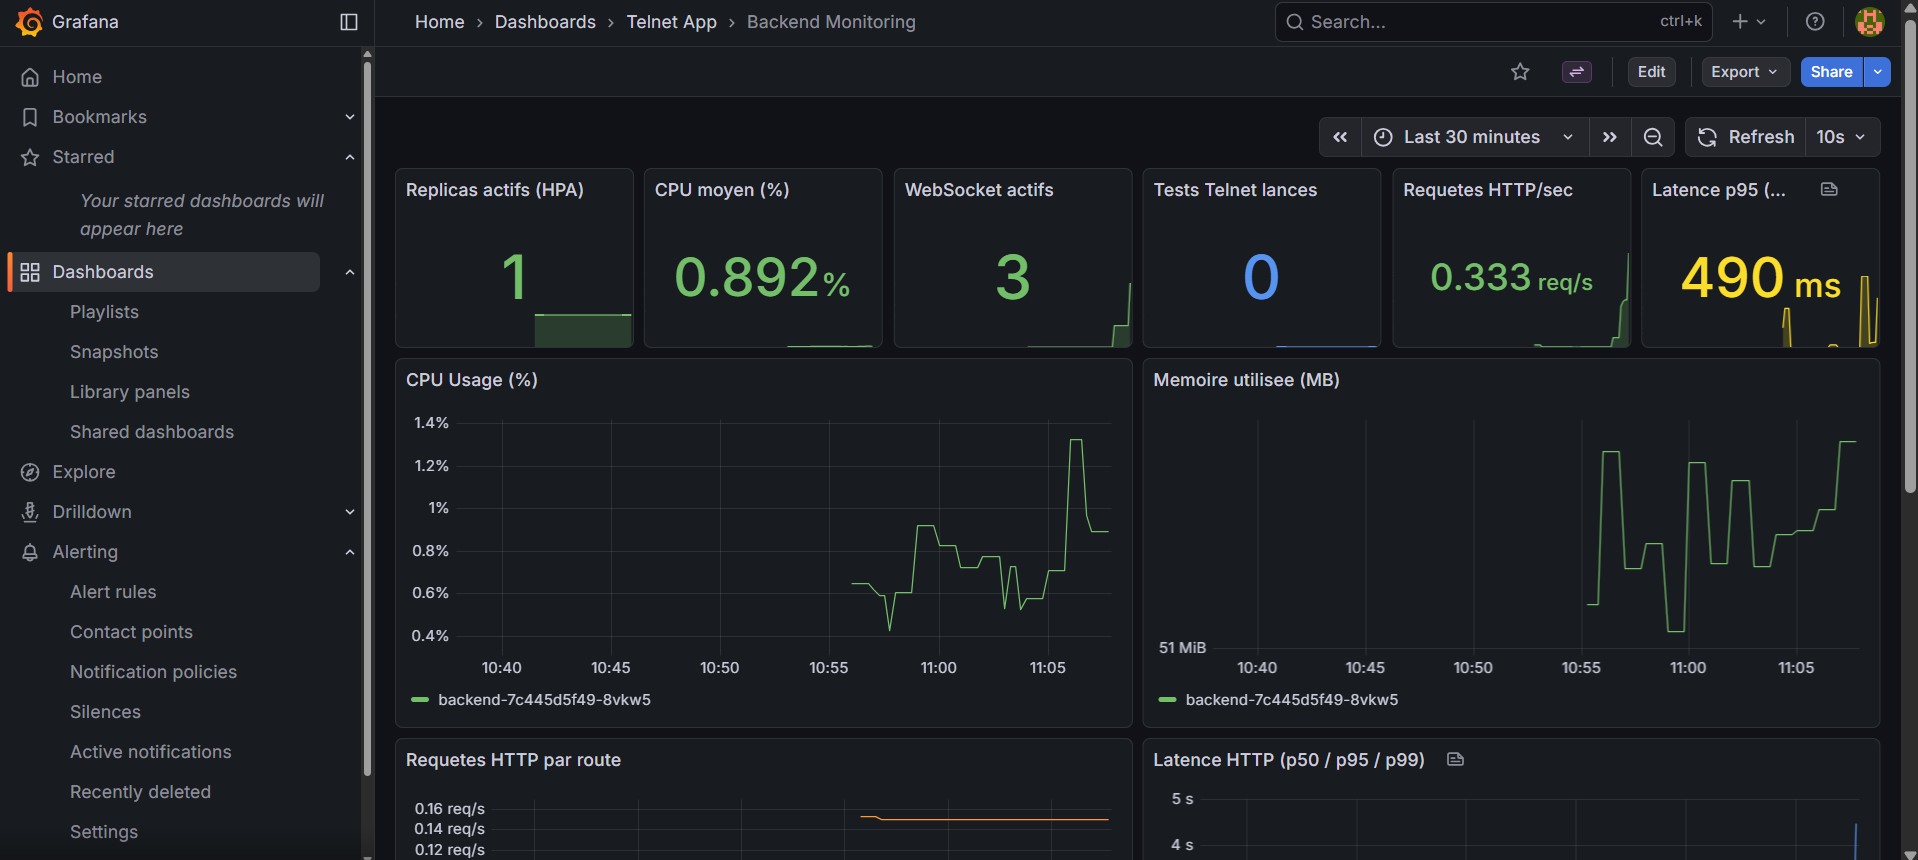
\includegraphics[width=\textwidth]{images/capture grafana metrics}
  \caption{Tableau de bord Grafana --- Telnet Test Manager}
  \label{fig:screen_grafana}
\end{figure}

\begin{figure}[H]
  \centering
  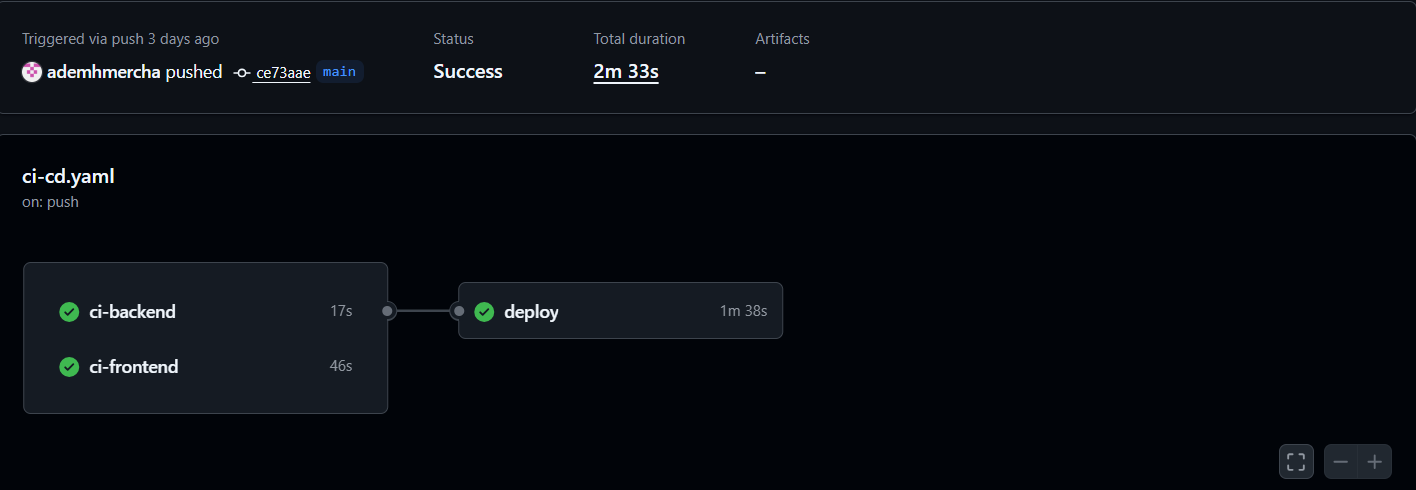
\includegraphics[width=\textwidth]{images/captre du pipeline}
  \caption{Capture d'écran~: exécution du pipeline CI/CD sur GitHub Actions}
  \label{fig:screen_pipeline}
\end{figure}

% -----------------------------------------------------------------
\section{Tests et validation}
% -----------------------------------------------------------------

\subsection{Stratégie de tests}

La qualité du projet est validée selon la \textbf{pyramide de tests}
classique~: un grand nombre de tests unitaires rapides, des tests
d'intégration couvrant l'API REST, et des tests fonctionnels manuels.

\begin{figure}[H]
  \centering
  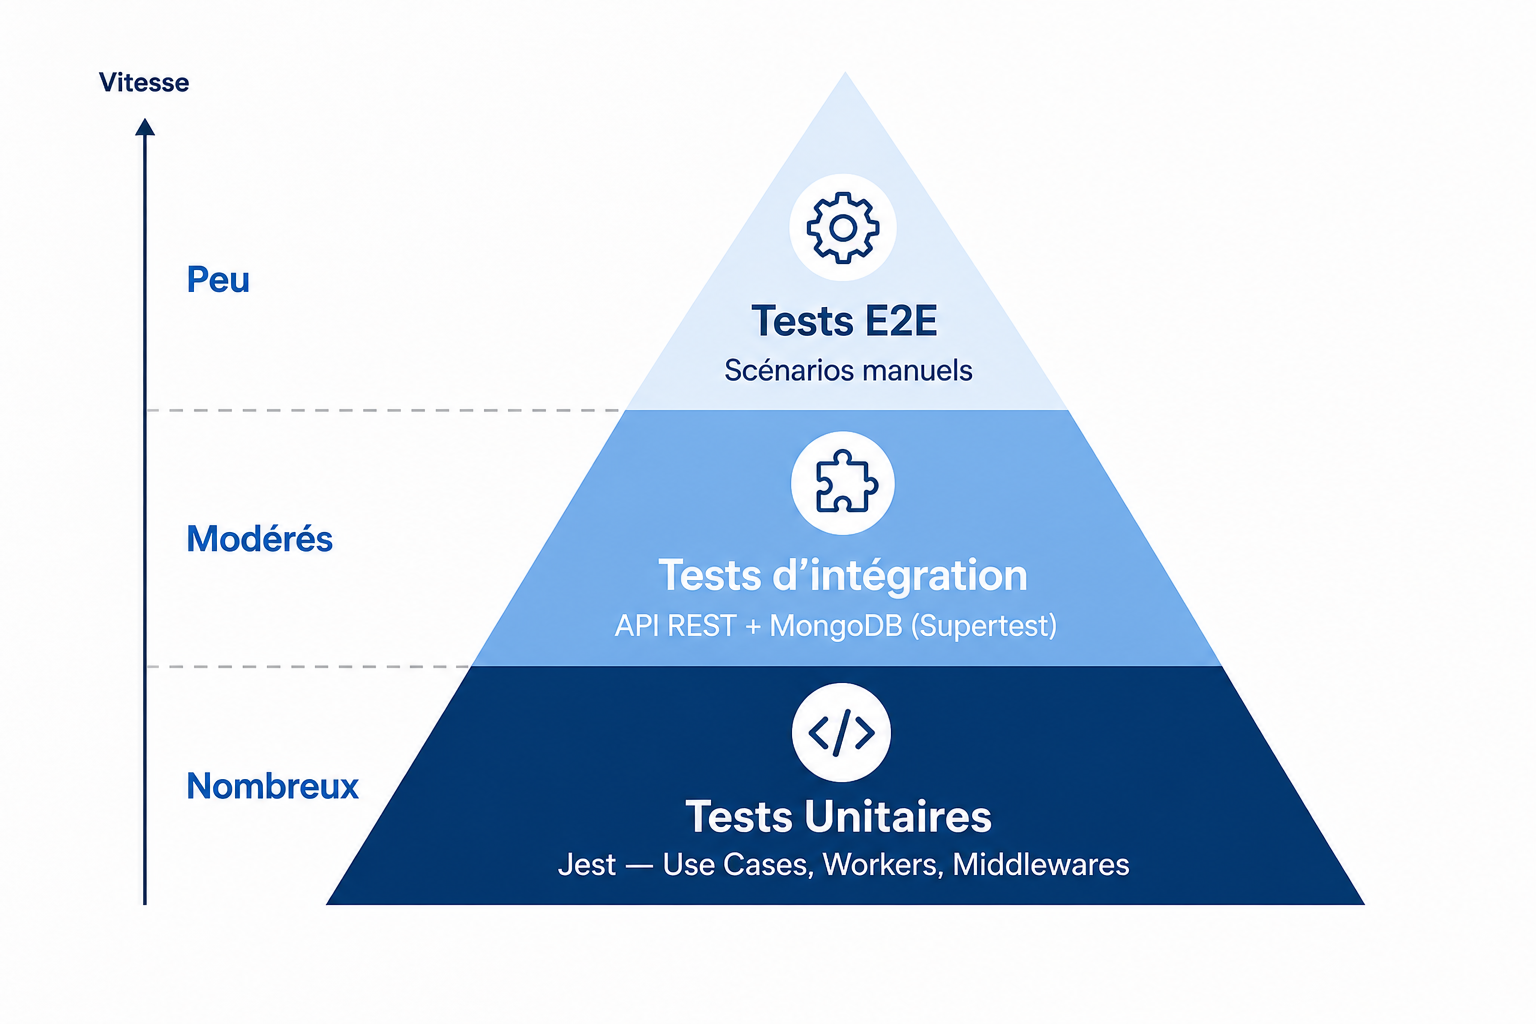
\includegraphics[width=0.75\textwidth]{images/pyramide_tests}
  \caption{Pyramide de tests adoptée pour Telnet Test Manager}
  \label{fig:test_pyramid}
\end{figure}

\subsection{Tests unitaires (Jest)}

Les tests unitaires couvrent les Use Cases et les modules critiques.
Les dépendances externes (MongoDB, réseau Telnet) sont mockées.

Deux cas de test couvrent le Use Case d'authentification~: le premier vérifie qu'un
appel avec des identifiants corrects retourne bien un objet contenant un champ
\texttt{token} (JWT signé)~; le second vérifie que l'exécution est rejetée avec
l'erreur \texttt{Compte inactif} lorsque le champ \texttt{statut} de l'utilisateur
vaut \texttt{inactif}. Le dépôt MongoDB est entièrement mocké via \texttt{jest.fn()},
garantissant l'isolation du test vis-à-vis de la base de données.

Les tests d'intégration utilisent \textbf{Supertest} avec une base
MongoDB de test isolée. Ils couvrent l'authentification, les endpoints
CRUD et la limitation de débit (rate limiting).

\begin{figure}[H]
  \centering
  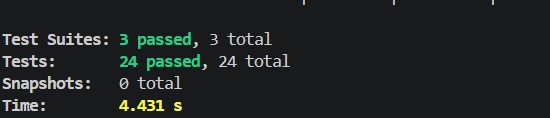
\includegraphics[width=0.7\textwidth]{images/jest_results}
  \caption{Résultats des tests Jest --- 24 tests passés sur 24 (3 suites)}
  \label{fig:screen_jest}
\end{figure}

\subsection{Tests fonctionnels (scénarios E2E)}

\begin{table}[H]
  \centering
  \caption{Scénarios de tests fonctionnels --- résultats}
  \label{tab:e2e_tests}
  \begin{tabularx}{\textwidth}{|C{1.2cm}|X|L{3.8cm}|L{2.2cm}|}
    \hline
    \textbf{ID} & \textbf{Scénario} & \textbf{Précondition} & \textbf{Résultat} \\
    \hline
    ST01 & Connexion identifiants valides   & Utilisateur actif en BD   & \textcolor{vertCode}{\textbf{PASS}} \\
    \hline
    ST02 & Connexion mot de passe erroné    & ---                       & \textcolor{vertCode}{\textbf{PASS}} \\
    \hline
    ST03 & Accès route protégée sans JWT    & ---                       & \textcolor{vertCode}{\textbf{PASS}} \\
    \hline
    ST04 & Création d'un Poste (CRUD)       & Rôle ingénieur            & \textcolor{vertCode}{\textbf{PASS}} \\
    \hline
    ST05 & Création Slot avec adresse IP    & Poste + Produit existants & \textcolor{vertCode}{\textbf{PASS}} \\
    \hline
    ST06 & Exécution test \texttt{single}   & Slot actif                & \textcolor{vertCode}{\textbf{PASS}} \\
    \hline
    ST07 & Exécution test séquence 3 étapes & Slot actif                & \textcolor{vertCode}{\textbf{PASS}} \\
    \hline
    ST08 & Résultats temps réel (WebSocket) & Test en cours             & \textcolor{vertCode}{\textbf{PASS}} \\
    \hline
    ST09 & Arrêt d'un test en cours         & Test PENDING              & \textcolor{vertCode}{\textbf{PASS}} \\
    \hline
    ST10 & Tests multi-slots (3 parallèles) & 3 slots configurés        & \textcolor{vertCode}{\textbf{PASS}} \\
    \hline
    ST11 & Génération d'un rapport          & Tests historisés           & \textcolor{vertCode}{\textbf{PASS}} \\
    \hline
    ST12 & Consultation journal d'audit     & Rôle admin                & \textcolor{vertCode}{\textbf{PASS}} \\
    \hline
    ST13 & Changement de langue (FR~$\to$~EN) & ---                     & \textcolor{vertCode}{\textbf{PASS}} \\
    \hline
    ST14 & Accès technicien à route admin   & JWT technicien            & \textcolor{vertCode}{\textbf{PASS}} \\
    \hline
  \end{tabularx}
\end{table}

\subsection{Résultats du pipeline CI/CD}

\begin{table}[H]
  \centering
  \caption{Résultats du pipeline GitHub Actions}
  \label{tab:cicd_results}
  \begin{tabularx}{\textwidth}{|L{2.5cm}|X|L{2.8cm}|L{2.5cm}|}
    \hline
    \textbf{Job} & \textbf{Étapes clés} & \textbf{Durée} & \textbf{Statut} \\
    \hline
    ci-backend  & npm ci + audit + tests        & 17\,s         & \textcolor{vertCode}{\textbf{Success}} \\
    \hline
    ci-frontend & npm ci + audit + build        & 46\,s         & \textcolor{vertCode}{\textbf{Success}} \\
    \hline
    deploy      & Build Docker + Helm + rollout & 1\,min\,38\,s & \textcolor{vertCode}{\textbf{Success}} \\
    \hline
    \textbf{Total} & --- & \textbf{2\,min\,33\,s} & \textcolor{vertCode}{\textbf{Success}} \\
    \hline
  \end{tabularx}
\end{table}

\subsection{Tableau de synthèse de validation}

\begin{table}[H]
  \centering
  \caption{Synthèse de la validation par rapport aux besoins}
  \label{tab:synthese_validation}
  \begin{tabularx}{\textwidth}{|C{1.2cm}|X|L{3.8cm}|L{2.2cm}|}
    \hline
    \textbf{BF} & \textbf{Besoin} & \textbf{Méthode de test} & \textbf{Statut} \\
    \hline
    BF-01 & Authentification JWT           & Tests unit. + intégration  & \textcolor{vertCode}{Validé} \\
    \hline
    BF-02 & Gestion des équipements CRUD   & Tests intégration          & \textcolor{vertCode}{Validé} \\
    \hline
    BF-03 & Bibliothèque de commandes      & Tests intégration          & \textcolor{vertCode}{Validé} \\
    \hline
    BF-04 & Tests multi-slots parallèles   & Tests fonctionnels         & \textcolor{vertCode}{Validé} \\
    \hline
    BF-05 & Résultats temps réel (WS)      & Tests fonctionnels         & \textcolor{vertCode}{Validé} \\
    \hline
    BF-06 & Exécution test Telnet          & Tests unit. + fonctionnels & \textcolor{vertCode}{Validé} \\
    \hline
    BF-07 & Génération de rapports         & Tests fonctionnels         & \textcolor{vertCode}{Validé} \\
    \hline
    BF-08 & Administration (RBAC)          & Tests unit. + intégration  & \textcolor{vertCode}{Validé} \\
    \hline
    ---   & Pipeline CI/CD                 & Exécution GitHub Actions   & \textcolor{vertCode}{Validé} \\
    \hline
    ---   & Déploiement Kubernetes         & \texttt{kubectl rollout}   & \textcolor{vertCode}{Validé} \\
    \hline
    ---   & Supervision Prometheus/Grafana & Consultation dashboard     & \textcolor{vertCode}{Validé} \\
    \hline
  \end{tabularx}
\end{table}

\section*{Conclusion}

Ce chapitre a détaillé l'infrastructure DevOps complète et la validation
du projet Telnet Test Manager. La conteneurisation Docker, l'orchestration
Kubernetes/Helm avec autoscaling HPA, le pipeline GitHub Actions en trois
jobs et la supervision Prometheus/Grafana constituent un système de
déploiement mature et automatisé. Le taux de réussite de 100\,\% sur les
14~scénarios fonctionnels testés et la validation de l'ensemble des
besoins fonctionnels confirment la qualité de la réalisation.

% =============================================================
%  Conclusion générale et perspectives
% =============================================================
\chapter*{Conclusion générale et perspectives}
\addcontentsline{toc}{chapter}{Conclusion générale et perspectives}
\markboth{Conclusion générale et perspectives}
         {Conclusion générale et perspectives}

Ce projet de fin d'études, réalisé au sein de \textbf{Sagemcom Ezzahra},
a abouti à la conception, au développement et au déploiement d'une
solution complète de tests Telnet automatisés pour les équipements réseau
embarqués. On est parti d'un processus manuel lent et fragmenté pour
livrer une plateforme web fullstack, intégrée dans une infrastructure
DevOps fonctionnelle et déployée automatiquement.

Sur le \textbf{plan applicatif}, \textbf{Telnet Test Manager} change
concrètement la façon dont les firmwares sont validés. L'application
est structurée selon les principes de la \textit{Clean Architecture}
en couches découplées (Domain, Application, Infrastructure, Interfaces),
ce qui facilite la maintenance et les évolutions futures. Le moteur
Telnet, basé sur les \textbf{Worker Threads} de Node.js, prend en
charge quatre modes~: commande unitaire, séquence pas-à-pas, supervision
continue et tests multi-slots en parallèle. Les résultats sont diffusés
en temps réel via \textbf{WebSocket} et l'interface \textbf{React~18/TypeScript}
est disponible en trois langues. Le contrôle d'accès \gls{rbac} à trois
rôles --- Administrateur, Ingénieur et Technicien --- gère les permissions
de façon claire et sécurisée.

Sur le \textbf{plan DevOps}, l'application est conteneurisée avec
\textbf{Docker} (build multi-stage qui ramène l'image frontend de
$\sim$900~Mo à $\sim$25~Mo en production) et orchestrée par un chart
\textbf{Helm} v0.3.0 sur \textbf{Kubernetes}. L'autoscaling horizontal
a été validé en conditions réelles~: lors des tests de charge, le CPU
a atteint 267\,\% du seuil, déclenchant automatiquement la montée de
1 à 5 répliques. Le \textbf{pipeline GitHub Actions} en trois jobs
gère l'intégration continue, les audits de sécurité et le déploiement
en 2~minutes~33~secondes via un runner auto-hébergé. \textbf{Prometheus}
et \textbf{Grafana} supervisent les métriques en temps réel et envoient
des alertes e-mail automatiques sur dépassement du seuil CPU.

Sur le \textbf{plan des tests}, les résultats sont clairs~: 24~tests
unitaires Jest passés à 100\,\%, 14~scénarios fonctionnels couvrant
tous les besoins identifiés, sans aucun échec sur l'ensemble de la
batterie de tests.

Pour l'équipe d'ingénierie des tests de \textbf{Sagemcom Ezzahra},
les bénéfices sont directs. Remplacer les terminaux manuels par une
interface web centralisée réduit le temps des campagnes de validation
et supprime les erreurs de saisie. Le journal d'audit et les rapports
automatiques permettent de suivre chaque campagne précisément.
L'architecture scalable et le déploiement automatisé donnent à l'équipe
une base solide pour faire évoluer la plateforme.

\section*{Perspectives d'évolution}

Les fondations établies par ce projet ouvrent plusieurs axes
d'amélioration pour les versions futures~:

\begin{itemize}
  \item \textbf{Support du protocole SSH~:} étendre le moteur de
        connexion pour couvrir les équipements modernes refusant
        les connexions Telnet non chiffrées~;

  \item \textbf{Analyse intelligente des résultats~:} appliquer
        des algorithmes de détection d'anomalies sur l'historique
        des tests pour anticiper les défaillances matérielles avant
        qu'elles n'affectent la production~;

  \item \textbf{Tests end-to-end automatisés~:} intégrer Cypress
        ou Playwright dans le pipeline CI/CD pour valider
        automatiquement les scénarios utilisateur complets~;

  \item \textbf{Déploiement cloud hybride~:} migrer vers AWS EKS
        ou GCP GKE pour étendre la portée de l'infrastructure à
        plusieurs sites géographiques de Sagemcom~;

  \item \textbf{Planification des campagnes~:} implémenter un
        module de scheduling pour lancer des campagnes de tests
        automatiques sur des plages horaires programmées.
\end{itemize}

\vspace{0.5cm}
\noindent Ce projet montre qu'en combinant une architecture logicielle
solide (\textit{Clean Architecture}, WebSocket, \gls{rbac}) avec des
pratiques \gls{devops} concrètes (Docker, Kubernetes, CI/CD,
Prometheus/Grafana), il est possible de remplacer un processus manuel
fragmenté par une plateforme automatisée, traçable et scalable. Le
résultat est une infrastructure de tests qui s'adapte à la charge, se
déploie seule et laisse une trace de chaque action --- exactement ce
dont l'équipe de Sagemcom Ezzahra avait besoin.


%%% ── Bibliographie ──────────────────────────────────────────
\clearpage
\bibliographystyle{apalike}
\bibliography{references}
\addcontentsline{toc}{chapter}{Bibliographie}

\end{document}
